\documentclass[10pt]{book}
\usepackage[T1]{fontenc}

\usepackage{preamble}
\addbibresource{MP.bib}

\title{From Measure to Probability}
\subtitle{A probabilist's survey of measure-theoretic results}
\author{Feng Cheng\thanks{Email: \href{mailto:fecheng@uw.edu}{\texttt{fecheng@math.washington.edu}}. Affiliation: Department of Mathematics, University of Washington, Seattle, WA 98195, USA.}}
\date{Draft as of \today}

% \includeonly{chapters/1-measure-spaces}

% \makenomenclature
% \renewcommand{\nomname}{List of Symbols}

\begin{document}
\maketitle

\cleardoublepage
\pdfbookmark{Contents}{table-of-contents}
\tableofcontents

% \printnomenclature

\phantomsection
\chapter*{\Large Prologue}
\addcontentsline{toc}{part}{Prologue}
\chaptermark{Prologue}

This is the most ambitious writing project undertaken by the author so far as a math student, and he hopes he can finish it in two years. The author, as a probability student, did not excel in his real analysis courses (MATH 202AB at UC Berkeley) during his senior year. To compensate, the author aims to write an extensive and detailed note that surveys through all the major measure theory results of interest to a rigorous-minded mathematical probabilist.

Part I of this note will be devoted to measure theory in a general setting, while Part II will discuss results in probability spaces built on top of Part I. The author hopes that his commentary and the overall structure of the survey can help the readers (and himself) truly understand both abstract measure theory and probability theory from a measure-theoretic point of view.

This entire survey will be based on multiple sources, listed in the bibliography page. As the old saying goes, ``if you copy from one book that is plagiarism, but if you copy from ten books that is scholarship.''
\vspace{1\baselineskip}

\noindent Shanghai, August 2024 \hfill F.C.

\vspace{3\baselineskip}
The prerequisite for this survey notes is a strong background in undergraduate real analysis and familiarity with elementary probability theory. Some key results about normed spaces, Hilbert spaces, and topology will be assumed, and these can usually be found on any first-year graduate analysis texts. Some rudimentary familiarity with weak topology on Banach spaces will contribute to the understanding of weak and vague convergence of measures. We have also included appendices at the end of the survey, which discuss some of these facts at a high level.

\emph{Remarks on Notation.} In Part I we use $X$ to denote a nonempty set, but in Part II we use $X$ instead to denote a random variable. As a replacement a nonempty set is denoted by $S$. Oftentimes $S$ is a metric space with metric $\rho$.
 
If you see any errors or typos, please inform the author via \begin{center}
    \href{mailto:fecheng@uw.edu}{\texttt{fecheng@math.washington.edu}}.
\end{center}

\part{Measure theory}
\chapter{Measure spaces}
\section{Basic setup}
We let $X$ be a nonempty set in Part I.
\begin{defn}
    For $\{A_n\}_{n=1}^\infty\subseteq \wp(X)$, we define \[
        \limsup_{n \to \infty} A_n = \bigcap_{n=1}^\infty \bigcup_{m=n}^\infty A_m \quad \text{and}\quad \liminf_{n \to \infty} A_n = \bigcup_{n = 1}^\infty \bigcap_{m = n}^\infty A_m.
    \]
\end{defn}
Note $\bigcap$ can be seen as ``for all'' and $\bigcup$ can be seen as ``there exists''. Therefore $\limsup_n A_n$ consists of elements that belong to infinitely many $A_n$'s (spread out across $n \in \N$), while $\liminf_n A_n$ consists of elements that belong to all but finitely $A_n$ (the $n$'s at the beginning). To compare this with the $\limsup$ and $\liminf$ of a sequence of numbers, one may try the following exercise.

\begin{xca}
    Show that \begin{align*}
        \limsup_{n \to \infty}  A_n = A & \iff \limsup_{n \to \infty} \ind_{A_n} = \ind_A, \\
        \liminf_{n \to \infty}  A_n = A & \iff \liminf_{n \to \infty} \ind_{A_n} = \ind_A.
    \end{align*}

    Here $\ind_A\colon X \to \{0,1\}$ given by \[
        \ind_A(x)= \begin{cases}
            1 & \text{if } x \in A, \\
            0 & \text{if } x \not\in A.
        \end{cases}
    \]
    is called the \df{indicator function} (\df[characteristic function (measure theory)]{characteristic function} for analysts who choose to write $\chi_A$).
\end{xca}

If $\{A_n\}_{n=1}^\infty$ is an increasing sequence of sets, then \[
    \liminf_n A_n = \limsup_n A_n = \bigcup_n A_n;
\] if the sequence is decreasing, then \[
    \liminf_n A_n = \limsup_n A_n = \bigcap_n A_n.
\] Also remember that, by De Morgan's Law, \[
    \limsup_n A_n^\cpl = \bigl(\liminf_n A_n\bigr)^\cpl \quad \text{and}\quad 
    \liminf_n A_n^\cpl = \bigl(\limsup_n A_n \bigr)^\cpl.
\]

Here is another exercise.

\begin{xca}
    Consider a sequence of functions $f_n$ that convergences to $f$ pointwise on some set $E$. If we define \[
        E_{n,\epsilon} = \{x:\abs{f_n(x) - f(x)} < \epsilon\}
    \] for $\epsilon > 0$ and $n\in \N$, then \[
        E = \bigcap_{k=1}^\infty \liminf_m E_m^{1/k} = \bigcap_{k=1}^\infty \bigcup_{m=1}^\infty \bigcap_{n\geq m} E_n^{1/k}.
    \]
\end{xca}

\begin{defn}
    A nonempty collection of subsets of $X$ is an \df{algebra} if \begin{enumerate}
        \item $\emptyset,X \in \A$;
        \item closed under complement;
        \item \label{enu:algebra-finite-union} closed under finite unions and intersections.
    \end{enumerate}
    Furthermore, $\A$ is called a \df[sigma-algebra@$\sigma$-algebra]{$\sigma$-algebra} if condition~\ref{enu:algebra-finite-union} asks for countable unions and intersections.
\end{defn}

An algebra can be constructed from a more basic structure called semialgebra, which we define below.
\begin{defn}
    A \df{semialgebra} $\mathcal{E}$ is a collection of sets such that \begin{enumerate}
        \item \label{enu:cond1-semialgebra}$\emptyset \in \mathcal{E}$;
        \item closed under finite intersections;
        \item if $A \in \mathcal{E}$ then $A^\cpl$ is a finite disjoint union of elements in $\mathcal{E}$.
    \end{enumerate}
\end{defn}
Some authors drop condition~\ref{enu:cond1-semialgebra}, while others add the condition that $X \in \mathcal{E}$. But of course there is no essential difference. Now comes the main result.

\begin{prop}[{\cite[Proposition~1.7]{folland1999}}] \label{prop:semialgebra-to-algebra}
    If $\mathcal{E}$ is a semialgebra\footnote{Folland calls this elementary family.}, then all finite disjoint unions of sets in $\mathcal{E}$ form an algebra.
\end{prop}

The most important example of a semialgebra consists of the empty set and all sets of the form \[
    (a_1,b_1] \times \dotsb \times (a_d,b_d] \subseteq \R^d,
\] where $-\infty \leq a_j<b_j \leq \infty$. The finite disjoint unions of half-open half-closed cubes should therefore form an algebra.

From now on we will assume $\A$ is by default a $\sigma$-algebra. Obviously the largest $\sigma$-algebra on $X$ is the power set $\wp(X)$.

Given a $\sigma$-algebra $\A$ on $X$, the couplet $(X,\mathcal{A})$ is called a \df{measurable space}, a space on which we can possibly attach a measure. Given a measurable space $(X,\A)$, we call a set $E$ is $\A$-measurable if $E\in \A$.

Also in analysis, ``$\sigma$'' means countable union while ``$\delta$'' means countable intersection. An \df[F-sigma set@$F_\sigma$ set]{$F_{\sigma}$ set} is a countable union\footnote{\emph{somme} in French} of closed\footnote{\emph{fermé} in French} sets, while a \df[G-delta set@$G_\delta$ set]{$G_\delta$ set} is a countable intersection\footnote{\emph{Durchschnitt} in German} of open\footnote{\emph{Gebiet} in German} sets.

We know that the preimage of a function $f\colon X \to Y$ is a mapping $f^{-1}\colon \wp(Y) \to \wp(X)$ that preserves unions, intersections, and complements, which are also operations in the definition of a $\sigma$-algebra. The next result makes the relationship between the two explicit. See \cref{sec:measurable-functions} for the use.
\begin{prop}[{\cite[Lemma 1.3]{Kallenberg_2002}}] \label{prop:induce-s-alg-meas-map}
    Consider $f\colon X \to Y$, and $\mathcal{M}$ and $\mathcal{N}$ be two respective $\sigma$-algebras on $X$ and $Y$. The preimage $f^{-1}$ induces two $\sigma$-algebras: \begin{enumerate}
        \item \label{enu:backward-ind-s-alg} $\mathcal{M}' =\{f^{-1}(A) : A \in \mathcal{N}\}$ on $X$, in the backward direction; 
        \item \label{enu:forward-ind-s-alg} $\mathcal{N}' = \{B \subseteq Y : f^{-1}(B) \in \mathcal{M}\}$ on $Y$, in the forward direction.
    \end{enumerate}
\end{prop}

\begin{defn}
    Within $X$, given a family of subsets $\mathcal{S}$, the smallest $\sigma$-algebra containing $\mathcal{S}$, i.e., the intersection of all $\sigma$-algebras that contains $\mathcal{S}$, is called the \df[sigma-algebra generated by@$\sigma$-algebra generated by!sets]{$\sigma$-algebra generated by $\mathcal{S}$} , denoted by $\sigma(\mathcal{S})$.

    Similar definitions hold for other types of structures.
\end{defn}
Remember the phrase ``the generated is the smallest'', and this should indicate how some proofs should proceed.

Check that the intersection of a family of algebras/$\sigma$-algebras is an algebra/$\sigma$-algebra. Note that the union is not.

If $X$ is a topological space, then the \df[Borel sigma-algebra@Borel $\sigma$-algebra]{Borel $\sigma$-algebra} on $X$, which we denote by $\B_X$ or $\B(X)$, is the $\sigma$-algebra generated by all open sets. One can of course replace the ``open'' here by ``close''.

If $X = \R$ with the standard Euclidean topology, then $\B(\R)$ is generated  
\begin{itemize}
    \item by open intervals (or closed), 
    \item by left-open right-closed intervals (or the other way around), 
    \item by open rays $\{(a,\infty):a\in\R\}$ (or the other way around),
    \item or by close rays $\{[a,\infty):a\in\R\}$ (or the other way around).
    \item One may replace the endpoints of intervals by rationals as well.
\end{itemize}

The first bullet point boils down the fact that an open set in $\R$ can always be written into the disjoint union of a countable number of open intervals. The proof of this requires us to show that 

\begin{xca}
    Given a set $U$ open in $\R$. The relationship $\sim$ on $U$ given by $x \sim y$ if $[x \land y, x \lor y] \subseteq U$ is an equivalence relation.
\end{xca}
The theorem is of significant importance throughout measure theory, and is key to the construction of Lebesgue measure on the real line that we will see soon. The notations $x \land y$ and $x \lor y$ are shorthand for $\min\{x,y\}$ and $\max\{x,y\}$. We will use them later more often.

\begin{defn}
     A \df{measure} $\mu$ on $(X,\A)$ is a function $\mu\colon\A\to[0,\infty]$ such that \begin{enumerate}
         \item $\mu(\emptyset) = 0$;
         \item \label{enu:countable-additivity-positive-measure} $\mu$ is \df[countably additive/$\sigma$-additive], i.e., let $\{E_n\}_{n=1}^\infty$ be any measurable partition of $E \in \A$, we have  \[
            \mu(E) = \mu\biggl(\bigcup_{n=1}^\infty E_n\biggr) = \sum_{n=1}^\infty \mu(E_n).
         \]
     \end{enumerate}
\end{defn}

For two different rearrangements of the same measurable partition of $E$, $\mu(E)$ should have the same value, because the sum of nonnegative values does not change under reordering. An easy way to see this is to note \[
    \sum_{n=1}^\infty a_n= \sup\biggl\{\sum_{n\in I} a_n:I\text{ is a finite subset of }\N\biggr\}.
\] In fact the RHS above is how we define generalized sums over possibly uncountable indices. Therefore condition~\ref{enu:countable-additivity-positive-measure} makes sense.

From now on we assume by default that $\mu$ is a measure. The triplet $(X,\A,\mu)$ is called a \df{measure space}.

A measure $\mu$ on $(X,\A)$ is a \df{probability measure}\footnote{Why use this name? Because the probability of the entire sample space should be 1.} if $\mu(X) = 1$; $\mu$ is \df[finite measure]{finite} if $\mu(X) < \infty$; and $\mu$ is \df[sigma-finite measure@$\sigma$-finite measure]{$\sigma$-finite} if $X$ can be written as a countable union of measurable sets $A_n \in \A$, each of which is of finite measure. Note for a $\sigma$-finite measure, we can replace this countable collection of finite-measure sets that make up $X$ by an increasing sequence of finite-measure sets. We may even further assume that the sets are mutually disjoint. These assumption can be handy in some proofs.

It is clear that any probability measure is a finite measure, which is in turn a $\sigma$-finite measure. The probability measure is the essential example of a finite measure, because mostly you can normalize the measure of the whole space to $1$.

A $\sigma$-finite measure is a well-behaved kind of measure. The Lebesgue measure that we will rigorously see soon, for example, is $\sigma$-finite. Some major results in measure theory, for example the Fubini--Tonelli theorem (see \cref{sec:prod-integrate}), are only true for $\sigma$-finite measure spaces. A measure that is not $\sigma$-finite is considered, in some sense, a little pathological.

The following facts will come up a couple of times.
\begin{fact} \label{fact:restrict-meausre-original-space}
    Fix some $S \in \A$. The function $\nu\colon \A\to [0,\infty]$ given by $\nu(E) = \mu(E \cap S)$ is still a measure on $(X,\A)$.
\end{fact}
\begin{fact} \label{fact:restrict-meausre-restrict-space}
    Fix $S\in \A$. By intersecting $S$ we can get a sub-$\sigma$-algebra $\A|_S$ on $S$, where \[
        \A|_S = \{E \cap S: E\in\A\}.
    \] Such $(S,\A|_S)$ is called a \df{measurable subspace} of $(X,\A)$. Note that $\mu$ restricted to the $\sigma$-algebra $\A|_S$ is a measure on $\A|_S$. We denoted this restricted measure on $(S,\A|_S)$ by $\mu|_S$, or simply $\mu$ when the context is clear. 
\end{fact}

Below are some important basic properties about measures that are used all the time.
\begin{prop}\label{prop:basic-properties-measure}
    We have the following properties about a measure $\mu$ on $(X,\A)$.
    \begin{enumerate}
        \item monotonicity: for $A,B\in \A$, \[
            A\subseteq B \implies \mu(A)\leq \mu(B);
        \]
        \item inclusion-exclusion: for $A,B \in \A$ with $\mu(A \cap B) < \infty$, we have \[
            \mu(A \cup B) = \mu(A) + \mu(B) - \mu(A\cap B).
        \]
        \item \df[sigma-subadditivity@$\sigma$-subadditivity]{$\sigma$-subadditivity}: for possibly intersecting sets\footnote{Recall in $\sigma$-additivity the sets must be mutually disjoint.} $\{E_n\}_{n=1}^\infty \subseteq \A$, \[
            \mu\biggl(\bigcup_{n=1}^\infty E_n\biggr) \leq \sum_{n=1}^\infty \mu(E_n).
        \]
        \item continuity from below: for a sequence of sets $\{E_n\}_{n=1}^\infty \subseteq \A$ that increases to $E$, we have \[
            \mu(E_n) \uparrow \mu(E).
        \]
        \item continuity from above (when the first set is of finite measure): for a sequence of sets $\{E_n\}_{n=1}^\infty \subseteq \A$ with $\mu(E_1)<\infty$ and $E_n \downarrow E$, we have \[
             \mu(E_n) \downarrow \mu(E).
        \]
    \end{enumerate}
\end{prop}
All these properties above require the famous disjointification trick to prove: we partition the sets in question into pairwise disjoint pieces, and then use countable additivity of the measure.

Now we discuss two important examples of measure extremely useful in application\footnote{In this note we will avoid going deep into facts/examples/counterexmaples that are ultimately not very useful in practice. One such ``useless'' example that is often mentioned here is the countable-cocountable measure on an uncountable set. One may also list the collection of all countable and cocountable sets as an example of a $\sigma$-algebra earlier, but we have omitted for the same reason. Some results of greater generality and particular examples add further insight to the subject matter and help our understanding, but in many situations this is not the case.}.

The first one is the \df{counting measure}. Consider the measurable space $\bigl(X,\wp(X)\bigr)$. The function $\mu\colon \wp(X) \to [0,\infty]$ given by $\mu(E) = \abs{E}$ is a measure. Basically it counts how many elements are in each subset of $X$.

The second one is the \df{Dirac point mass}. Given $(X,\A)$ and some $x\in X$, we define the function $\delta_X\colon \A \to \{0,1\}$ given by \[
    \delta_x(A) = \begin{cases}
        1 & \text{if } x \in A, \\
        0 & \text{if } x \not\in A.
    \end{cases}
\]
This is clearly a probability measure. Notice its difference from the indicator function. The point mass $\delta_x(A)$ takes in a set and spits out $1$/$0$, while the corresponding indicator $\ind_A(x)$ takes in a point and spits out $1$/$0$.

A countable linear combination of Dirac point mass defines a measure $\mu$ on $\A$ called the \df{discrete measure} To be precise, given a countable set $Y \subseteq X$, and a function $c\colon y \mapsto [0,\infty]$ at each $y \in Y$, we can define $\mu\colon \A \to \infty$ by \[
    \mu = \sum_{y \in Y} c(y)\delta_y.
\] The meticulous reader should notice that the function $c$ here resembles the probability mass function on a discrete probability space; see \cref{sec:dist}.

We now introduce two additional elementary results about measures, which are simple consequences from \cref{prop:basic-properties-measure}. These two results are important in probability theory, but both are indeed purely measure-theoretic.
\begin{cor}[(Upper and lower semicontinuity of measures)]
    For $\{E_n\}_n \subseteq \A$, we have \[
        \mu\bigl(\liminf_n E_n\bigr) \leq \liminf_n \mu(E_n).
    \]
    If in addition $\mu$ is finite, then \[
        \limsup_n \mu(E_n) \leq \mu\bigl(\limsup_n E_n\bigr).
    \]
\end{cor}

\begin{namedthm}[Borel--Cantelli lemma I] \label{thm:BorelCantelli-meas-th}
    For $\{E_n\}_n \subseteq \A$, assume $\sum_{n} \mu(E_n) <\infty$, then \[
        \mu\bigl(\limsup_n E_n\bigr) = 0.
    \]
\end{namedthm}

We will see that the above result will be used to prove almost everywhere convergence of functions, a notion that will be introduced in \cref{chap:meas-func-int}.

One can skip the rest of this section for now, and come back after reading about the Lebesgue measure on the real line.

Given $(X,\A,\mu)$, a subset $E\subseteq X$ is called a \df{null set}
if there is $B\in\mathcal{A}$ such that $E\subseteq B$ and $\mu(B)=0$.
If $\A$ contains all these null sets, then the measure space is \df{complete}.
The \df{completion} $\A^\mu$ is the smallest $\sigma$-algebra containing $\A$ such that there exists a measure $\bar{\mu}$, which extends $\mu$ to $\A^\mu$, that makes $(X,\A^\mu)$ complete.

Why is a complete measure space sometimes desirable? In some cases we want to make all subsets of measure zero sets measurable to avoid some technical peculiarity, and meanwhile we can measure a larger collection of sets. However, it is important to remember that a larger $\sigma$-algebra can lead to more technical peculiarities as well. In many cases the additional measurable sets after completion may not be well-behaved with respected functions, which we will see in \cref{sec:measurable-functions}. In addition, even a complete measure space $(X,\A,\mu)$ may still not measure every subset of $X$.

The completion of a measure space is given explicitly, as stated in the following theorem.

\begin{thm}[{\cite[Theorem 1.9]{folland1999}}]
    The completion $\A^\mu$ is unique, which is given by \[
        \A^\mu =\{E\cup F:E\in\A\text{ and }F\subseteq N\text{, where }N\text{ is a null set}\}.
    \]
    In addition, the measure $\bar{\mu}$ given by $\bar{\mu}(E\cup F)=\mu(E)$ not only completes $\A$, but also is the unique extension of $\mu$ from $\A$ to $\A^\mu$.
\end{thm}
\begin{proof}
    The first part of the proof is given in the reference. For the uniqueness part, suppose there is some other measure $\hat{\mu}$ on $\A^\mu$ such that $\hat{\mu}(E) = \mu(E)$ for all $E \in \A$. However, there exists some $D \subseteq N$, where $\mu(N) = 0$, such that $\hat{\mu}(E \cup D) \neq \mu(E) = \hat{\mu}(E)$. This implies $\hat{\mu}(D - E) > 0$. Yet $D - E \subseteq N$ where $\hat{\mu}(N) = 0$. This contradicts monotonicity.
\end{proof}

To similarly avoid peculiarities caused by null sets, we give the following definitions. Let $\mu$ be a finite measure. The set $A \in \A$ is called an \df{atom} of the measure $\mu$ if the set has measure $\mu(A) > 0$, but all its measurable subsets must be either of measure $0$ or of measure $\mu(A)$. A measure is \df[atomless measure]{atomless} if there are no atoms. A measure $\mu$ is \df[purely atomic measure@(purely) atomic measure]{(purely) atomic} if the measure $\mu$ is concentrated on a countable union of atoms $\cup_{n=1}^\infty A_n$, i.e., $\mu(X - \cup_n A_n) = 0$.

\section{Two tools from set theory}
\begin{defn}
A \df[pi-system@$\pi$-system]{$\pi$-system} on $X$ is a nonempty collection of subsets of $X$ that is closed under finite intersections.

A \df[lambda-system@$\lambda$-system]{$\lambda$-system} $\mathcal{L}$ on $X$ is a collection of subsets of $X$ such that 
\begin{enumerate}
    \item $X\in\mathcal{L}$; 
    \item \label{enu:prop-diff-lam-sys} if $A,B\in\mathcal{L}$ and $A\subseteq B$, then $B-A\in\mathcal{L}$; (closed under proper differences)
    \item if $A_{n}\in\mathcal{L}$ and $A_{n}\uparrow A$ then $A\in\mathcal{L}$. (closed under ascending countable unions)
\end{enumerate}
\end{defn}
\begin{defn}
    A \emph{monotone class} on $X$ is a collection of subsets of $X$ that is closed under ascending countable unions and descending countable intersections.
    
\end{defn}
\begin{namedthm}[Dynkin's $\pi$-$\lambda$ theorem] \label{thm:pi-lambda}
     Within $X$, if $\mathcal{K}$ is a $\pi$-system that is contained in a $\lambda$-system $\mathcal{L}$, then $\sigma(\mathcal{K})\subseteq\mathcal{L}$.
\end{namedthm}
\begin{namedthm}[Monotone class theorem] \label{thm:monotone-class}
     Given an algebra $\A_0$ of sets, then the monotone class $\mathcal{M}$ generated by $\A_0$ coincides with the $\sigma$-algebra $\sigma(\A_0)$ generated by $\A_0$.
\end{namedthm}

We do not prove these results in this note; they are very complicated and not very interesting in the end. ``The generated is the smallest'' is the main idea behind these proofs though. The proof of the next result should provide the readers with a general idea what proofs of this sort look like.

This next result is of theoretical significance. It tells us a $\pi$-system that generates the $\sigma$-algebra identifies the measure. 

Suppose we want to show some property holds on the entire $\A$. The way we apply the \nameref{thm:pi-lambda} usually looks like this. First we prove that the collection of sets with this property is a $\lambda$-system. If we have a $\pi$-system with this property that generates $\A$, then the entire $\A$ must agree with this $\lambda$-system.

\begin{namedthm}[Coincidence criterion {\cite[Proposition~1.15]{Ambrosio_2011}}]
    Let $\mu_1$ and $\mu_2$ be two measures on $(X,\A)$. Suppose we can find a $\pi$-system $\mathcal{K}$ on which the two measures agree, and $\sigma(\mathcal{K}) = \A$.

    If $\mu_1(X) = \mu_2(X) < \infty$ (for example, both are probability measures), then the two measures agree on the entire $\A$.

    More generally, if there exists $\{X_n\} \subseteq \mathcal{K}$ such that $X_n \uparrow X$ and \[
        \mu_1(X_n) = \mu_2(X_n) <\infty \text{ for all }n\in \N,
    \] then the two measures agree on the entire $\A$.
\end{namedthm}
\begin{proof}
    Assume $\mu_1(X) = \mu_2(X) < \infty$. Define $\mathcal{D}$ to be the collection of all sets in $\A$ on which the two measures agree. It is easy to verify that $\mathcal{D}$ becomes a $\lambda$-system. Now invoke \nameref{thm:pi-lambda} and conclude that $\mathcal{D} = \mathcal{A}$. Without the finiteness assumption, we cannot verify condition~\ref{enu:prop-diff-lam-sys} for a $\lambda$-system  that makes $\mu(B) - \mu(A)$ computable.

    Now consider the general assumption. We define for each $n$ \begin{align*}
        \A_n & = \{E \cap X_n : E \in \A\}\text{, which is a $\sigma$-algebra, and} \\
        \mathcal{K}_n & = \{E \cap X_n : E \in \mathcal{K}\}\text{, which is a $\pi$-system contained in $\A_n$.}
    \end{align*}
    Then $\mu_1$ and $\mu_2$ restricted to $(X_n,\A_n)$ is a finite measure. By the special case above, the two measures coincide on $\sigma(\mathcal{K}_n)$.

    Now we prove $\A_n \subseteq \sigma(\mathcal{K}_n)$. Check that since $X_n \in \mathcal{K}$, \[
        \{E \subseteq X : E \cap X_n \in \sigma(\mathcal{K}_n)\}
    \] is a $\sigma$-algebra containing $\mathcal{K}$, and hence $\A$.

    Now for each $n$ and all $E \in \mathcal{A}$, the two measures agree on $E \cap X_n$. Now take $n \to \infty$ and we see that $\mu_1 = \mu_2$.
\end{proof}

\section{Extension theorems}
\begin{defn}
    An \df{outer measure} on $X$ is a function $\mu^{*}\colon\wp(X)\to[0,\infty]$ such that 
    \begin{enumerate}
    \item $\mu^{*}(\emptyset)=0$; (emptyset)
    \item if $A\subseteq B$, then $\mu^{*}(A)\leq\mu^{*}(B)$; (monotonicity)
    \item For subsets $A_{1},A_{2},\dotsc$ of $X$, $\mu^{*}(\cup_{i=1}^{\infty}A_{i})\leq\sum_{i=1}^{\infty}\mu^{*}(A_{i})$. ($\sigma$-subadditivity)
    \end{enumerate}
    A \df[outer null set]{null set} with respect to the outer measure $\mu^{*}$ is just a set with $\mu^{*}$-value 0.
\end{defn}

Let $\mathcal{C}$ be a collection of subsets of $X$ such that $\emptyset\in\mathcal{C}$ and there are $D_{1},D_{2},\dotsc$ in $\mathcal{C}$ such that $\cup_{i\in\N}D_{i}=X$. Suppose $\ell\colon\mathcal{C}\to[0,\infty]$ with $\ell(\emptyset)=0$. Now if we define for all $E\in \wp(X)$ 
\[
    \mu^{*}(E)=\inf\biggl\{\sum_{i=1}^{\infty}\ell(A_{i}):E\subseteq\bigcup_{i=1}^{\infty}A_{i}\text{, where every }A_{i}\in\mathcal{C}\biggr\},
\]
then $\mu^{*}$ is an outer measure on $X$. (Note that by assumption
the infimum is taken over a nonempty set, and hence always exists. For simplicity one may just assume $X \in \mathcal{C}$ as well.)
The proof is routine.

    Here are some forewords to what we will construct.
\begin{itemize}
\item Let $X=\R$, $\mathcal{C}$ be the collection of all left-open right-closed
intervals, and $\ell\bigl((a,b]\bigr)=b-a$. This gives the Lebesgue
outer measure $m^{*}$ used to construct the Lebesgue measure $m$.
\item Let $f\colon\R\to\R$ be an increasing right-continuous\footnote{We will use ``increasing'' and ``strictly increasing'' in our note. Right-continuity at $x$ means continuity from $x^{+}$.}
function. we let $\ell\bigl((a,b]\bigr)=f(b)-f(a)$. The $\mu^{*}$
that arises from this is used to construct the Lebesgue--Stieltjes measure.
\end{itemize}

\begin{defn}
    For an outer measure $\mu^{*}$, a set $A\subseteq X$ is \df[outer measurable]{$\mu^{*}$-measurable} if for all $E\subseteq X$, \[
        \mu^{*}(E)=\mu^{*}(E\cap A)+\mu^{*}(E\cap A^\cpl).
    \] 
\end{defn}

    This characterizes a collection of sets that are well-behaved under set operations, which leads to the next theorem. Note it $A$ is $\mu^{*}$-measurable if and only if for all $E$ with $\mu^{*}(E)<\infty$, \[
        \mu^{*}(E)\geq\mu^{*}(E\cap A)+\mu^{*}(E\cap A^\cpl).\]
\begin{namedthm}[Carathéodory's theorem]
    Given an outer measure $\mu^{*}$ on $X$, then the collection $\A$ of $\mu^{*}$-measurable sets is in fact a $\sigma$-algebra on $X$. Let $\mu=\mu^{*}|_{\mathcal{A}}$, then $\mu$ is a measure. Also the $\sigma$-algebra $\A$ contains all the null sets, i.e., $(X,\A,\mu)$ is complete.
\end{namedthm}

\begin{proof}
$\A$ is clearly closed under complements. We then check $\A$ is an algebra (the union of two sets in $\A$ is still in $\A$), and show $\mu^{*}$ is finitely additive on $\A$.

We wish to extend finite additivity to countable additivity. We let
$B_{n}=\cup_{j=1}^{n}A_{j}$ and $B=\cup_{j=1}^{\infty}A_{j}$. For
any $E$, we may conclude that 
\[
\mu^{*}(E\cap B_{n})=\sum_{j=1}^{n}\mu(E\cap A_{j}).
\]
It follows that $\mu^{*}(E)\geq\sum_{j=1}^{n}\mu^{*}(E\cap A_{j})+\mu(E\cap B^{\mathrm{c}}).$
Take $n\to\infty$ we may conclude 
\begin{align*}
\mu^{*}(E) & \geq\sum_{j=1}^{\infty}\mu^{*}(E\cap A_{j})+\mu^{*}(E\cap B^{\mathrm{c}})\\
 & \geq\mu^{*}\Bigl(\bigcup_{j=1}^{\infty}(E\cap A_{j})\Bigr)+\mu^{*}(E\cap B^{\mathrm{c}})\\
 & =\mu^{*}(E\cap B)+\mu^{*}(E\cap B^{\mathrm{c}})\geq\mu^{*}(E).
\end{align*}
It follows that $B\in\A$, and if we let $E=B$, the first inequality
(which is an equality) gives countable additivity.

It is easy to show $\A$ contains all $\mu^{*}$-null sets: for $N$
such that $\mu^{*}(N)=0$, for any $E$ we have 
\[
\mu^{*}(E)\leq\mu^{*}(E\cap N)+\mu^{*}(E\cap N^{\mathrm{c}})\leq\mu^{*}(E\cap N^{\mathrm{c}})\leq\mu(E).\qedhere
\]
\end{proof}

\begin{namedthm}[Carathéodory extension theorem] \label{thm:Caratheodory-ext}
    For algebra $\A_{0}$ on $X$ and its premeasure
$\mu_{0}$, let 
\[
\mu^{*}(E)=\inf\biggl\{\sum_{i=1}^{\infty}\mu_{0}(A_{i}):E\subseteq\bigcup_{i=1}^{\infty}A_{i}\text{, where every }A_{i}\in\A_{0}\biggr\}
\]
for all $E\subseteq X$. Then (1) $\mu^{*}$ is an outer measure on $X$, and hence by Carathéodory's theorem it gives a meausure space
$(X,\sigma(\A_{0}),\mu)$; (2) $\mu^{*}|_{\A_{0}}=\mu_{0}$; (3) every
set in $\A_{0}$ is $\mu^{*}$-measurable; (4) if $\mu_{0}$ is $\sigma$-finite,
then $\mu$ in (1) is the unique extension of $\mu_{0}$ from $\A_{0}$
to $\sigma(\A_{0})$.
\end{namedthm}

\begin{proof}
When proving $\mu^{*}(E)\geq\mu_{0}(E)$ in (2), consider the disjoint
sets $B_{n}=E\cap(A_{n}-\cup_{i=1}^{n-1}A_{i})$. Then $\cup_{n=1}^{\infty}B_{n}=E$,
which implies $\sum_{n=1}^{\infty}\mu_{0}(A_{n})\geq\sum_{n=1}^{\infty}\mu_{0}(B_{n})=\mu_{0}(E)$.
Then take infimum. (3) is fairly straightforward from definition.

To prove (4), let measure $\nu$ be another extension. Consider $E\in\sigma(\A_{0})$
and $\{A_{i}\}_{i=1}^{\infty}\subseteq\A_{0}$ that covers $E$, we
have 
\[
\nu(E)\leq\sum_{i=1}^{\infty}\nu(A_{i})=\sum_{i=1}^{\infty}\mu_{0}(A_{i}).
\]
Take infimum and we get $\nu(E)\leq\mu(E)$.

Now let $A=\cup_{i=1}^{\infty}A_{i}$, then 
\[
\mu(A)=\lim_{n\to\infty}\mu(\cup_{i=1}^{n}A_{i})=\lim_{n\to\infty}\nu(\cup_{i=1}^{n}A_{i})=\nu(A).
\]
If $\mu(E)<\infty$, then for any $\epsilon>0$ we may choose $\{A_{i}\}_{i=1}^{\infty}$
such that $\mu(A-E)<\epsilon$. It follows that 
\[
\mu(E)\leq\mu(A)=\nu(A)=\nu(E)+\nu(A-E)<\nu(E)+\epsilon.
\]
 Therefore $\mu(E)=\nu(E)$.

Now suppose we have $X=\cup_{j=1}^{\infty}B_{j}$ such that $\mu_{0}(B_{j})<\infty$
and that the $B_{j}$'s are pairwise disjoint. Then for $E\in\sigma(\A_{0})$,
we have 
\[
\mu(E)=\sum_{j=1}^{\infty}\mu(E\cap B_{j})=\sum_{j=1}^{\infty}\nu(E\cap B_{j})=\nu(E),
\]
where the second equality follows from what we have previously.
\end{proof}

\section{The Lebesgue measure}
\begin{fact}
    Assuming the full axiom of choice, we can use Zorn's lemma to assert that $\mathcal{L} \neq \wp(X)$.
\end{fact}

\begin{fact}
    Assuming the countable axiom of choice, we can explicitly show that $\mathcal L \neq \mathcal B$.
\end{fact}

We know as a consequence of \cref{prop:semialgebra-to-algebra} that the finite disjoint unions of $(a,b]$, where $a,b\in \R$, form an algebra on $\R$. We refer to this algebra as $\A_0$ below.

\begin{thm} \label{thm:premeasure-h-intervals}
    For an increasing right-continuous function $F\colon \R \to \R$, the function $\mu_0\colon \A_0 \to [0,\infty]$ such that $\mu_0(\emptyset) = 0$ and \[
        \mu_0\biggl(\bigcup_{j=1}^n (a_j,b_j]\biggr) = \sum_{j=1}^n F(b_j) - F(a_j)\quad \text{for disjoint }\{(a_j,b_j]\}_{j=1}^n
    \] is countably additive, and hence a premeasure on $\A_0$.
\end{thm}

\begin{thm}[{\cite[Theorem~1.16]{folland1999}}] \label{thm:increasing-rcont-Borel-measure-connection} \leavevmode
    \begin{enumerate}
        \item \label{enu:CDF-measure} Let $F\colon \R \to \R$ be an increasing, right-continuous function, then there is a unique associated Borel measure $\mu_F$ on $\R$ such that \[
            \mu_F(a,b] = F(b) - F(a)\quad \text{for all }a\leq b.
        \]
    If $G$ is another increasing, right-continuous function, then $\mu_F = \mu_G$ if and only if $F$ and $G$ differ by a constant.
        \item \label{enu:measure-CDF} Conversely, if $\mu$ is a finite Borel measure on $\R$, then the function $F\colon \R \to \R$ given by $F(x) = \mu(-\infty,x]$ is increasing and right-continuous. Furthermore $\mu = \mu_F$, and the function has left limits, i.e., $\lim_{y \to x^-} F(y)$ exists at every $x \in \R$. More specifically, \begin{equation} \label{eq:CDF-left-limits}
             \lim_{y \to x^-} F(y) = \mu(-\infty,x).
        \end{equation}
    \end{enumerate}
\end{thm}

Regarding equation \eqref{eq:CDF-left-limits}, it is customary to write $F(x-) = \lim_{y \to x^-} F(y)$ when the limit exists. Note that having left limits implies \[\mu\{x\} = F(x) - F(x-)\] for all $x \in \R$.

\begin{proof} \leavevmode
    \begin{enumerate}
        \item Following \cref{thm:premeasure-h-intervals}, we have a premeasure $\mu_0$ on $\A_0$ given by \[
          \mu_0(a,b] = F(b) - F(a).
        \] Note $\mu_0$ is $\sigma$-finite as $\R = \cup_{j\in \Z} (j,j+1]$. Therefore by \nameref{thm:Caratheodory-ext}, it has a unique extension to a measure on $\sigma(\A_0) = \B(\R)$.
        
        The $\mu_F = \mu_G$ if and only if $F - G$ is a constant part is easy.
        \item $F$ is increasing because $\mu$ is a nonnegative function. Right-continuity follows from \begin{align*}
            \lim_{y \to x^+} F(y) & = \lim_{y \to x^+} \mu(-\infty,y] \\ & = \lim_{n\to \infty} \mu\Bigl(-\infty,x+\frac{1}{n}\Bigr]\\& = \mu\biggl(\bigcap_{n=1}^\infty \Bigl(-\infty,x+\frac{1}{n}\Bigr]\biggr) \\
            & = \mu(-\infty,x] = F(x).
        \end{align*} Note that the second equality is justified because $\lim_{y \to x^+} F(y)$ exists in the first place.

        To show $\mu = \mu_F$, we check for any $a \leq b$, \begin{align*}
            \mu(a,b] & = \mu(-\infty,b] - \mu(-\infty,a] \\
                & = F(b) - F(a),
        \end{align*} and use part~\ref{enu:CDF-measure}.

        It remains to show for every $x \in \R$ that \eqref{eq:CDF-left-limits} holds: \begin{align*}
            \lim_{y \to x^-} F(y) & = \lim_{y \to x^-} \mu(-\infty,y] \\ 
            & = \lim_{n \to \infty} \mu\Bigl(-\infty,x-\frac{1}{n}\Bigr] \\
            & = \mu\biggl(\bigcup_{n=1}^\infty\Bigl(-\infty, x -\frac{1}{n}\Bigr]\biggr) \\
            & = \mu(-\infty,x). \qedhere
        \end{align*}
    \end{enumerate}
\end{proof}

    For part~\ref{enu:measure-CDF}, if $\mu$ is a Borel measure on $\R$ that is finite on all bounded Borel sets, then $F$ can be instead defined by \[
        F(x) = \begin{cases*}
            \mu (0,x] & if $x > 0$, \\
            0 & if $x = 0$, \\
            -\mu(x,0] & if $x < 0$,
        \end{cases*}
    \] and all conclusions still hold.

    In the context of part~\ref{enu:CDF-measure}, the $\mu_F$ is called the \df{Lebesgue--Stieltjes measure} associated to $F$. When the function $F$ is the identity function, $\mu_F$ is called the \df{Lebesgue measure} on $\R$, which we will denote by $m$ in this note\footnote{Other common notations include $\lambda,\mathcal L,\abs{\blank}$.}. It generalizes the notion of length of intervals to a wide collection of subsets of $\R$, that is sufficient for application most of the time.
    
    In some cases it is useful to consider the completion of $(\R,\B,\mu_F)$, so that we can measure more sets than the Borel sets. The completion of $\B$ with respect to the Lebesgue measure $m$ is called the Lebesgue $\sigma$-algebra, which we denote by $\mathcal L$. 
    
\begin{thm}
    The Lebesgue measure $m$ on $(\R,\B)$ is the only nontrivial measure, up to multiplicative constants, that is translation invariant and locally finite.
\end{thm}

\section{Regularity of measures}
\begin{defn}
    A measure $\mu$ on $(X,\A)$ is \df{outer regular} if for all $E\in \A$, \[
        \mu(E) = \inf\{\mu(G): G\text{ is open in }X \text{ and } G\supseteq E\};
    \] it is \df{closed inner regular} if \[
        \mu(E) = \sup\{\mu(F): F\text{ is closed in }X \text{ and } F\subseteq E\};
    \] it is \df{compact inner regular} if \[
        \mu(E) = \sup\{\mu(K): K\text{ is compact in }X  \text{ and } K\subseteq E\}.\]
    We say a finite measure $\mu$ is \df[tight measure]{tight} if \[
        \mu(X) = \sup\{\mu(K): K\text{ is compact in }X  \text{ and } K\subseteq X\}.
    \]
\end{defn}

\begin{prop}
    Every finite measure on a topological space is outer regular if and only if it is closed inner regular.
\end{prop}

The proof is obvious. If a set is outer regular, then its complement is inner regular.

\begin{thm}[{\cite[Theorem~1.1]{Billingsley_1999}}]
    For a finite measure $\mu$ on a metric space $X$ with the Borel $\sigma$-algebra, $\mu$ is both outer regular and closed inner regular. It follows that a tight Borel measure is compact inner regular, by \cref{prop:closed-compact-intersect}.
\end{thm}
\begin{proof}
    Here is a common way to characterize the regularity of measures: for all $E\in \B(X)$, for all $\epsilon$, there exist closed $F$ and open $G$ such that $F\subseteq E \subseteq G$ with $\mu(G - F) < \epsilon$. We will refer to this as the regularity condition in this problem.

    If we can prove that 1) the above claim holds for all closed sets $E$, and then show that 2) the collection of all $E$'s satisfying the regularity condition forms a $\sigma$-algebra, then we are done.

    Let $E$ be closed, and define $U_n = \{x : d(x,E) < \frac{1}{n}\}$.\footnote{See \cref{prop:dist-set-cont} if you are not familiar with the definition of $d(\blank,E)$.} These $U_n$'s are open, since $U_n^\cpl$ is the continuous preimage of a closed set $[1/n,\infty)$. Also $U_n \downarrow \{x : d(x,E) = 0 \}$, which is exactly $E$ since $E$ is closed. Therefore $\mu(U_n) \to \mu(E)$. This proves 1).

    Now we show 2). Clearly if $E$ is regular, then $E^\cpl$ is regular. It remains to prove that the regularity condition is closed under countable union. Let $E_1,E_2,\dotsc$ be regular. Fix $\epsilon > 0$, then we can choose $F_n$ and $G_n$ such that $F_n \subseteq E_n \subseteq G_n$ and $\mu(G_n - F_n) < \epsilon/2^{n+1}$ for each $n$. Let $G = \bigcup_{n=1}^\infty G_n$, which is open, and \[\mu\biggl(G - \bigcup_{n=1}^\infty F\biggr) \leq \mu\biggl(\bigcup_{n=1}^\infty (G_n - F_n)\biggr) \leq \sum_{n=1}^\infty \mu(G_n -F_n) < \epsilon / 2.\] Also let $F = \bigcup_{n=1}^N F_n$, a closed set, where the picked $N$ forces $\mu(\bigcup_{n=1}^\infty F_n - F) < \epsilon/2$. (This is possible because $\mu$ is a finite measure.) Combining these two gives us $\mu(G - F) < \epsilon$, where $F \subseteq E \subseteq G$, as desired.
\end{proof}

If $X$ is $\sigma$-compact, then $X$ is compact inner regular.

\begin{thm}
    Lebesgue--Stieltjes measures are compact (and closed) inner regular and outer regular.
\end{thm}

\begin{defn}
    A \df{Polish space} is a separable topological space that admits a complete metrization.
    
    A \df{standard Borel space} is a measurable space isomorphic to a Borel subset of a Polish space.
\end{defn}


\begin{namedthm}[Ulam's theorem]
    In a Polish space $X$, every Borel measure is tight.
\end{namedthm}
\begin{proof}
    Let $S = \{x_j\}_{j=1}^\infty$ be a countable dense subset of $X$. Since any point $X$ must be arbitrarily close to some point in $S$, the collection $\{\clos{B}(x_j;1/n)\}_{j=1}^\infty$ covers $X$ for any $n\in \N$. It follows that for any $\epsilon > 0$, there is some $M_n$ such that \[
        \mu\biggl(X - \bigcup_{j=1}^{M_n}\clos{B}(x_j ; 1/n)\biggr) <  2^{-n} \epsilon.
    \] To make the approximation set independent of $n$, consider \[
        K = \bigcap_{n=1}^\infty \bigcup_{j=1}^{M_n}\clos{B}(x_j ; 1/n).
    \] It follows that $\mu(X - K) \leq \lim_{n\to \infty } 2^{-n} \epsilon = \epsilon$.

    Since $X$ is complete and $K$ is closed, $K$ is complete. In addition, $K$ has finite $\frac{1}{n}$-net for each $n$, and it follows by the \cref{thm:char-thm-compact} that $K$ is compact. This proves the claim.
\end{proof}
\chapter{Measurable functions and integration} \label{chap:meas-func-int}
\section{Measurable functions}\label{sec:measurable-functions}

\begin{defn}
    Given two measurable spaces $(X,\mathcal{M})$ and $(Y,\mathcal{N})$, a function $f\colon X \to Y$ is called a \df{measurable function} if $f^{-1}(A) \in \M$ for all $A \in \mathcal{N}$.
    
    We would stress that the function is $\M/\mathcal{N}$-measurable if the context is not clear. When $(Y,\mathcal{N}) = (\R,\B)$, we usually say $f$ is $\M$-measurable\footnote{Now be aware that either a set or a function may be called $\M$-measurable.}. Therefore when $\M=\B_X$ or $\mathcal{L}_X$, $f$ would be called Borel or Lebesgue measurable, respectively.
\end{defn}

Check on your own that compositions of measurable functions is measurable.

To check measurability, it suffices to just check preimage condition for a collection of subsets that generates the image $\sigma$-algebra $\mathcal{N}$. This is the content of the next proposition, and is a direct consequence of \cref{prop:induce-s-alg-meas-map}\ref{enu:forward-ind-s-alg}.
\begin{prop}\label{prop:measurability-generate}
    If $\mathcal{N}$ is generated by $\mathcal{E}$, then $f\colon X \to Y$ is $\M/\mathcal{N}$-measurable if and only if $f^{-1}(E) \in \M$ for all $E \in \mathcal{E}$.    
\end{prop}

With this sufficient condition in mind, it is easy to check that \begin{itemize}
    \item continuous functions between topological spaces are Borel measurable, and
    \item increasing/decreasing functions from $\R$ to $\R$ are Borel measurable.
\end{itemize}

Given a set $X$, a measurable space $(Y,\mathcal{N})$, and a function $f\colon X \to Y$, then by \cref{prop:induce-s-alg-meas-map}\ref{enu:forward-ind-s-alg} we know \[
    \{f^{-1}(A):A\in \mathcal{N}\}
\] is the smallest $\sigma$-algebra on $X$ that makes $f$ measurable. We call it the \df[sigma-algebra generated by@$\sigma$-algebra generated by!a function]{$\sigma$-algebra generated by $f$}, denoted by $\sigma(f)$.

More generally, consider a collection of measurable spaces $(Y_\alpha,\mathcal{N}_\alpha)$ over all $\alpha \in I$. Suppose we are given $f_\alpha\colon X \to Y_\alpha$ for all $\alpha$. The \df[sigma-algebra generated by@$\sigma$-algebra generated by!functions]{$\sigma$-algebra generated by the class of functions $\{f_\alpha\}_{\alpha \in I}$} on $X$ is defined to be 
\[
    \sigma(\{f_\alpha\}_{\alpha\in I}) = \sigma\bigl(\cup_{\alpha \in I} \{f^{-1}(A_\alpha):A_\alpha\in \mathcal{N}_\alpha\}\bigr).
\] (Recall that union of $\sigma$-algebras is not necessarily a $\sigma$-algebra.)

\begin{prop}
    For any $\sigma(f)/\B(\R)$ measurable function $\phi$, there is a Borel-measurable function $g$ such that $\phi = g \circ f$.
\end{prop}

\begin{namedthm}[Simple function approximation]
    Given $f \in L^+(X,\A)$, there exists a sequence of nonnegative simple functions $\{s_n\}_{n=1}^\infty$ such that $s_n \uparrow f$ pointwise. Furthermore $s_n \to f$ uniformly on any set on which $f$ is bounded.
\end{namedthm}

Note that the ``furthermore'' part essentially means that every nonnegative bounded measurable function is the increasing uniform limit of nonnegative simple functions.

Folland Ex 2.9

Baire $\sigma$-algebra

\section{Nonnegative Lebesgue integrals}

Repartition function is cadlag


\begin{namedthm}[Monotone convergence theorem] \label{thm:MCT}
    If $\{f_n\} \subseteq L^+$ such that $f_n \uparrow f$ , then \[
        \int f = \lim_n \int f_n
    \]
\end{namedthm}
% Note $f_n \uparrow f$ implies $f = \sup_n f_n$ and is thus measurable. Hence $\int f$ makes sense.
\begin{namedthm}[Fatou's lemma] \label{thm:Fatou}
    Let $\{f_n\}\subseteq L^+$, then \[
        \int \bigl(\liminf_n f_n\bigr) \leq \liminf_n \int f_n
    \]
\end{namedthm}

Fatou's lemma is usually useful when one of the two $\liminf$'s is attained.

We see an example when the equality is not achieved. Let the measure space be $(\R,\B,m)$, and set $f_n = n \ind_{(0,1/n]}$. Then $\lim f_n = 0$, while $\liminf \int f_n = 1$.


\section{Signed Lebesgue integrals}
\begin{namedthm}[Lebesgue dominated convergence theorem] \label{thm:DCT}
    If $f_n \to f$ pointwise a.e. [limit], and there exists some nonnegative $g \in L^1$ such that $\abs{f_n} \leq g$ a.e.\ for all $n$, [bound]
    then $f \in L^1$ with the $L^1$ convergence \[
        \lim_n \int \abs{f - f_n} = 0.
    \] (The type of convergence above is known as $L^1$ convergence; see \cref{sec:modes-conv}.) In particular, we have \[
        \int f = \lim_n \int f_n.
    \]
    
\end{namedthm}

\begin{namedthm}[Bounded convergence theorem] \label{thm:bdd-conv}
    When the measure space is finite, it is clear that we can set $g$ in the theorem above to be a nonnegative real number $M$.
\end{namedthm}

% \begin{namedthm}[Bounded convergence theorem] \label{thm:bdd-conv-thm}
%     Say $\mu(X) < \infty$. Let $\{f_n\} \subseteq L^1$. If \begin{enumerate}
%         \item $f_n \to f$ pointwise a.e.,
%         \item and there exists some $M \in \R^+$ such that $\abs{f_n} \leq M$ a.e.\ for all $n$, 
%     \end{enumerate}
%     then $f \in L^1$ with \[
%         \lim_n \int \abs{f - f_n} = 0.
%     \] In particular, we have \[
%         \int f = \lim_n \int f_n.
%     \]
% \end{namedthm}

The above theorems are sometimes used to establish the continuity of functions in the form of integrals.

\begin{namedthm}[Markov's inequality] \label{thm:Markov-ms}
    Let $f\colon X \to \R$ be measurable and $\phi\colon \R \to [0,\infty)$ be increasing (and hence measurable). Then for any $a\in \R$ with $\phi(a)\neq 0$, we have \[
        \mu\{x:f(x) \geq a\} \leq \frac{1}{\phi(a)}\int \phi\circ f\,d\mu.
    \]

    The above statement still holds if we replace all $\R$ above by $[0,\infty)$.
\end{namedthm}
\begin{proof}
    Fix $a$ with $\phi(a)\neq 0$. Using $\phi$ is increasing and nonnegative, we have \begin{align*}
        \phi(a)\mu\{x:f(x) \geq a\} & \leq \int_{\{x:f(x) \geq a\}} \phi(a)\,d\mu(x) \\
        & \leq \int_{\{x:f(x) \geq a\}} \phi\bigl(f(x)\bigr)\,d\mu(x) \\
        & \leq \int \phi\bigl(f(x)\bigr)\,d\mu(x). \qedhere
    \end{align*}
\end{proof}

If we let $\phi(y) = y^p$ ($0<p<\infty$), and use $\abs f$ in place of $f\colon X\to \R$, then we get for any $a > 0$, \begin{equation}
    \mu\{x:\abs{f}\geq a\} \leq \frac{1}{a^p}\int \abs{f}^p\,d\mu. \label{eq:Lp-Markov}
\end{equation}

\begin{namedthm}[Jensen's Inequality] \label{thm:Jensen-ms}
    Let $\mu$ be a probability measure, and $f\in L^1$. Suppose $I$ is an interval containing the range of $f$, and we have a convex function $\phi\colon I\to \R$. % such that $\phi\circ f\in L^1$.
    Then \begin{equation}
        \phi\biggl(\int f\,d\mu\biggr) \leq \int \phi\circ f \,d\mu. \label{eq:jensen}
    \end{equation}

    We do not ask $\phi \circ f\in L^1$. When $\phi \circ f \notin L^1$, the integral attains $+\infty$.
\end{namedthm}

Equality condition

% In particular, if $\phi$ is bounded below, then we can drop the integrability assumption on $\phi \circ f$. If \[\int \abs{\phi \circ f}= \int_{\{\phi \circ f \geq 0\}} \phi\circ f + \int_{\{\phi \circ f < 0\}} -\phi\circ f= \infty\] and $\phi$ is bounded below, then \[\int \phi \circ f\,d\mu = \int_{\{\phi \circ f \geq 0\}} \phi\circ f - \int_{\{\phi \circ f < 0\}} -\phi\circ f = \infty.\] Hence the inequality \eqref{eq:jensen} trivially holds.

\section{Connections to the Riemann theory}

\begin{namedthm}[Bounded convergence theorem (Riemann integration)]
    
\end{namedthm}

We use $\int_a^b f(x)\,dx$ for Riemann integrals, and $\int_{[a,b]} f(x)\,dm(x)$ for Lebesgue integrals.

Improper Riemann integral 

An improper Riemann integral is Lebesgue integrable if it is absolutely convergent.

 but $\frac{\sin x}{x} \ind_{[0,\infty)}$ is not Lebesgue integrable.

\begin{namedthm}[Dirichlet integral]
    Let us show $\int_{0}^\infty \frac{\sin x}{x}\,dx = \pi/2$. The easiest solution is to use the double integral trick.
\end{namedthm}

\section{Modes of convergence} \label{sec:modes-conv}
\begin{defn}
    For a sequence of measurable functions ${f_n}$, we say $f_n$ converges to some function $f$ 
    \begin{itemize}
        \item \df[convergence!almost everywhere]{almost everywhere} (a.e.) if \[
            \mu\{x: \lim_n f_n(x) = f(x)\}^\cpl = 0.
        \]
        \item \df[convergence!in L-p@in $L^p$]{in $L^p$} ($1 \leq p <\infty$), if $\int \abs{f_n}^p <\infty$ for all $n$, and \[
            \int \abs{f_n - f}^p \to 0.
        \]
        In \cref{sec:Lp-1-infty} we will show that the limiting function $f$ also has $\int \abs{f}^p < \infty$, along with other basic facts about $L^p$ spaces.
        \item \df[convergence!in measure]{in measure} if for any $\epsilon > 0$, \begin{equation} \label{eq:in-measure}
            \lim_n \mu\{x : \abs{f_n(x) - f(x)} > \epsilon\} = 0.
        \end{equation}
    \end{itemize}
    We say $\{f_n\}$ is 
    \begin{itemize}
        \item \df{Cauchy/fundamental in measure} if for any $\epsilon > 0$, there exists $N \in \N$ such that for all $m > n \geq N$, \begin{equation} \label{eq:Cauchy-in-measure}
            \mu\{x:\abs{f_n(x) - f_m(x)} > \epsilon \} < \epsilon
        \end{equation}
    \end{itemize}
    Note that the ``$>$'' in both \eqref{eq:in-measure} and \eqref{eq:Cauchy-in-measure} can be replaced by ``$\geq$'', obviously. It suffices to use only one $\epsilon$ in \eqref{eq:Cauchy-in-measure} because we can always choose the smaller of two distinct $\epsilon$'s.
\end{defn}

% We will only discuss $L^1$ convergence in this chapter because the basic facts about $L^p$ spaces are reserved for \cref{sec:Lp-1-infty}. These basic facts will generalize most results about $L^1$ convergence to $L^p$ convergence.

\begin{thm}[(relationships between different modes of convergence)] \label{thm:relation-modes-conv} \leavevmode
    \begin{enumerate}
        \item The a.e.-limit, $L^p$-limit, and limit-in-measure are all unique a.e.
        \item $f_n \to f$ in measure implies $\{f_n\}$ is Cauchy in measure; and $\{f_n\}$ being Cauchy in measure implies $f_n \to f$ in measure for some $f$.
        \item \label{enu:measure-subseq-ae} $f_n \to f$ in measure implies there exists a subsequence $\{f_{n_k}\}$ that converges a.e.\ to $f$ as $k \to \infty$.
        \item Convergence in $L^p$ implies convergence in measure.
        \item \label{enu:ae-implies-meas} If the measure space is finite, then convergence a.e.\ implies convergence in measure. (Hence in a finite measure space, if a function converges a.s./in measure and in $L^p$, then the two limits should agree.)
        \item $f_n \to f$ in measure if and only if for every subsequence $f_{n_k}$ there exists a further subsequence $f_{n_{k_j}}$ that converges in measure to $f$. % In particular when the measure space is finite, if every subsequence $f_{n_k}$ there exists a further subsequence $f_{n_{k_j}}$ that converges a.e.\ to $f$, then $f_n \to f$ in measure.
    \end{enumerate}
\end{thm}
\begin{proof} \leavevmode
    \begin{enumerate} 
        \item The first is obvious. The second follows from \nameref{thm:Minkowski-ineq}; in particular when $p=1$ we may just use the triangular inequality.

        For the third one, suppose $f$ and $g$ are both limits-in-measure. Then for any $\epsilon > 0$, it holds that \[
            \lim_n \mu\bigl\{x : \abs{f_n(x) - f(x)} > \epsilon/2 \text{ or }\abs{f_n(x) - g(x)} > \epsilon/2\bigr\} = 0.
        \] This implies \[
            \mu\{x : \abs{f(x) - g(x)} > \epsilon\} = 0.
        \] The result follows by $\epsilon$ being arbitrary.

        We emphasize that the containment relation \begin{equation} \label{eq:in-measure-containment}
            \abs{f(x) - g(x)} > \epsilon \implies \abs{f(x) - h(x)} > \epsilon/2 \text{ or }\abs{h(x) - g(x)} > \epsilon/2
        \end{equation}
        for some appropriate functions $f,g,h$, is the common trick used to prove convergence in measure.
        \item The first claim is easy and left to the readers, again by the containment relation \eqref{eq:in-measure-containment}. For the second one, the idea is to construct a subsequence that converges pointwise a.e.\ to some function, which we prove is our $f$.

        For each $k \in \N$, define $g_k = f_{n_k}$, where $n_k$ is the smallest integer such that \begin{equation} \label{eq:construct-subseq}
             \mu\{x:\abs{f_n(x) - f_m(x)} > 2^{-k}\} < 2^{-k}\quad \text{for all }m\geq n \geq n_k.
        \end{equation}
        We claim this appropriately picked sequence $g_k=f_{n_k}$ converges for a.e.\ $x$. This is equivalent to proving that $g_k$ is a.e.\ Cauchy.

        Note that $g_k$ is exactly the desired subsequence in part~\ref{enu:measure-subseq-ae}, by our claim that convergence in measure implies Cauchy in measure.
        
        Define \[E_j = \{x:\abs{g_j(x) - g_{j+1}(x)}\geq 2^{-j}\}.\] This gives \[
            \mu\biggl(\bigcup_{j=k}^\infty E_j\biggr) \leq \sum_{j=k}^\infty 2^{-j} = 2^{-k+1},
        \] which goes to $0$ as $k \to \infty$. Hence $\mu(\limsup_k E_k) = 0$, that is, a.e.\ $x$ falls in $\{E_k\}_{k=1}^\infty$ eventually.\footnote{The reader might notice that we have implicitly proved and used \nameref{thm:BorelCantelli-meas-th} here. This is how convergence a.e.\ is usually proved, and we will see more applications of this when discussing probability. The main reason we have not invoked Borel--Cantelli directly is that we will use the inequality again in the next section of the proof.}
        To be precise, there is this $N\in \N$ such that for all $k \geq N$, for all $m > n \geq k$, it holds for a.e.\ $x$ that \begin{align*}\begin{split}
            \abs{g_n(x) - g_m(x)} & \leq \sum_{j=n}^{m-1}\abs{g_j(x) - g_{j+1}(x)} \\
            & \leq 2^{-n+1} \leq 2^{-k+1}. \end{split}
        \end{align*}

        Hence we have a pointwise a.e.\ limit $f$ of $\{g_k\} = \{f_{n_k}\}$. In fact $g_k$ converges in measure to $f$ as well. (If the measure space is finite we may use part~\ref{enu:ae-implies-meas}, but this is true in general.) 

        Fix $k$, we have proved already that $\mu(\bigcup_{j=k}^\infty E_j)\leq 2^{-k+1}$; and for $x \notin \bigcup_{j=k}^\infty E_j$, for $m > n \geq k$, \[
            \abs{g_n(x) - g_m(x)} \leq 2^{-k+1}.
        \]
        Take $m \to \infty$ in the inequality above, and we have for $x \notin \bigcup_{j=k}^\infty E_j$, there is $k$ such that for all $n \geq k$, \[
            \abs{g_n(x) - f(x)} \leq 2^{-k+1},
        \] This yields $g_k \to f$ in measure.

        The final step is to use this to show $f_n \to f$ in measure. We again resort to the containment relation \eqref{eq:in-measure-containment}: \[
            \abs{f_n(x) - f(x)} > \epsilon \implies 
            \underbrace{\abs{f_n(x) - g_k(x)} >\epsilon/2}_{\text{terms in a Cauchy sequence}} \text{ or }\underbrace{\abs{g_k(x) - f(x)} > \epsilon/2}_{\substack{\text{terms in a sequence} \\ \text{that converges in measure}}}.
        \] Hence $f_n \to f$ in measure, as desired.
        \item Contained in the previous part.
        \item This is clearly a consequence of \eqref{eq:Lp-Markov}.
        \item Fix $\epsilon > 0$, define $E_n = \{x:\abs{f_n(x) - f(x)} < \epsilon\}$. Recall $\liminf_n E_n$ consists of all $x$ such that $\abs{f_n(x) - f(x)} < \epsilon$ eventually.

        Since $\epsilon$ has been fixed, we have $\liminf_n E_n$ should contain all $x$ such that $f_n(x) \to f(x)$. By assumption \[\mu(X) = \mu\{x:f_n \to f\} \leq \mu\bigl(\liminf_n E_n\bigr) \leq \liminf_n \mu(E_n),\] which now implies $\mu(X) = \liminf_n \mu(E_n) = \lim_n \mu(E_n)$. This exactly means $f_n \to f$ in measure.
        \item The ``only if'' direction is trivial. The ``if'' direction, on the other hand, clearly resembles \cref{prop:subseq-further-subseq-top-space}: fix $\epsilon > 0$ and consider $y_n = \mu\{x:\abs{f_n(x) - f(x)} > \epsilon\}$. \qedhere
     \end{enumerate}
\end{proof}

\begin{exa}
    Part~\ref{enu:ae-implies-meas} is not true in general for infinite measure spaces: let $\mu$ be Lebesgue measure on $\R$, the sequence of functions specified by $f_n = \ind_{[n,n+1)}$ converges to $0$ a.e., but not in measure.

    Convergence in $L^p$ (and hence in measure) does not imply convergence a.e.: specify $f_n =\ind_{[j/2^k,(j+1)/2^k)}$, where $n = 2^k+j$ with $0\leq j < 2^k$. The sequence dyadically moves across $[0,1)$, in the sense that $f_1 = \ind_{[0,1)}$, $f_2 = \ind_{[0,1/2)}$, $f_3 = \ind_{[1/2,1)}$, $f_4 = \ind_{[0,1/4)}$, $f_5 = \ind_{[1/4,1/2)}$, and so on. The sequence converges to $0$ in $L^1$, but not a.e. This is a very important example to remember.

    Pointwise, a.e., and uniform convergence does not give $L^p$ convergence: consider $f_n = \frac{1}{n} \ind_{[n,n+1)}$, $n\ind_{[0,1/n)}$, and $\frac{1}{n} \ind_{[0,n)}$ respectively, which converges pointwise, a.e., and uniformly to $0$ but not in $L^1$.
\end{exa}

\begin{xca}
    Give a proof of \cref{thm:relation-modes-conv}\ref{enu:ae-implies-meas} using the \flcnameref{thm:bdd-conv}.
\end{xca}

\begin{fact}
    Convergence a.e.\ is preserved under continuous composition: given $f_n \to f$ a.e. and a continuous function $\Psi\colon \R \to \R$, then $\Psi(f_n)\to \Psi(f)$ a.e.
\end{fact}

\begin{cor}
    Let $\mu$ be finite, and $f_n \to f$ and $g_n \to g$ in measure. Say $\Psi\colon \R^2 \to \R$ is a continuous function, then $\Psi(f_n,g_n) \to \Psi(f,g)$ in measure. In particular, $f_n + g_n \to f + g$ and $f_n g_n \to fg$ in measure.
\end{cor}
\begin{proof}
    The measurabilities of $\Psi(f_n,g_n)$ and $\Psi(f,g)$ are left to the readers. Suppose by contradiction that $\Psi(f_n,g_n) \not\to \Psi(f,g)$ in measure, then for some $\epsilon > 0$ and a subsequence $\{(f_{n_k},g_{n_k})\}_k$ of $\{(f_n,g_n)\}_n$ we have \begin{equation}
        \mu\bigl\{x: \bigl\vert\Psi\bigl(f_{n_k}(x),g_{n_k}(x)\bigr) - \Psi\bigl(f(x),g(x)\bigr)\bigr\vert > \epsilon \bigr\} \geq\epsilon. \label{eq:subseq-never-conv-in-meas}
    \end{equation} Recall the construction of the subsequence in \cref{thm:relation-modes-conv}\ref{enu:measure-subseq-ae}. An obvious modification of $n_k$ there, or $n_{k_j}$ in our context, gives us a subsequence $\{n_{k_j}\}$ of $\{n_k\}$ such that simultaneously \[
        f_{n_{k_j}} \to f \quad \text{and} \quad g_{n_{k_j}} \to g\quad\text{a.e.}
    \] It follows that \[
        \Psi\bigl(f_{n_{k_j}}(x),g_{n_{k_j}}(x)\bigr) \to  \Psi\bigl(f(x),g(x)\bigr) \quad\text{a.e.},
    \] and hence in measure. But this contradicts our pick of $\{n_k\}$ specified by \eqref{eq:subseq-never-conv-in-meas}.
\end{proof}

This proof shows the power of both part~\ref{enu:measure-subseq-ae} and \ref{enu:ae-implies-meas}. Remember that extracting an a.e.\ convergent can be helpful in many proofs involving convergence in measure.

\begin{rem}
    One can prove directly that two most important cases, $f_n + g_n \to f+g$ and $f_ng_n \to fg$ in measure above, without using proof by contradiction. One will also see that it is unnecessary to assume finite measure space when proving $f_n + g_n \to f + g$ in measure. We leave these as an exercise to the interested readers.
\end{rem}

\begin{xca}
Use \cref{thm:relation-modes-conv}\ref{enu:measure-subseq-ae} to prove the \flcnameref{thm:MCT} and \nameref{thm:Fatou} with convergence in measure.
\end{xca}

\section{Littlewood's second and third principles} \label{sec:Littlewood-2nd-3rd}
\begin{namedthm}[Egoroff's theorem] \label{thm:Egoroff}
    Say $\mu(X)<\infty$. Let ${f_n}$ be a sequence of $\A$-measurable functions from $X$ to $\R$ (or $\C$). Then for all $\epsilon > 0$, there exists some measurable set $E$ such that \[
        \mu(E^\cpl) < \epsilon, \quad \text{while } f_n \to f \text{ uniformly on } E.
    \]
    We call this conclusion $f_n$ converges to $f$ \df[convergence!almost uniformly]{almost uniformly}.
\end{namedthm}

% \begin{xca}[\cite{[}{]}{folland1999}]
%     If $f_n \to f$ almost uniformly, then $f_n \to f$ a.e.\ and in measure.
% \end{xca}
We mention that it is a good exercise to prove the \flcnameref{thm:bdd-conv} using this result.
\begin{namedthm}[Luzin's theorem]
    Let $f\colon [a,b] \to \R$ (or $\C$) be a Borel measurable function. Then for every $\epsilon >0$, there exists a closed set $F \subseteq [a,b]$ such that $f|_F$ is continuous while $m([a,b] - F) < \epsilon$.
\end{namedthm}

\section{Uniformly integrable functions}

Use the material we have discussed so far to prove the following result.
\begin{xca}[\cite{Royden_2023}] \label{xca:abs-cont-int-motiv}
Let $f \in L^1(\mu)$. Then
\begin{enumerate}
    \item \label{enu:abs-cont-int}for all $\epsilon > 0$, there is a $\delta > 0$ such that \[
    \mu(E) < \delta \implies \int_E \abs{f} \,d\mu < \epsilon;
\]
    \item moreover, for each $\epsilon > 0$, there is some $X_0$ with $\mu(X_0) < \infty$ such that \[
    \int_{X - X_0} \abs{f} < \epsilon.
\]
\end{enumerate}
\end{xca}

Notice that \[
    \biggl\vert\int_E f \,d\mu \biggr\vert \leq \int_E \abs{f} \,d\mu = \biggl\vert\int_{E \cap \{f \geq 0\}} f\,d\mu\biggr\vert + \biggl\vert\int_{E \cap \{f < 0\}} -f \,d\mu\biggr\vert.\]
Hence conclusion~\ref{enu:abs-cont-int} is equivalent to $\forall\,\epsilon > 0$, $\exists\, \delta > 0$ such that \[
    \mu(E) < \delta \implies \biggl\vert\int_E f \,d\mu\biggr\vert <\epsilon.
\]

This motivates the next definition, which requires \ref{enu:abs-cont-int} to hold uniformly for a class of integrable functions.

\begin{defn}
    A set of functions $\F \subseteq L^1(\mu)$ has \df{uniformly absolutely continuous integrals} if for every $\epsilon > 0$, there exists $\delta > 0$ such that \[
        \mu(E) < \delta \implies \int_E \abs{f} \,d\mu <\epsilon \text{ for all $f \in \F$},
    \] or equivalently, \[ \biggl\vert\int_E f \,d\mu\biggr\vert <\epsilon \text{ for all $f \in \F$}.
    \]
\end{defn}

The term ``absolutely continuous'' that appear in the definition above is related the notion of an absolutely continuous pair of measures we will discuss in \cref{sec:signed}. Since for $f \in L^1(X,\A,\mu)$, $\nu(E) = \int_E \abs{f} \,d\mu$ defines a finite positive measure $\nu$ on $\A$ that is absolutely continuous with respect to $\mu$. This immediately proves conclusion~\ref{enu:abs-cont-int} in \cref{xca:abs-cont-int-motiv}.

\begin{defn}
    A set of functions $\F\subseteq L^1(\mu)$ is \df{uniformly integrable} if \[
        \lim_{C \to \infty} \sup_{f\in \F} \int_{\{\abs{f} > C\}} \abs{f}\,d\mu = 0.
    \]
\end{defn}

These two definitions are quite obviously related, as stated by the next proposition.

\begin{prop}
    Let $\mu$ be finite, then $\F$ is uniformly integrable if and only if it is bounded in $L^1$ and also has uniformly absolutely continuous integrals.
\end{prop}

\begin{fact}
    Any finite collection of $L^1$ functions is uniformly integrable. Any collection of bounded functions is uniformly integrable.
\end{fact}

The following proposition gives an easy sufficient condition for uniform integrability. Note that this $p > 1$ will come back later 

\begin{prop}
    Suppose there exists some $p > 1$ such that the collection $\F$ of functions is $L^p$ bounded (i.e., $\sup_{f\in \F} \int \abs{f}^p \,d\mu <\infty$) then the collection $\F$ is uniformly integrable.
\end{prop}
\begin{proof}
    This might as well be left as an exercise, but we write out the proof due to its importance.

    Let $C > 0$, we first observe that \[
        \int_{\{\abs{f} > C\}} \abs{f}^p \geq C^{p-1} \int_{\{\abs{f} > C\}} \abs{f}.
    \] Hence \[
        0 \leq \sup_{f} \int_{\{\abs{f} > C\}} \abs{f} \leq \frac{1}{C^{p-1}}\sup_f\int_{\{\abs{f} > C\}} \abs{f}^p.
    \] Now with the assumption and $p > 1$, by the squeeze theorem we conclude that the collection $\F$ is uniformly integrable.
\end{proof}

\begin{namedthm}[Vitali convergence theorem]
    Suppose $\mu$ is finite. Let $\{f_n\} \subseteq L^1(X,\A,\mu)$, then the following are equivalent: 
    \begin{enumerate}
        \item $f \in L^1$ with $f_n \to f$ in $L^1$.
        \item $f_n \to f$ in measure, and $\{f_n\}$ is uniformly integrable.
    \end{enumerate}
\end{namedthm}
\section{Continuity and differentiability of parametrized functions}

\section{Image measures} \label{sec:image-measure}
Consider a measure space $(X,\mathcal{M},\mu)$ and a measurable space $(Y,\mathcal{N})$. If we have an $(\mathcal{M},\mathcal{N})$-measurable function $\phi\colon X \to Y$, then we can define a function $\mu_{*}\colon \mathcal{N} \to [0,\infty]$ given by \[
    \mu_{*}(E) =  \mu(\phi^{-1}E)
\] for all $E\in \mathcal{N}$. This turns out to a measure on $(Y,\mathcal N)$, and we call this the \df{image/pushforward measure} of $\mu$ by $\phi$, denoted by $\phi_*\mu$ or $\phi_{\#}\mu$.

Image measure characterizes change of variables, which is of basic importance in mathematics. We will use image measures later in \cref{sec:cov,sec:polar,sec:moment-indep-joint}.

We state the main result below.
\begin{prop} \label{prop:image-meas-cov}
    Under the conditions stated above, let $g\in L^+(Y,\mathcal{N})$ or $g \circ \phi \in L^1(X,\mathcal{M},\mu)$. Then \begin{equation*}
        \int_X g\bigl(\phi(x)\bigr) \,d\mu(x) = \int_Y g(y) \,d\mu_*(y). %\label{eq:image-m}
    \end{equation*}
\end{prop}
\begin{proof}
    When $g = \ind_E$ for $E \in \mathcal{N}$, we have \[
        \text{LHS} = \mu\{x : \phi(x) \in E\} = \mu(\phi^{-1} E) \quad \text{and} \quad 
        \text{RHS} = \mu_{*}(E).
    \] Now extend this to simple functions, then nonnegative functions, and then integrable functions.
\end{proof}
\chapter{Product spaces}
\section{Product \texorpdfstring{$\sigma$-algebras}{sigma-algebra}} \label{sec:prod-sigma-algebras}

We start with a comparison between product topologies and product $\sigma$-algebras. %See \cite[Sections 4.1 and 4.2]{folland1999} for a review of bases, subbases and product topologies.

For topological spaces $(X_\alpha,\mathcal{T}_\alpha)$ ($\alpha \in I$), recall that the \df{product topology} $\mathcal{T}$ on $X = \prod_{\alpha \in I} X_\alpha$ is the topology generated by all coordinate projections $\pi_\alpha\colon X \to X_\alpha$ (i.e., the smallest topology on $X$ that makes all these maps continuous). Explicitly $\mathcal T$ is generated by the collection of subbasic sets \begin{equation} \label{eq:1d-cylinder-top}
    \{\pi_\alpha^{-1}(U_\alpha): U_\alpha\in \mathcal{T}_\alpha, \alpha \in I\}.
\end{equation}
    
For measurable spaces $(X_\alpha, \A_\alpha)$ ($\alpha \in I$), the \df[product sigma-algebra@product $\sigma$-algebra]{product $\sigma$-algebra} $\A = \bigotimes_{\alpha\in I} \A_\alpha$ on $X = \prod_{\alpha \in I} X_\alpha$ is the $\sigma$-algebra generated by all coordinate projections $\pi_\alpha$. Explicitly $\A$ is generated by the collection of sets \begin{equation} \label{eq:1d-cylinder-sa}
     \{\pi_\alpha^{-1}(E_\alpha): E_\alpha\in \A_\alpha, \alpha \in I\}.
\end{equation}

Define the general \df[cylinder set]{cylinder sets}\footnote{This definition similarly holds for other set-collection pairs.} on the product of topological spaces $(X_\alpha,\mathcal{T}_\alpha)$ and measurable spaces $(X_\alpha,\A_\alpha)$ to be the sets of form \[
    \bigcap_{j=1}^n \pi_{\alpha_{j}}^{-1}(U_{\alpha_j}) \quad \text{and} \quad \bigcap_{j=1}^n \pi_{\alpha_{j}}^{-1}(E_{\alpha_j}),
\] for any $n \in \N$, respectively. To put them into simple words, they are finite intersections of preimages of the projections. The collection of sets in \eqref{eq:1d-cylinder-top} and \eqref{eq:1d-cylinder-sa} are $1$-dimensional cylinders.

The general cylinder sets on the product of topological spaces, as finite\footnote{As another reminder, if the intersection is allowed to be arbitrary, then we get a larger topology called the \df{box topology}. The box topology is generated by arbitrary products of open sets. When the product is finite, the box topology and the product topology coincide.} intersections of subbasic sets in \eqref{eq:1d-cylinder-top}, form a basis for the product topology $\mathcal{T}$. However, it is a well-known fact that $\sigma$-algebras, unlike topologies, cannot be written out explicitly from the elementary sets they are generated from. % Therefore in studying product $\sigma$-algebras, we should work primarily with $1$-dimensional cylinder sets of the form \[
%     E_\beta \times \prod_{\alpha \neq \beta} X_\alpha
% \] over all $\beta \in I$ and $E_\beta \in \A_\beta$.

Looking back at \eqref{eq:1d-cylinder-sa}, you may expect a smaller collection of cylinder sets generates the product $\sigma$-algebra. Yet the proof is a little weird, like most arguments involving algebras of sets.

\begin{prop} \label{prop:prod-s-algebra-generate}
    Suppose each $\A_\alpha$ is generated by $\mathcal{E}_\alpha$. Then $\bigotimes_{\alpha} \A_\alpha$ is generated by the collection \[
        \mathcal{K} = \{\pi_\alpha^{-1} (E_\alpha) : E_\alpha \in \mathcal{E}_\alpha, \alpha \in I\}.
    \]
\end{prop}
\begin{proof}
    Let the collection in \eqref{eq:1d-cylinder-sa} be $\mathcal{J}$. Clearly $\mathcal{K} \subseteq \mathcal{J}$. To see the other inclusion, consider the induced $\sigma$-algebra on $X_\alpha$ \[
        \{E \subseteq X_\alpha : \pi_\alpha^{-1}(E) \in \sigma(\mathcal{K})\},
    \] which contains $\mathcal{E}_\alpha$ and hence $\A_\alpha$. This means $\pi_\alpha^{-1}(E) \in \sigma(\mathcal{K})$ for all $\alpha \in I$ and $E \in \A_\alpha$. Hence $\mathcal{J} \subseteq \sigma(\mathcal{K})$. The proof is now complete.
\end{proof}

We have introduced very general definitions above. The reader should verify on their own that in the case where $I$ is countable, $\A = \bigotimes_{k=1}^\infty \A_k$ is generated by \[
    \biggl\{\prod_{k=1}^\infty E_k :E_k \in \A_k \biggr\}.
\] Also, for measurable spaces $(X_1,\A_1),(X_2,\A_2),\dotsc$, the product $\sigma$-algebra $\A$ is clearly generated from cylinder sets of the form \[
    I_{n,B} = B \times \prod_{k= n+ 1}^\infty X_n\text{, where }B \in \bigotimes_{k=1}^n \A_k.
\] This turns out to be clean to work with.


3.5.1 3.5.2 Bogachev

Since the Borel $\sigma$-algebra is the $\sigma$-algebra generated by open set, while the topological space consists of all the open sets. With our above detailed comparisons between product $\sigma$-algebras and product topological spaces, the Borel $\sigma$-algebra from the product topology and the product Borel $\sigma$-algebra from individual spaces should be the same, under some conditions.

\begin{thm}[{\cite[Lemma~6.4.2]{Bogachev_2007}}] \label{thm:Borel-prod-sigma-prod-top}
    For any second countable spaces $X_1,X_2,\dotsc$ (finite or countably infinite), we have \begin{equation} \label{eq:borel-prod-agreement}
        \B(X) = \B(X_1) \otimes \B(X_2) \otimes \dotsb,
    \end{equation} where $X = X_1 \times X_2 \times \dotsb$ with product topology $\mathcal{T}$.
\end{thm}
\begin{proof}
    We follow the proof in \cite{Kallenberg_2002}\footnote{We cite the second edition of the famous book here. The new proof in the third edition is misleading.}.
    
    Let $\mathcal{J}$ be the class of $1$-dimensional cylinder sets \[
        X_1\times \dotsb \times X_{k-1} \times U_k \times X_{k+1} \times \dotsb
    \] over all $k \in \N$ and $U_k \in \mathcal{T}_k$.
    
    Since $\mathcal{J}$ consists entirely of open sets, and $\text{RHS} = \sigma(\mathcal{J})$ by \cref{prop:prod-s-algebra-generate}, we have $\text{LHS} \supseteq \text{RHS}$. \emph{Note that this inclusion does not use any topological assumptions on the $X_n$'s.}
    
    If we can now show that $\mathcal{T} \subseteq \sigma(\mathcal{J})$, the proof will be complete. Now $(X,\mathcal{T})$, as a countable product of second countable spaces, is still second countable. Here we use a result from topology, included as \cref{fact:Lind-property-2nd-count-space} in the appendix:
    
    \begin{center}
    \noindent\begin{minipage}[t]{0.9\columnwidth}
        Every collection of open sets in a second countable space contains a countable subcollection with the same union.
    \end{minipage}
    \end{center}
    
    Therefore every open set in $X$ is a countable union of basic open sets. Since a topological basis is given by finite intersections of the cylinder sets in $\mathcal{J}$, we then have $\mathcal{T} \subseteq \sigma(\mathcal{J})$.
    % For the countable dense subset $D_k$ of $X_k$, we 
    % Let $\mathcal{T}$ be the product topology on $X_1 \times X_2 \times \dotsb$.Then \[
    %     \text{LHS} = \B(\mathcal{T}).
    % \] Let $\mathcal{C}$ be the collection of $1$-dimensional cylinder sets of the form \[
    %     X_1 \times \dotsb\times X_{k-1}  \times E_k \times X_{k+1} \times \dotsb,
    % \] where $E_k \in \mathcal{T}_k$. Then \[
    %     \text{RHS} = \B(\mathcal{K}).
    % \]
\end{proof}

Specifically, the result above holds for separable metric spaces; in particular, we have $\B(\R^d) = \bigotimes^d \B(\R^1)$. This theorem overall shows the fundamental importance of Borel $\sigma$-algebra in measure theory and its applications: it connects measurability to the underlying topological spaces.

As an exercise, use \cref{prop:measurability-generate} to show the following: 
\begin{xca}[{\cite[Proposition~2.4]{folland1999}}] \label{xca:measurability-proj}
    Given measurable spaces $(X,\M)$ and $(Y_\alpha,\mathcal{N}_\alpha)$ over all $\alpha \in I$. Let $Y = \prod Y_\alpha$ and $\mathcal{N} = \bigotimes \mathcal{N}_\alpha$. Then $f\colon X \to Y$ is $\M/\mathcal{N}$-measurable if and only if each $f_\alpha = \pi_\alpha \circ f$ is $\M/\mathcal{N}_\alpha$-measurable.
\end{xca}

\begin{rem} \label{rem:meas-metric-2nd-countable}
    Say we are given a metric space $(X,\rho)$ with the Borel $\sigma$-algebra. \cref{fact:cont-metric} says $\rho \colon X\times X \to [0,\infty)$ is continuous. 
    It will appear later that we need to integrate this metric function, and therefore we need to ensure measurability of $\rho$ with respect to the product $\sigma$-algebra $\B(X) \otimes \B(X)$.
    
    If we assume $X$ is separable, then by \cref{thm:Borel-prod-sigma-prod-top} we know $\B(X) \otimes \B(X) = \B(X \times X)$, which contains all the open sets in $X \times X$. Hence $\rho$ becomes a measurable function.
\end{rem}

One can already find an application of the above remark in \nameref{thm:Egoroff}, albeit not in the context of integration. We may assume in general $f_n$ and $f$ to take value in a separable metric space there: the measurability of $x \mapsto d\bigl(f_n(x),f(x)\bigr)$ suffices for the proof to work.

\section{Integration on product spaces} \label{sec:prod-integrate}
Let $(X,\M,\mu)$ and $(Y,\mathcal N, \nu)$ be two measure spaces. We need to define a measure on the product space $(X\times Y,\M \otimes \mathcal N)$. It is obvious that such a measure $\pi$ should satisfy the condition that for any pair $A \in \M$ and $B \in \mathcal N$, \begin{equation}
    \lambda (A \times B) = \mu(A)\nu(B). \label{eq:prod-meas-primitive}    
\end{equation}
In this way, the idea of the area of a rectangle carries over our desired measure on the product space.

In fact sets $A \times B$ are often given the name \df{measurable rectangles}, and note that the collection $\mathcal R$ of all such measurable rectangles is a $\pi$-system.

Henceforth we will make the assumption that $\mu$ and $\nu$ are $\sigma$-finite. We need to establish that first, it is possible to extend the definition of $\lambda$ to the entire $\M \otimes \mathcal N$, and get a unique \emph{product measure}, denoted by $\mu \times \nu$. Second, we may compute the integral of a function $f\colon X\times Y\to \R$ (or $\C$) on the product space by doing a double integration with respect to the marginals $dx$ and $dy$, whether you choose to integrate $f(x,y)\,dx$ or $f(x,y)\,dy$ first. 

Define $E_x = \{y \in Y : (x,y)\in E\}$, and similarly define $E^y = \{x \in X : (x,y)\in E\}$. To understand the definition of $E_x$, imagine drawing a line $\{x\}\times Y$, and the proportion that hits $E$ is exactly $E_x$.

For $E \in \M \times \mathcal N$, we have for all $x \in X$ and $y \in Y$, \[
    E_x \in \mathcal N \quad E^y \in \mathcal M.
\] 

folland exercise 12




We reserve the discussion of an extremely important existence results about probability measures on product spaces to \cref{sec:product-prob-meas}. The first of the three results () tells us that there is a \emph{natural} extension of product probability measures over all finite cylinder sets to a product probability measure over the entire product $\sigma$-algebra.
The second and third results () say that if a sequence of probability measures are specified in a \emph{consistent way}, then there is a natural extension of them to a product measure on the entire product $\sigma$-algebra. 

Note that it makes sense to only discuss the countable product of \emph{probability} measures, so that both the coordinate measures, the finite-dimensional product measures. and the countable product measures are all \emph{normalized}. Because of this, and the significance of the existence theorems for product measures in probability, we delay our discussion of these two results despite their purely measure-theoretic statements and proofs.

Many books in probability only include and applies it as a special case

\begin{namedthm}[Fubini--Tonelli theorem] \label{thm:Fubini-Tonelli}
    
\end{namedthm}

\section{Change of variables} \label{sec:cov}

\begin{prop}
    Lipschitz functions maps Lebesgue null sets to Lebesgue null sets. Hence the Lipschitz image of Lebesgue measurable sets is Lebesgue measurable.
\end{prop}

\begin{namedthm}[Sard's theorem]
    Let $A$ be an open subset of $\R^n$. If $\phi\colon A \to \R^m$ is a $C^{n - m + 1}$ map, then the set of critical values of $\phi$ has measure $0$ in $\R^m$.
\end{namedthm}

\begin{namedthm}[Change of variables for injective $C^1$ functions]
    Let $A$ be an open subset of $\R^n$ and $\phi\colon A\to \R^n$ be an injective $C^1$ mapping. Then for any $g\in L^{+}(A)$ or $L^1(A)$, we have \[
        \int_{\phi(A)} g(y)\,dy = \int_A g\bigl(\phi(x)\bigr)\bigl\vert\det D_\phi(x)\bigr\vert\,dx.
    \]
\end{namedthm}


For Lebesgue measurable subset $E$ of $A$, $G(E)$ is also Lebesgue measurable, with \[
    m\bigl(\phi(A)\bigr) = \int_A \abs{\det D_\phi(x)}\,dx.
\]

See \cite[Appendix~F]{Taylor_2006} for the case when $G$ is not even assumed to be injective, and references to further generalizations.

\section{Properties of the product Lebesgue measure}

\begin{namedthm}[Brunn--Minkowski inequality] % Dudley 6.6.1
    For two compact sets in $\R^n$, we have \begin{enumerate}
        \item (additive ver.) $m(A)^{1/n} + m(B)^{1/n}\leq m(A +B)^{1/n}$. 
        \item (multiplicative ver.) $m(A)^{1- \lambda}m(B)^\lambda \leq m\bigl((1-\lambda) A + \lambda B\bigr)$ for any $0 < \lambda < 1$.
    \end{enumerate}
\end{namedthm}

If we substitute $A$ by $(1-\lambda) A$ and $B$ by $\lambda B$, and use the \flcnameref{thm:log-conv-ineq}, then we get the multiplicative version from the additive version. (One can in fact show the two versions are equally strong, which we leave as an exercise.)

The inequality is a direct consequence of the concavity of logarithm.
\begin{namedthm}[Logarithm convexity inequality] \label{thm:log-conv-ineq}
    For $0 < \lambda <1$ and $a,b \geq 0$, we have 
    \[a^{1-\lambda}b^\lambda \leq  (1-\lambda) a + \lambda b,\] which attains equality if and only if $a =b$.
\end{namedthm}






\begin{namedthm}[Prékopa--Leindler inequality]
    
\end{namedthm}

log-concave measure

Gaussian measure

\section{The Gamma function and polar coordinates} 
$\R^n$ and $S^{n-1}$

Cauchy formula for repeated integration

\label{sec:polar}
Let $z \in \C$ with $\Re z > 0$, and we define $f_z\colon (0,\infty)\to \C$ by \[f_z(t) = t^{z-1} e^{-t} = \exp\bigl((z-1)\log t\bigr)\cdot e^{-t}.\] Since 


\begin{thm}
    There is a unique Borel measure $\sigma$ on $S^{n-1}$ such that $m_* = \rho \times \sigma$. If $f\in L^+$ or $L^1$, then we have \[
        \int_{\R^n} f(x)\,dx = \int_{[0,\infty)}\int_{S^{n-1}} f(ry) r^{n-1}\,d\sigma(y)\,dr.
    \]
\end{thm}


$\sigma(S^{n-1})=\frac{2\pi^{n/2}}{\Gamma(n/2)}$ and $m(B^{n})=\frac{1}{n}\sigma(S^{n-1})=\frac{\pi^{n/2}}{\Gamma\bigl(\frac{n}{2}+1\bigr)}$.
For any $\epsilon>0$, we have $S^{n-1}\subseteq B^{n}(0;1+\epsilon)-B^{n}(0;1)$
\begin{align*}
m(S^{n-1}) & \leq m\bigl(B^{n}(0;1+\epsilon)\bigr)-m\bigl(B^{n}(0;1)\bigr)\\
 & \leq(1+\epsilon)^{n}m(B^{n})-m(B^{n}).
\end{align*}
Take $\epsilon\to0^{+}$, it is easy to see that $m(S^{n-1})=0$.
surface area
\chapter{Structure of measures and integrals}
\section{Hahn--Jordan decomposition of signed measures} \label{sec:signed}
Previously we generalized integrals of nonnegative function to integrals of general signed functions and complex functions. We can make a similar generalization of positive measures to $\R$ and $\C$-valued measures. One of the key goals of this chapter is to explore the intrinsic relationships between measures, functions, and integrals.
\begin{defn}
    Given a measurable space $(X,\A)$, a \df{signed/real measure} (resp.\ \df{complex measure}) on the space is a function $\mu\colon \A \to \R$ (resp.\ $\mu\colon \A \to \C$) such that \begin{enumerate}
        \item \label{enu:emptyset-signed}$\mu(\emptyset) = 0$; 
        \item \label{enu:sigma-additivity-signed-measure} $\mu$ is $\sigma$-additive, i.e., $\mu(E) = \sum_{n=1}^\infty \mu(E_n)$ for all measurable partitions $\{E_n\}$ of $E$.
    \end{enumerate}
\end{defn}

Note condition~\ref{enu:sigma-additivity-signed-measure} implicitly requires the series $\sum \mu(E_n)$ to be absolutely convergent. An important result that says a series is absolutely convergent if and only if any rearrangement of terms in a series yields the same limiting sum; see \cite[Theorems~3.54 and 3.55]{Rudin_principles_1976}. Also note that condition~\ref{enu:sigma-additivity-signed-measure} implies condition~\ref{enu:emptyset-signed}, but we have stated it for clarity.

Many textbooks define the codomain of a signed measure to include one of $+\infty$ or $-\infty$. We do not adopt this convention because it is hardly used in applications, and many complications are avoided. Furthermore, restricting the codomain to the reals allows us to discuss signed and complex measures simultaneously.

In this section, we will state all our proofs for signed measures, which can all be easily extended to complex measures. To distinguish signed/complex measures from the measures we have been discussing previously, we call measures that take nonnegative values \df[positive measure]{positive measures}.

Continuity from above and below still holds for signed and complex measures. The proof here is the same as the one for positive measures.
\begin{xca}
    Let $\mu$ be a signed/complex measure. If $E_n \uparrow E$ or $E_n \downarrow E$ in $\A$, then $\mu(E) = \lim_n(E_n)$.
\end{xca}
Also the inclusion-exclusion formula still holds by $\sigma$-additivity.However monotonicity no longer holds for signed/complex measures, but we may make the following definitions for a signed measure.

\begin{defn}
    For a signed measure $\mu$, a measurable set $A$ is a \df[positive/negative/null set for a signed measure]{positive (negative, or null) set} if for every measurable subset $B$ of $A$, $\mu(B)\geq0$ ($\leq 0$, or $=0$). Equivalently, the measurable set $A$ is positive (negative, or null) if for all $E\in \A$, $\mu(E\cap A) \geq 0$ ($\leq 0$, or $= 0$).
\end{defn}

\begin{namedthm}[Hahn decomposition] \label{thm:hahn-decomp}
    Let $\mu$ be a signed measure on $(X,\A)$. Then $X$ has a partition into $P$ and $N$ such that $P$ is a positive set and $N$ is a negative set.

    Furthermore, if $P'$ and $N'$ is another such partition, then $P \symdiff P' = N \symdiff N'$ is null. This means that the Hahn decomposition is \emph{essentially unique}.
\end{namedthm}
\begin{proof}
    First we show the essential uniqueness. Consider a measurable set $E_1 \subseteq P - P'$. This $E_1$, as a subset of $P$, must have measure $\geq 0$. Yet at the same time $E_1 \subseteq N' - N\subseteq N'$, which implies that $\mu(E_1)\leq 0$. Therefore $\mu(E_1) = 0$. By the same reasoning with $P'$ switching $P$ and $N$ switching $N'$, we should have $\mu(E_2) = 0$ for all measurable subsets $E_2$ of $P'-P$. Since $P\symdiff P' = N \symdiff N' = (P - P')\cup(P' - P)$, it is clear that this is a null set with respect to the signed measure $\mu$.

    Now we prove the existence. We follow the presentation in \cite{Falkner_2019}, which avoids the axiom of dependent choice used in the proofs of most textbook authors.

    To show the existence of the partition $X = P \cup N$, it suffices\footnote{This is also a necessary condition.} to find some measurable $N$ such that for all $E \in \A$, $\mu(E)\geq \mu(N)$. Now we prove this claim. By assumption we have $\mu(N)\leq \mu(\emptyset) = 0$. Now for any $A \in \A$, we have \[
        \mu(N) + \mu(N\cap A) \leq \mu(N-A) + \mu(N\cap A) = \mu(N).
    \] Therefore $N$ is a negative set. For any $A \in \A$, we also have $P\cap A = A - N$ and \[
        \mu(N) \leq \mu(A) = \mu(A - N) + \mu(N).
    \] Therefore $\mu(P\cap A)\geq 0$, which means $P$ is a positive set.
    
    Now we find such an $N$ with the smallest measure over all measurable sets. Let $L = \inf\{\mu(A): A\in \A\}$, then we need to find $N \in \A$ such that $L = \mu(N)$. Since $\A \neq \emptyset$, by countable choice we can take a sequence $\{D_n\}\subseteq \A$ with $\mu(D_n)\to L$.

    Let $\A_n$ be the algebra of subsets of $\bigcup_{n=1}^\infty D_n$ generated by $\{D_k\}_{k=1}^n$, which is a finite collection\footnote{As an exercise, show that the ($\sigma$-)algebra generated by a collection of $n$ sets can have at most $2^{2^n}$ sets. (Generating a $\sigma$-algebra from a finite collection is the same as generating a topology from subbasic open sets.)}. Therefore $\mu_n \coloneqq \mu|_{\A_n}$ achieves its minimum on the collection $\A_n$, say at $E_n$. Note the same argument that proved the sufficient condition for finding a Hahn decomposition clearly works for the premeasure $\mu|_{\A_n}$ on the algebra $\A_n$: we have $E_n$ is a $\mu_n$-negative set and $E_n^\cpl$ is a $\mu_n$-positive set on $\A_n$.

    We claim that the desired $N = \liminf_m E_m$. First let $A_m^n=\bigcap_{k=m}^n E_m$ and let $A_m = \bigcap_{k\geq m}E_m$. Then  \[\mu(A_m^n)\to \mu(A_m)\] as $n\to \infty$. Furthermore the limit above is a decreasing one: note \begin{align*}
        \mu(A_m^{n-1}) & = \mu(A_m^n) + \mu(A_m^{n-1} - E_k) \\
        & = \mu(A_m^n) + \mu(A_m^{n-1}\cap E_n^\cpl) \\
        & \geq \mu(A_m^n), 
    \end{align*}
    where the last inequality follows from the observation that $E_n^\cpl$ is $\mu_n$-positive set on $\A_n$ and $A_m^{n-1} \in \A_n$.

    Now by our choice of $E_m$, we have \[
        \mu(D_m) \geq \mu(E_m) = \mu(A_m^m)\geq \mu(A_m^{m+1}) \geq \dotsb.
    \] Therefore \[\mu(D_m) \geq \mu(A_m) \geq L,\] and taking $m \to \infty$ gives us $\mu(A_m) \to L$ as $m\to \infty$. Now the magic takes place. We know $A_m \uparrow \liminf_m E_m$, and thus $\mu(\liminf E_m) = \lim \mu(A_m)$. The two limits must agree, and hence $L = \mu(\liminf E_m)$. This finishes the proof. 
\end{proof}

In the proof above we have constructed some set that attains $\inf\{\mu(A):A\in \A\}$. This implies the boundedness of $\mu$ from both above and below. (Apply the argument to $-\mu$.)

We define the \df[total variation!measure of a signed/complex measure]{total variation} of the signed/complex measure $\mu$ to be a function $\abs{\mu}\colon \mathcal{A} \to [0,\infty]$ given by \begin{equation} \label{eq:ttl-var-defn}
    \abs{\mu}(E) = \sup\biggl\{\sum_{n=1}^\infty \abs{\mu(E_n)} : \{E_n\}\text{ is a measurable partition of } E\biggr\},
\end{equation}
the maximized ``variation'' over all partitions of a given set in $\A$.

The definition in \eqref{eq:ttl-var-defn} can be significantly simplified. Because the summands are nonnegative, we can break it into two sums: \begin{align*}
    \sum_{n=1}^\infty \abs{\mu(E_n)} & = \sum_{j:\mu(E_j) \geq 0} \abs{\mu(E_j)} + \sum_{k:\mu(E_k) < 0} \abs{\mu(E_k)} \\
    & = \biggl\vert\sum_{j:\mu(E_j) \geq 0} \mu(E_j)\biggr\vert + \biggl\vert\sum_{k:\mu(E_k)<0} \mu(E_k)\biggr\vert \\ & = 
    \abs{\mu(\widehat{E})} + \abs{\mu(\widetilde{E})},
\end{align*}
where $\widehat{E} = \bigcup\{E_j : \mu(E_j) \geq 0\}$ and $\widetilde{E} = \bigcup\{E_k : \mu(E_k) < 0\}$.
Therefore \begin{equation} \label{eq:ttl-var-equiv}
    \abs{\mu}(E) = \sup\{ \abs{\mu(E_1)} + \abs{\mu(E_2)} : E_1\text{ and } E_2 \text{ are measurable and partition } E\}.
\end{equation} It is clear that we may also take finite partitions here. We may also take the partition to a measurable partition of any measurable subsets of $E$ instead.

By the equivalent definition in \eqref{eq:ttl-var-equiv}, since $\mu$ is a bounded function on $\A$, $\abs{\mu}$ is also bounded. This is in fact the hardest part\footnote{There is a very interesting direct argument that proves the finiteness of $\abs{\mu}$ using the axiom of dependent choice; see \cite{Rudin_realcomplex_1987,Ambrosio_2011,Axler_2020}.} of establishing the following fact.
\begin{thm}
    The total variation $\abs{\mu}$ of a signed/complex measure $\mu$ is a finite positive measure on $(X,\A)$.
\end{thm}
\begin{proof}
    Obviously $\abs{\mu}(\emptyset) = 0$. It remains to check countable additivity.
\end{proof}

\begin{defn}
    Let the space of signed (resp.\ complex) measure on $(X,\A)$ be denoted by $\M(X)$. The \df[total variation!norm]{total variation norm} is defined to be the function $\nm{\blank}\colon \M(X)\to \R$ (resp.\ $\C$) given by \[
        \nm{\mu} = \abs{\mu}(X).
    \]
\end{defn}

Let us first show that this $\nm{\blank}$ is indeed a norm on $\M(X)$.

\begin{thm}
    The space of signed/complex measures $\M(X)$ with the total variation norm is a Banach space.
\end{thm}
\begin{proof}
    
\end{proof}

The most important implication of \nameref{thm:hahn-decomp} is a \emph{unique} decomposition of a signed measure $\mu$ into a positive and negative part, known as the \emph{Jordan decomposition}. As we will see soon, the Jordan decomposition offers another characterization of the total variation measure we have just discussed.

Before we start, we need an additional definition.

\begin{defn}
    Let $\mu$ and $\nu$ be two positive/signed/complex measures on $(X, \A)$. We say $\mu$ and $\nu$ are \df{mutually singular}, denoted by $\mu \perp \nu$, if $X$ can be partitioned into two measurable subsets $A$ and $B$, such that \[
        \mu(B) = 0 \quad \text{and} \quad \nu(A) = 0,
    \] or equivalently, for all $E\in \A$, \[
        \mu(E) = \mu(E\cap A) \quad \text{and} \quad \nu(E) = \nu(E \cap B).
    \]
\end{defn}

\begin{namedthm}[Jordan decomposition]
    Let $\mu$ be a signed measure on $(X,\A)$. Then there exist unique two finite positive measures $\mu^+$ and $\mu^-$ on $(X,\A)$ such that \[
        \mu = \mu^+ - \mu^- \quad \text{and} \quad \mu^+ \perp \mu^-.
    \]
\end{namedthm}
\begin{defn} \label{def:abs-cont}
     Let $\mu$ be a positive measure and $\nu$ be a positive/signed/complex measure on $(X, \A)$. We say $\nu$ is \df[absolutely continuous measures]{absolutely continuous} with respect to $\mu$, or $\nu$ is \df[dominating measure]{dominated by} $\mu$, denoted by $\nu \ll \mu$, if for all $E\in \A$, \begin{equation} \label{eq:def-abs-cont}
         \mu(E) = 0 \implies \nu(E) = 0.
     \end{equation}
        
    More generally, to define absolute continuity $\nu \ll \mu$ for signed/complex $\mu$, we change \eqref{eq:def-abs-cont} to \begin{equation} \label{eq:def-abs-cont-sign-cplx}
        \abs{\mu}(E) = 0 \implies \nu(E) = 0.
    \end{equation} This is a definition not used much in practice.
\end{defn}
One should check that $\nu \ll \mu$ if and only if $\abs{\nu} \ll \mu$ if and only if $\nu^+ \ll \mu$ and $\nu^- \ll \mu$. Also check that $\nu$ and $\nu$ are \df{equivalent measures}, in the sense that \[
    \nu \ll \abs{\nu} \ll \nu.
\]


\section{Radon--Nikodym theorem and Lebesgue decomposition}
Depending on what kind of measures we are looking at, there exists multiple versions of the Radon--Nikodym theorem. The following version is the most basic one in practice. It considers a pair of $\sigma$-finite and finite measures.
\begin{namedthm}[Radon--Nikodym theorem] \label{thm:Radon-Nikodym}
    Let $\mu$ be a $\sigma$-finite measure and $\nu$ be a finite measure on $(X,\A)$, where $\nu \ll \mu$. Then there exists an $\A$-measurable function $f$ such that \[
        \nu(E) = \int_E f \,d\mu \quad \text{for all }E\in \mathcal{A}.
    \]
    Furthermore this $f$ is nonnegative and unique in $L^1(X,\A,\mu)$.

    If the $\nu$ above is given as a signed/complex measure instead, then the same conclusions still hold after dropping $f$ is nonnegative. If $\nu$ is given as a $\sigma$-finite measure instead, the function $f$ becomes nonnegative real-valued\footnote{i.e., $f$ takes values in $[0,\infty)$.}, and is unique a.e.
\end{namedthm}
Our $f$ here is called the \df{Radon--Nikodym derivative/density} of $\nu$ with respect to $\mu$, denoted by $d\nu/d\mu$.

We summarize two standard proofs of this theorem. The first of which uses results from Hilbert spaces, while the second one is based on variational principles.
\begin{proof}[Proof 1, using Hilbert spaces]
    
\end{proof}
\begin{proof}[Proof 2, using variational principles]
    
\end{proof}

\begin{namedthm}[Lebesgue decomposition]\label{thm:Leb-decomp}
     Let $\mu$ be a positive measure and $\nu$ be a signed/complex measure on $(X,\A)$. Then 
     \begin{enumerate}
         \item \label{enu:decomp} there exist two unique signed/complex measures $\nu_a$ and $\nu_s$ on $(X,\mathcal{A})$ such that \[
            \nu = \nu_{a} + \nu_{s}\text{, where }\nu_a \ll \mu \text{ and } \nu_s \perp \mu;
         \]
         \item \label{enu:derivative} % there exists an $\A$-measurable function $f$, nonnegative and unique in $L^1(X,\A,\mu)$, such that \[\nu_a(E) = \int_E f \,d\mu \quad \text{for all }E\in \mathcal{A}.\]
     \end{enumerate}
\end{namedthm}

We briefly discuss Lebesgue decomposition for other types of measures below.
\begin{itemize}
    \item If $\nu$ is given as a positive/finite/$\sigma$-finite measure instead, then ``positive'' becomes ``positive''/``finite''/``$\sigma$-finite'' in conclusion~\ref{enu:decomp}.
    \item If $\nu$ is given as a $\sigma$-finite measure instead, then in conclusion~\ref{enu:decomp} $\nu_a$ and $\nu_s$ become $\sigma$-finite.
    \item Conclusion~\ref{enu:decomp} continues to hold if $\mu$ and $\nu$ are both signed or complex. Recall the definition of absolute continuity in this case from \eqref{eq:def-abs-cont-sign-cplx}.
    \item The theorems can be generalized to the case when $\mu$ has no assumption while $\nu$ is an \df[s-finite measure@$s$-finite measure]{$s$-finite measure}, which is a sum of countably many finite measures. See \cite{Falkner_2019}.
\end{itemize}
\begin{rem}
    % This paragraph is borrowed from \cite[Section 3.2]{Bogachev_2007}.
    
    % Given a $\sigma$-finite positive measure $\mu$ on $(X,\A)$, then every finite nonnegative measurable function (not necessarily integrable) defines the $\sigma$-finite positive measure $d\nu_{a} = f d\mu.$ Since $X$ can be written as $\cup_{n=1}^\infty X_n$, where each $X_n$ is $\mu$-finite. 
    If $\nu$ is given as a signed measure instead, then write $\nu = \nu^+ - \nu^-$, and then use the above version of \nameref{thm:Leb-decomp} to write
    
    For each $n\in \N$, set $\nu_n (E) = \nu(E\cap X_n)$ for all $E\in \A$ and get a finite measure $\nu_n$. Now apply \nameref{thm:Leb-decomp} for finite $\nu$ above
\end{rem}

Radon--Nikodym derivative with respect to counting measure

Lebesgue decomposition of a monotonic function (p344 345 Bogachev) % https://proofwiki.org/wiki/Lebesgue_Decomposition_of_Finite_Borel_Measure
\section{Differentiation}
\begin{namedthm}[Vitali covering lemma]
    
\end{namedthm}

Besicovitch covering theorem

There is a class of function, slightly weaker than the usual integrable $L^1$ functions, that is used frequently in some advanced analysis (e.g., distribution and PDE theory). Let the underlying space be $(\R^d,\B,m)$. The class of \df{locally integrable function}, denoted by $\locint$, consists of (the equivalence class of) all measurable functions $f$ satisfying $\int_K f(x)\,dx<\infty$ for all compact subsets of $\R^d$. (Since we are in $\R^d$, compact subsets may be replaced by bounded subsets.) 
The main difference between $L^1$ functions and $\locint$ functions is that the tail convergence behavior of $\locint$ functions is not controlled.

\begin{defn}
    Hardy--Littlewood maximal function
\end{defn}

\begin{namedthm}[Lebesgue differentiation theorem]
    
\end{namedthm}

density point

\section{Functions of bounded variations}
\section{Absolutely continuous functions}
It is well-known that there are continuous yet nowhere differentiable functions, such as the famous Weierstrass function.

\begin{defn}
    Let $I \subseteq \R$ be an interval. A function $f\colon I\to \R$ is absolutely continuous if for all $\epsilon > 0$, there exists $\delta > 0$ such that \[
        \sum_{i=1}^n (b_i - a_i) < \delta \implies \sum_{i=1}^n \abs{f(b_i) - f(a_i)} <\epsilon
    \] holds for any finite family of pairwise disjoint open intervals $\{(a_i,b_i)\}_{i=1}^n$ contained in $I$.
\end{defn}
\section{Fundamental theorem of calculus}
\begin{namedthm}[Fundamental theorem of calculus (for Lebesgue integrals)]
    For $f\colon [a,b]\to \R$, the following are equivalent: 
    \begin{enumerate}
        \item $f$ is absolutely continuous; 
        \item there exists a Lebesgue integrable function $g$ on $[a,b]$ such that \[
            f(x) = f(a) + \int_a^x g(t)\,dt
        \] for all $x \in [a,b]$.
        \item $f$ has derivative $f'$ almost everywhere, and $f'$ is Lebesgue integrable with \[
            f(x) = f(a) + \int_{a}^x f'(t)\,dt
        \] for all $x \in [a,b]$.
    \end{enumerate}
\end{namedthm}

Bogachev 5.4.5 4.7.60

\begin{namedthm}[Integration by parts]
    
\end{namedthm}

\section{Riesz' theorems, vague, and weak convergence of measures}\label{sec:Riesz-thm}

\begin{defn}
    Let $X$ be an l.c.H.\ space. A \df{Radon measure} $\mu$ on $X$ is a Borel measure that is locally finite, outer regular on all Borel sets, and compact inner regular on all open sets.
\end{defn}

Also may known as \emph{Borel regular measure} or \emph{Riesz measure}

\begin{prop}
    Every Radon measure is inner regular on $\sigma$-finite Borel sets. In particular, every $\sigma$-finite Radon measure is compact inner regular on all Borel sets.
\end{prop}

Since we are in a Hausdorff space, a compact inner regular measure is also closed inner regular, and because the measure is finite, it is also outer regular. \textcite{Bogachev_2007,Bogachev_2018} defines a signed measure , 

Indeed, for finite measures, Radon measures are the same as compact inner regular measures.

\begin{prop}
    Every locally finite Borel measure on an lcscH space is compact inner regular on all Borel sets, and is hence a Radon measure.
\end{prop}

On an lcscH spcae, finite/signed/complex Borel measures are always Radon.

\begin{namedthm}[Riesz–Markov–Kakutani theorem for compact metric spaces]
    Let $(X,d)$ be a compact metric space\footnote{Every compact metric space is separable.}, then the dual space $C(X)^*$ is isometrically isomorphic to $\M(X)$, i.e., for all linear functionals $L \in C(X)^*$, there is a unique $\mu \in \M(X)$ such that \[
        L(f) = \int_X f\,d\mu\quad \text{for all }f\in C(X);
    \] meanwhile $\nm{L} = \nm{\mu}$.
\end{namedthm}

\begin{namedthm}[Riesz–Markov–Kakutani theorem for l.c.(s.c.)H.\ spaces] \label{thm:Riesz-C0}
    Let $X$ be an l.c.H.\ space, then the dual space $C_0(X)^*$ is isometrically isomorphic to $\M_r(X)$, i.e., for all linear functionals $L \in C_0(X)^*$, there is a unique inner regular Borel measure $\mu$ such that \[
        L(f) = \int_X f\,d\mu\quad \text{for all }f\in C_0(X);
    \] meanwhile $\nm{L} = \nm{\mu}$.

    In particular, if $X$ is further assumed to be second countable, then the space of Radon measures $\M_r(X)$ above is just the space of Borel measures $\M(X)$.
\end{namedthm}
% https://math.stackexchange.com/questions/184766/when-is-c-0x-separable

% finite Radon measure (Bogachev 7.1)
\chapter{Measures and function spaces} \label{chap:Leb-spaces}
\section{\texorpdfstring{$L^p$}{Lp} when \texorpdfstring{$1 \leq p < \infty$}{1 <= p < infinity}} \label{sec:Lp-1-infty}
Let $(X,\A,\mu)$ be the underlying measure space and $0< p < \infty$. We define the \df[p norm@$p$ norm]{$p$-norm} of a measurable function $f$ by \[
    \nm{f}_{p} = \biggl(\int_X \abs{f}\,d\mu\biggr)^{1/p} \in [0,\infty].
\] The \df[Lp space-cal@$\mathcal{L}^p$ space]{$\mathcal{L}^p$ space} is the space of measurable functions with finite $p$-norms.

The space $\mathcal{L}^p$ is not quite a normed space under $\nm{\blank}_p$. We will soon see that only when $1 \leq p < \infty$, $\nm{\blank}_p$ will become a seminorm on $\mathcal{L}^p$. Hence if we consider the equivalence classes of functions in $\mathcal{L}^p$ that are a.e.\ the same, then $\nm{\blank}_p$ becomes a norm. The set of equivalence classes we described here is called the \df[Lp space@$L^p$ space]{$L^p$ space}. We make the appearance of equivalence classes in the definition of $L^p$ spaces implicit in our exposition, as long as it does not need to confusion; for example, we always write a function $f \in L^p$ instead of $f \in \mathcal{L}^p$.

The $L^1$ space of integrable functions have been the sole focus in the previous chapters. In this chapter we will look at the functional analytic structure of the $L^p$ spaces, and touch on their connections to the theory of Fourier analysis.

\begin{namedthm}[Hölder's inequality] \label{thm:Holder-ineq}
    Let $\frac{1}{p} + \frac{1}{q} = 1$, then \[
        \nm{fg}_1 \leq \nm{f}_p\nm{f}_q.
    \]

    ($p$ and $q$ satisfying $\frac{1}{p} + \frac{1}{q} = 1$ are called conjugate exponents.)
\end{namedthm}

\begin{namedthm}[Minkowski's inequality] \label{thm:Minkowski-ineq}
    For $1 \leq p < \infty$, we have $\nm{f+g}_p \leq \nm{f}_p + \nm{g}_p$.
\end{namedthm}

\begin{thm}
    $L^p$ is complete.
\end{thm}

\begin{prop}
    The equivalence class simple functions are dense in $L^p$ hence $L^q \cap L^p$ is dense in $L^p$ (6.7)
\end{prop}

\begin{prop}
    For any finite measure $\mu$ on a metric space, we have $C_b(X)$ is dense in $L^p(\mu)$. \cite[Proposition~3.16]{Ambrosio_2011}
\end{prop}

A separable metric space with Borel $\sigma$-algebra is countably generated. To see this, one can take open balls centered at a countable dense subset with rational radius.

\begin{thm}[{\cite[Proposition~4.3.5]{Cohn_2013}}]
    If $\A$ is countably generated and $\mu$ is $\sigma$-finite, then $L^p(X)$ is separable for $1 \leq p < \infty$. 
\end{thm}

\section{\texorpdfstring{$L^p$}{Lp} when \texorpdfstring{$p = \infty$}{p = infty}}
\begin{thm}
    $L^\infty$ is complete.
\end{thm}

For any Borel measure that assigns positive values to all open sets (e.g., the Lebesgue measure on $\R^d$), we have $\nm{f}_{\infty} = \nm{f}_u$ when $f$ is continuous, since $\{x:\abs{f(x)} > t\}$ is open. Notice that the equivalence class of $(C_b(X),\nm{\blank}_u)$ may be regarded as a closed subspace of $(L^\infty(X),\nm{\blank}_\infty)$, since $(C_b(X),\nm{\blank}_u)$ is complete. It is clear that we do not have the density of $C_b$ in $L^\infty$ in general.

\begin{prop}[{\cite[Proposition~6.10]{folland1999}}]
    For $1 \leq p < q < r \leq \infty $, then $L^p \cap L^r \subseteq L^q$, and \[
        \nm{f}_q \leq \nm{f}_p^\lambda \nm{f}_r^{1-\lambda},
    \] where \[
        \lambda = \frac{q^{-1} - r^{-1}}{p^{-1} - r^{-1}} \in (0,1).
    \]
\end{prop}

\begin{prop}[{\cite[Exercise~6.7]{folland1999}}]
    If $f \in L^p \cap L^\infty$ for some $p < \infty$, then \[
        \nm{f}_\infty = \lim_{q \to \infty} \nm{f}_q.
    \]
\end{prop}

The condition $f \in L^p \cap L^\infty$ enforces $f \in L^q$ for all $q > p$. One might ask if $f \in L^q$ for all $q \geq p$, then $f \in L^\infty$ automatically. This is unfortunately wrong: on the unit interval endowed with the Lebesgue measure, the function $\log(x)$ has finite $L^p$ norm $\Gamma(p+1)^{1/p}$ for all $p < \infty$ (verify this!), and is close to $p/e$ for large $p$. However, the logarithm function is not bounded a.e.

Assume $1\leq p < q \leq \infty$.

\begin{prop}[{\cite[Proposition~6.12]{folland1999}}]
    In a finite measure space, $L^p \supseteq L^q$, with \[\nm{f}_p \leq \nm{f}_q \mu(X)^{\frac{1}{p} - \frac{1}{q}}.\] The case $\mu(X) = 1$ is nice.
\end{prop}

\begin{prop}[{\cite[Proposition~6.11]{folland1999}}]
    Let $A$ be any set, then $\ell^p(A) \subseteq \ell^q(A)$, with $\nm{f}_p \geq \nm{f}_q$.
\end{prop}

Think about in $\R^2$, the $\ell^1$-ball is contained in the $\ell^2$-ball,..., and is all contained in the $\ell^\infty$-ball. But when thinking about abstract $L^p$ spaces, the direction of containment is reversed. The geometry is different.

\section{Hilbert spaces and \texorpdfstring{$L^2$}{L2}}

There is a canonical choice of orthonormal basis on the Hilbert space $L^2[0,1]$.

Haar function



\begin{figure}
    \centering
    \subfloat[$\phi_{0,0}$]{
            \begin{tikzpicture}
            \begin{axis}[
  axis x line=middle, axis y line=left,
  ymin=-1.6, ymax=1.6, ytick={-1,0,1}, ylabel=$y$,
  xmin=0, xmax=1.3, xtick={0,1}, xlabel=$x$,
  domain=0:1, % added
    height=1.8in, width=1.8in
]
                \addplot[blue,thick,samples at={0,1}] {1};
            \end{axis}
        \end{tikzpicture}
    }
    \hspace{.5in}
    \subfloat[$\phi_{1,0}$]{
            \begin{tikzpicture}
            \begin{axis}[
  axis x line=middle, axis y line=left,
  ymin=-1.6, ymax=1.6, ytick={-1,0,1}, ylabel=$y$,
  xmin=0, xmax=1.3, xtick={0,1}, xlabel=$x$,
  domain=0:1, % added
    height=1.8in, width=1.8in
]
                \addplot[blue,thick,unbounded coords=jump,samples at={0,0.49,0.50,0.51,1}] {and(x >= 0,x < 1/2) * 1 + and(x > 1/2,x <= 1) * (-1) + (x == 1/2) * inf};
            \end{axis}
        \end{tikzpicture}
    } \\

    \subfloat[$\phi_{2,0}$]{
            \begin{tikzpicture}
            \begin{axis}[
  axis x line=middle, axis y line=left,
  ymin=-1.6, ymax=1.6, ytick={-1,0,1}, ylabel=$y$,
  xmin=0, xmax=1.3, xtick={0,1}, xlabel=$x$,
  domain=0:1, % added
    height=1.8in, width=1.8in
]
                \addplot[blue,thick,unbounded coords=jump,samples at={0,0.24,0.25,0.26,0.49,0.50,0.51,0.74,0.75,0.76,1}] {and(x >= 0,x < 1/4) * 1 + and(x > 1/4,x < 1/2) * (-1) + (x == 1/4) * inf + (x == 1/2) * inf + (x > 1/2) * (0)};
            \end{axis}
        \end{tikzpicture}
    }
    \hspace{.5in}
    \subfloat[$\phi_{2,1}$]{
            \begin{tikzpicture}
            \begin{axis}[
  axis x line=middle, axis y line=left,
  ymin=-1.6, ymax=1.6, ytick={-1,0,1}, ylabel=$y$,
  xmin=0, xmax=1.3, xtick={0,1}, xlabel=$x$,
  domain=0:1, % added
    height=1.8in, width=1.8in
]
                \addplot[blue,thick,unbounded coords=jump,samples at={0,0.24,0.25,0.26,0.49,0.50,0.51,0.74,0.75,0.76,1}] {and(x >= 1/2,x < 3/4) * 1 + and(x > 3/4,x <= 1) * (-1) + (x == 3/4) * inf + (x == 1/2) * inf + (x < 1/2) * (0)};
            \end{axis}
        \end{tikzpicture}
    }
         \caption[]{Haar basis functions}
        \label{fig:Haar-basis}
\end{figure}

Every Hilbert space with orthonormal basis $\{e_\alpha\}_{\alpha \in A}$ is unitarily isomorphic to $\ell^2(A)$.

Every infinite-dimensional separable Hilbert space is unitarily isomorphic to $L^2[0,1]$.

\section{Duality of \texorpdfstring{$L^p$}{Lp}}

\begin{namedthm}[Riesz representation theorem ($L^p$ spaces)]
    Let $(X,\A,\mu)$ be a $\sigma$-finite measure space. and let $1\leq p<\infty$. For every $\Phi \in (L^p)^*$, there is a unique $f \in L^q$ such that for all $g \in L^p$, we have \[
        \Phi(g) = \int fg\,d\mu.
    \] Meanwhile $\nm{\Phi} = \nm{f}$, which means $(L^p)^*$ is isometrically isomorphic to $L^q$.

    The statement above remains true if $\mu$ is not $\sigma$-finite, as long as $1 < p < \infty$.
\end{namedthm}

\section{Convolutions and smooth approximation}
Let $f$ and $g$ be measurable, the \df{convolution} of $f$ and $g$ is the function \[
    f * g(x) = \int f(x - y)g(y)\,d\mu(y)
\] for all $x$ such that the integral exists.

\begin{namedthm}[Young's inequality]
    For $1 \leq p,q,r\leq \infty$ and $\frac{1}{p} + \frac{1}{q} = \frac{1}{r} + 1$, then if $f \in L^p$ and $g \in L^q$, then $f * g$ is defined a.e.\ (if $r = \infty$ then everywhere) and is in $L^r$, with \[
        \nm{f * g}_{r} \leq \nm{f}_p\nm{g}_q.
    \]
\end{namedthm}

It is clear that we can 

\section{Riesz' theorems and convergence of measures}\label{sec:Riesz-thm}
We will let $X$ always be a locally compact metric space in this section. All results in this section can be generalized to locally compact Hausdorff spaces with more sophisticated topological tools and arguments.

\subsection{The topology of locally compact spaces}

For a Radon measure $\mu$ on a locally compact metric space $X$, we have $C_c(X)$ is dense in $L^p(\mu)$. (Folland 7.9)

\begin{namedthm}[Urysohn's lemma] (locally compact spaces) \label{thm:Urysohn-local-compact}
    Let $X$ be a locally compact metric space, and let $K$ be compact and $U$ be open in $X$ such that $K \subseteq U$.
    \begin{enumerate}
        \item \label{enu:precompact-in-between} We can construct a precompact open set $G$ in $X$ such that $K \subseteq G \subseteq \ol{G} \subseteq U$.
        \item \label{enu:bump-function} It follows that we can construct a continuous function $f\colon X \to [0,1]$ with $f = 1$ on $K$ and $\supp f$ is compact and is contained in $U$.
    \end{enumerate}
\end{namedthm}
\begin{proof}
    \leavevmode \begin{enumerate}
        \item First consider the case when $K = \{x\}$. We know there is an open set $V$ containing $x$ with compact closure $\clos{V}$. Taking $U$ to be the smaller set $U \cap V$ if necessary, we may always assume that $U$ has compact closure in $X$.

        Now take $G = B(x;r) \subseteq \clos{B}(x;r) \subseteq U$ for some $r > 0$. We then have $\clos{G} \subseteq \clos{B}(x;r) \subseteq U$.\footnote{Please see \cref{xca:clos-ball-metric-Banach} for a relevant exercise.} Since $U$ has compact closure, $\clos{G}$ is compact. Hence we have found our desired $G$.

        Now consider the general case for any compact set $K$. Let $G_x$ be the precompact open set containing $x$ discussed above, which satisfies $G_x \subseteq \clos{G_x} \subseteq U$. The collection $\{G_x\}_{x \in K}$ has a finite subcovering $\{G_1,\dotsc,G_m\}$ that covers $K$. Set $G = \bigcup_{k=1}^m G_k$, which is open. Since $\clos{G} = \bigcup_{k=1}^m \clos{G_k}$ is compact and is contained in $U$, the proof is complete.
        \item We have two closed sets $K$ and $X - G$, where $G$ is given in part (a). Now by \nameref{thm:Urysohn} (ordinary version), there is a continuous function $f\colon X \to [0,1]$ such that $f(K) = \{1\}$ and $f(X - G) = \{0\}$, which means that $\supp f \subseteq \clos{G} \subseteq U$. Since $\clos G$ is compact, $\supp f$ must be compact.
        \qedhere
    \end{enumerate}
\end{proof}

To state the result above in fancy topology terms, we have proved exactly that locally compact metric spaces are \emph{completely regular}.

Now we give a finite partition of unity over a compact set in a locally compact space.

\begin{namedthm}[Partition of unity]
    In a locally compact metric space $X$, let $K$ be a compact subset, and $\{U_j\}_{j=1}^n$ be a finite open cover of $K$. Then there exists a collection of $\{\psi_j\}_{j=1}^n \subseteq C_c(X,[0,1])$ such that $\supp \psi_j \subseteq U_j$ and $\sum_{j=1}^n \psi_j(x) = 1$ for all $x \in K$.
\end{namedthm}
\begin{proof}
    We know each $x \in K$ is contained in some $U_j$, and therefore it has an open set $G_x$ satisfying $x \in G_x \subseteq \clos{G_x} \subseteq U_j$. As in the proof of \nameref{thm:Urysohn-local-compact} part~\ref{enu:precompact-in-between}, we have a finite open cover $\{G_{x_k}\}_{k=1}^m$ of $K$ such that $\bigcup_{k=1}^m \clos{G_{x_k}}$ is compact. For each $j \in [n]$ now define \[
        F_{j} = \bigcup\{\clos{G_{x_k}} : \clos{G_{x_k}}\subseteq U_j\},
    \] which as a compact subset of $U_j$ allows us to define $g_j = 1$ on $F_j$ and $\supp g_j \subseteq U_j$. Note also $\{F_j\}_{j=1}^n$ covers $K$ by construction.

    Now we have $\sum_{j = 1}^n g_j \geq 1$ for all points on $K$. We want to normalize over $K$ but still get a continuous function over the entire space. Here we use \nameref{thm:Urysohn-local-compact} to create a function $f \in C_c(X,[0,1])$ with $f = 1$ on $K$ and $\supp f \subseteq \{x : \sum_{j=1}^n g_j(x) > 0\}$. Therefore $g_0 \coloneqq 1 - f$ is a continuous function that is $0$ on $K$ but $1$ on $\{x : \sum_{j=1}^n g_j(x) > 0\}$. Now $\sum_{j=0}^n g_j > 0$ on the entire $X$, so we can safely normalize and define \[
        \psi_j = \frac{g_j}{\sum_{j=0}^n g_j}
    \] for all $j\in [n]$. Clearly $\supp \psi_j =\supp g_j \subseteq U_j$, and so we are done with our construction.
\end{proof}

For $f \in C_c(X)$, we will use the notation $f \prec U$ to mean $0 \leq f \leq 1$ while $\supp f \subseteq U$.

% will be called a \df{bump function}.\footnote{This name usually refers to the more general a continuous/smooth $C_c$ function.}

On a locally compact metric space $X$, we have just seen that \nameref{thm:Urysohn-local-compact} guarantees the existence of a function $f\in C_c(X,[0,1])$ that equals $1$ On a compact subset. Now we look at a particular example of such a bump function on $\R^n$, which is in fact smooth. (This allows to prove a smooth partition of unity on $\R^n$, which is crucial in theory of smooth manifolds.) It is noteworthy that a global partition of unity subordinate to a countably infinite open cover presents much more difficulty than a local partition of unity subordinate to a finite open cover of a compact set. In particular, we need to make sense of summing over a countably infinite number of functions.

\begin{figure}
    \centering
        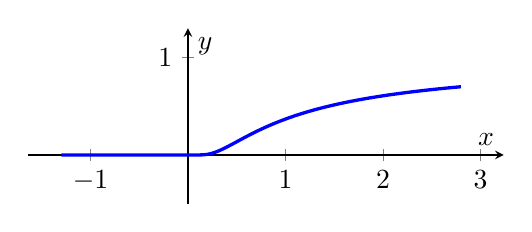
\begin{tikzpicture}[
  declare function={
    func(\x)= (\x <= 0) * (0)   +
              (\x > 0) * (e^(- 1 / \x))
   ;
  }
]
\begin{axis}[
  axis x line=middle, axis y line=middle,
  ymin=-0.5, ymax=1.3, ytick={-1,0,1}, ylabel=$y$,
  xmin=-1.6, xmax=3.2, xtick={-1,...,3}, xlabel=$x$,
  domain=-1.3:2.8,samples=200, % added
  axis equal, height=1.5in, width=3in
]

\addplot [blue,line width=1.2pt] {func(x)};
\end{axis}
\end{tikzpicture} 
    \caption{the function defined in \eqref{eq:smooth-zero-func}, which is smooth at $0$}
    \label{fig:smooth-zero-func-plt}
\end{figure}

Recall that the function \begin{equation} \label{eq:smooth-zero-func}
    f(x) = \begin{cases}
        \exp(-1/x) & \text{if }x > 0, \\
        0 & \text{if }x \leq 0.
    \end{cases}
\end{equation} is a smooth function from $\R$ to $[0,1)$; see \cref{fig:smooth-zero-func-plt}. Now for any $a < b$, consider \begin{equation}
    g(x) = \frac{f(b - x)}{f(b - x) + f(x - a)}. \label{eq:transition-func}
\end{equation} % add plot for g and h
It is clear that $g$ is smooth (the denominator is nowhere zero) and increasing on $\R$, with $g(x) = 1$ when $x \leq a$ and $g(x) = 0$ when $x \geq b$. Such a function $g$ is usually called a \df{transition function}, for the obvious reason.
\begin{figure}
    \centering
        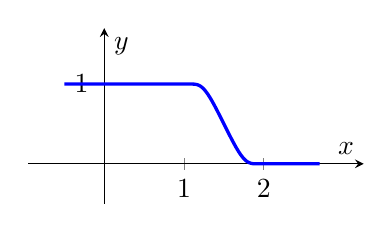
\begin{tikzpicture}[
  declare function={
    f(\x)= (\x <= 0) * (0)   +
              (\x > 0) * (e^(- 1 / \x))
   ;
   g(\x) = f(2 - \x)/(f(2 - \x) + f(\x - 1));
  }
]
\begin{axis}[
  axis x line=middle, axis y line=middle,
  ymin=-0.5, ymax=1.7, ytick={0,1}, ylabel=$y$,
  xmin=-0.7, xmax=3, xtick={0,...,2}, xlabel=$x$,
  domain=-0.5:2.7,samples=200, % added
  axis equal, height=1.5in, width=2.3in
]

\addplot [blue,line width=1.2pt] {g(x)};
\end{axis}
\end{tikzpicture} 
    \caption{the transition function defined in \eqref{eq:transition-func}, when $a = 1$ and $b = 2$}
    \label{fig:transition-func-plt}
\end{figure}

Let $0\leq a < b$, then the function $h\colon x \mapsto g(\nm{x}_2)$ is a smooth function that is $1$ on $\clos{B}(0;a)$ and $0$ outside ${B}(0;b)$. Alternatively if we define $h$ using the max norm instead of the Euclidean norm, then the closed balls should be replaced by closed cubes.
\begin{figure}
    \centering
        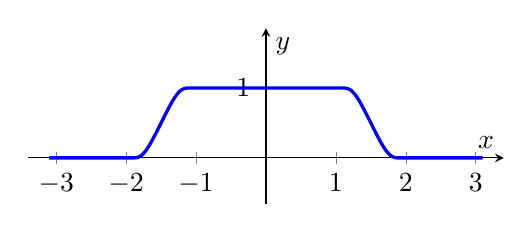
\begin{tikzpicture}[
  declare function={
    f(\x)= (\x <= 0) * (0)   +
              (\x > 0) * (e^(- 1 / \x))
   ;
   g(\x) = f(2 - \x)/(f(2 - \x) + f(\x - 1));
   h(\x) = g(abs(\x));
  }
]
\begin{axis}[
  axis x line=middle, axis y line=middle,
  ymin=-0.5, ymax=1.7, ytick={0,1}, ylabel=$y$,
  xmin=-3.4, xmax=3.4, xtick={-3,...,3}, xlabel=$x$,
  domain=-3.1:3.1,samples=400, % added
  axis equal, height=1.5in, width=3in
]

\addplot [blue,line width=1.2pt] {h(x)};
\end{axis}
\end{tikzpicture} 
    \caption{the bump function defined by $h$ in dimension $1$}
    \label{fig:smooth-bump-func-plt}
\end{figure}

The transition functions and the bump functions are very important approximants to other functions, e.g., indicator functions. The following smooth bump function also appears frequently in the literature as an approximant, because of its straightforward formula. Compose the function $x \mapsto 1 - \nm{x}^2$ with the function $f$ defined in \eqref{eq:smooth-zero-func}, we get a new smooth function \[
    \hat f(x) = \begin{cases}
        \exp\bigl(\frac{1}{\nm{x}^2 - 1}\bigr) & \text{if }\nm{x} < 1, \\
        0 & \text{if }\nm{x} \geq 1,
    \end{cases}
\] which has a closed ball/cube as its support, depending on the norm used.

We remark that $C_c^\infty(\C)$ functions must be the zero function due to Liouville's theorem, in stark contrast to the real case.

\begin{prop}[{\cite[Proposition~8.6]{folland1999}}] \leavevmode
\begin{enumerate} 
    \item $f * g = g * f$.
    \item $f * (g * h) = (f * g) * h$.
    \item $\tau_z (f * g) = (\tau_z f) * g = f * (\tau_z g)$.
    \item $\supp f * g \subseteq \clos{\supp f + \supp g}$.
\end{enumerate}
\end{prop}

In PDE theory, we are interested in functions defined on an open subset $U$ of $\R^n$; however, it can be hard to prove results directly about functions defined such $U$'s. We establish tools for functions defined on the entire $\R^n$, and then use extension and restriction arguments to specialize down to functions defined on $U$.

\cite[Proposition~4.20]{Brezis_2011} proves the second part directly

\begin{prop}[{\cite[Proposition~8.10, Exercise~8.7]{folland1999}}]
    For $f \in L^1(\R^n)$ and $g\in C^k_b(\R^n)$ (i.e., $\partial^\alpha g$ is bounded for all $\abs{\alpha} \leq k$), we have $f * g \in C^k(\R^n)$ with \[
        \partial^\alpha (f * g) = f * (\partial^\alpha g) \text{ for all } \abs{\alpha} \leq k.
    \] 

    If $f \in \locint(\R^n)$ and $g \in C_c^\infty(\R^n)$, then the same claim still holds.
\end{prop}
\begin{proof}
    The first part of theorem is really just differentiation under the integral sign of parameterized functions, \cref{cor:diff-int}.

    The second part of the theorem 
\end{proof}



\cite[Lemma~19.22]{Jost_2005}
For $f \in L^1(U)$, for any open set $V \subseteq \clos{V} \subseteq U$ and $\epsilon < \dist(V,\partial U)$, we have $f^\epsilon \in C^\infty (V)$.

Extend $f$ to $\R^n$ by defining it to be $0$ outside $U$. Then we may see $f \in L^1(\R^n)$

We now introduce the notion of a mollifier. It can smooth out functions, and allows us to approximate a given function by its smoothed-out versions.

Dividing $\hat f$ by a constant, we obtain a function $\eta \in C_c^\infty$ with $\int \eta = 1$. Define $\eta_\epsilon(x) = \frac{1}{\epsilon^n} \eta(x/\epsilon )$ for all $\epsilon > 0$. Then $\eta_\epsilon$ continues to be smooth, $\int \eta_\epsilon = 1$, and now with support contained in $\clos{B}(0;\epsilon)$. The collection $\{\eta_\epsilon\}_{\epsilon \geq 0}$ is an \df{approximation to the identity}. (converges to the Dirac delta function in the Schwartz sense) The function $\eta$ is called the \df{standard mollifier}.

Given $f\in \locint(U)$, define $f^\epsilon = f * \eta_\epsilon$ in the open set $U_\epsilon = \{x \in \R^d : \dist(x,\partial U) > \epsilon\}$.

$f^\epsilon \in C^\infty(U_\epsilon)$
$f^\epsilon \to f$ a.s.\ as $\epsilon \to 0$
uniformly on compact subsets of $U$

For any open set $U \subseteq \R^n$, $C_c^\infty(U)$ is dense in $C_c(U)$, and hence dense in $C_0(U)$.

extend $C_c^\infty(U)$ to $C_c^\infty(\R^n)$,



This tells us that the \nameref{thm:Riesz2} holds for $C_c^\infty$ test functions when the space $X$ considered is $\R^n$.

given $f \in C_c$, consider $f^\epsilon$

$C_c^\infty$ dense in $L^p$ for $1  \leq p < \infty$

% \cite[Proposition~8.17]{folland1999}

\emph{Fundamental theorem of calculus of variation}

\begin{thm}
    For $f \in \locint(U)$, if \[\int f g = 0\] for all $g \in C_c^\infty(U)$, then $f \equiv 0$ on $U$.
\end{thm}

\begin{defn}
    
\end{defn}


\subsection{Spaces of test functions}

Let $X$ be any (Hausdorff) topological space. We define $C_c(X)$ to be the space of continuous functions on $X$ with compact support. We also define $C_0(X)$ to be the space of continuous functions on $X$ such that $\{x:\abs{f(x)} \geq \epsilon\}$ is compact\footnote{The compactness stated here should be viewed as a generalization of boundedness when the space concerned does not have any metric.} for all $\epsilon > 0$.

Since $C_c$ and $C_0$ are both subsets of $C_b$, it is natural to endow the uniform norm $\nm{\blank}_u$ on the two new spaces, and we will always do this henceforth. It turns out quite naturally that $C_0(X)$, as a closed normed subspace of $C_b(X)$, is complete.

In analysis one is often interested in test function classes $C_0$ or $C_c$. Below is one reason why the choice of $C_b$ is desirable to probabilists. Suppose the sequence $\{\mu_n\} \subseteq \mathcal{P}(S)$ converges weakly to $\mu\in \M(S)$. If we take $f = 1$ on the entire $S$ in \eqref{eq:wkconv-def}, then we have $\mu(S) = \lim_n \mu_n(S) = 1$, thus proving that the weak limit $\mu$ is a Borel probability measure as well. Hence no ``mass'' is lost in this convergence, in contrast to ...

We use $\M(S)$ for the space of finite signed/complex Borel measures on $S$, $\M_+(S)$ for the space of finite positive Borel measures on $S$
\begin{defn}
    A sequence $\{\mu_n\}$ is said to 
    \begin{enumerate}
        \item \df[convergence!weak]{converge weakly} to $\mu$ if for all $f\in C_b(S)$, we have \begin{equation}
        \int_S f\,d\mu_n \to \int_S f\,d\mu, \label{eq:wkconv-def}
    \end{equation}
    which we denote by $\mu_n \wkconv \mu$;
    \item \df[convergence!vague]{converge vaguely} to $\mu$ if for all $f\in C_c(S)$, we have \begin{equation}
        \int_S f\,d\mu_n \to \int_S f\,d\mu. \label{eq:vgconv-def}
    \end{equation}
    \end{enumerate}
\end{defn}

It is common to see the notation $\mu f$ in place of $\int_S f\,d\mu$, because we may see $\mu$ as a linear operator acting on the space $C_b(S)$ with the topology of uniform convergence. The bounded continuous functions in the definition are called \df{test functions}, because this mode of convergence is tested with respect to $C_b(S)$.

Weak convergence is a subject of greater importance to probability compared to general measure theory and analysis. This has led to our choice (and many authors' choice) to present weak convergence solely in the context of probability. % A brief overview of the general theory of weak convergence has been included in \cref{sec:weak-conv-general-meas}, based on \cite{Bogachev_2018}.

If $X$ is second countable topological space, then $C_c(X)$ is separable. It follows that its uniform closure $C_0(X)$ is also separable.

Let $X$ be locally compact. If $\sup_n \nm{\mu_n} < \infty$, then it is equivalent to say $\int_S f\,d\mu_n \to \int_S f\,d\mu$ either over all $f \in C_c(X)$ or over all $f \in C_0(X)$, as a consequence of \cref{prop:strong-op-top-dense-subset}. In particular this applies to the space of subprobability measures.


loss of mass at infinity

\begin{defn}
    Let $X$ be an LCH space. A positive \df{Radon measure} $\mu$ on $X$ is a Borel measure that is locally finite, outer regular on all Borel sets, and compact inner regular on all open sets.
\end{defn}

Also may known as \emph{Borel regular measure} or \emph{Riesz measure}

\begin{prop}
    Every Radon measure is compact inner regular on $\sigma$-finite Borel sets. In particular, every $\sigma$-finite Radon measure is compact inner regular on all Borel sets.
\end{prop}

Since we are in a Hausdorff space, a compact inner regular measure is also closed inner regular, and because the measure is finite, it is also outer regular. \textcite{Bogachev_2007,Bogachev_2018} defines a signed measure to be inner regular

Indeed, for finite measures, Radon measures are the same as compact inner regular measures.

\begin{prop}
    Every locally finite Borel measure on an lcscH space is compact inner regular on all Borel sets, and is hence a Radon measure.
\end{prop}

On an lcscH spcae, finite/signed/complex Borel measures are always Radon.

Hence we may identify $\M(X)$ with the space of linear functionals on $C_c(X)$. This allows us to define the weak-star topology on $\M(X)$ by defining the convergence $\mu_n \to \mu$ in $\M(X)$ if \[
    \int f\,d\mu_n \to \int f\,d\mu \quad \text{for all }f \in C_c(X).
\] 

In notation we can write $\sigma\bigl(\M(X), C_c(X) \bigr)$

In fact, this allows us to define a weak-star topology on $\M(X)$. It is clear that $\mu_n \to \mu$ in the weak-star sense if and only if 

% \begin{namedthm}[Riesz–Markov–Kakutani theorem for compact metric spaces]
%     Let $(X,d)$ be a locally compact metric space\footnote{Every compact metric space is separable.}, then the dual space $C(X)^*$ is isometrically isomorphic to $\M(X)$, i.e., for all linear functionals $L \in C(X)^*$, there is a unique $\mu \in \M(X)$ such that \[
%         L(f) = \int_X f\,d\mu\quad \text{for all }f\in C(X);
%     \] meanwhile $\nm{L} = \nm{\mu}$.
% \end{namedthm}

\begin{namedthm}[Riesz--Markov--Kakutani theorem for positive measures] \label{thm:Riesz1}
    
\end{namedthm}

\begin{namedthm}[Riesz--Markov--Kakutani theorem for finite measures] \label{thm:Riesz2}
    Let $X$ be a locally compact metric space, then the dual space $C_c(X)^*$ is isometrically isomorphic to $\M_\mathrm{R}(X)$, i.e., for all linear functionals $L \in C_c(X)^*$, there is a unique signed/complex inner regular Borel measure $\mu$ such that \[
        L(f) = \int_X f\,d\mu\quad \text{for all }f\in C_c(X);
    \] meanwhile $\nm{L} = \nm{\mu}$.

    In particular, if $X$ is separable, then in the above statement $\M_\mathrm{R}(X) = \M(X)$; if furthermore $X$ is compact,\footnote{Compact metric spaces are obviously Lindelöf, and hence separable; see \cref{prop:2nd-count-separable-lindlof}.} then $C_c(X) = C(X)$.

    Every instance of $C_c(X)$ above can be replaced by its uniform closure $C_0(X)$.
\end{namedthm}
% https://math.stackexchange.com/questions/184766/when-is-c-0x-separable

% finite Radon measure (Bogachev 7.1)

% In particular, if $X$ is further assumed to be second countable, then the space of Radon measures $\M_r(X)$ above is just the space of Borel measures $\M(X)$.

vague limit of Radon measures is Radon, and when $\mu_n$ are all positive measures, then the vague limit $\mu$ is positive. To see this, take $f$ to be any nonnegative $C_b$ function. Then $\int f\,d\mu_{n} \to \int f\,d\mu \geq 0$, enforcing $\mu(X) \geq 0$.

\begin{cor}
    $\M_\mathrm{R}(X)$ is a closed subspace of $\M(X)$ and hence a Banach space.
\end{cor}

\begin{prop}
    In a locally compact metric space $X$ with $\mu_n \in \M_r^{+}(X)$ such that $\mu_n \to \mu$, one has $\mu(X) \leq \liminf_n \mu_n (X)$. If $\mu_n$ is allowed to be signed, then $\abs{\mu}(X) \leq \liminf_n \abs{\mu_n} (X)$.
\end{prop}

If one is familiar with Banach space theory, this is an immediate consequence of the \flcnameref{thm:unif-bdd-principle}.

\section{Fourier series}

\section{Fourier transform of functions and measures}

\section{Laplace transform}

% \section{Sobolev spaces}
% \chapter{A glimpse of Fourier analysis}

\phantomsection
\chapter*{\Large Interlude: Between Measure and Probability}
\addcontentsline{toc}{part}{Interlude}
\chaptermark{Interlude}

\part{Probability}
\chapter{Interpreting probability using measure theory}
\section{Distributions} \label{sec:dist}
From now on ($\sigma$-)algebras will be called {($\sigma$-)fields}. The measure space $(X,\A,\mu)$ will be replaced by $(\Omega,\F,P)$ with $P(\Omega)=1$, which we call a \df{probability space}. In the probability triplet $\Omega$ is called the \df{sample space}, and $\F$ is called the \df{event space}, which contains all the possible \df[event]{events}. If $\Omega$ is a countable set and $\F = \wp(\Omega)$, then the probability space is \df[discrete probability space]{discrete}.

Given an underlying measurable spaces $(\Omega,\F)$, a measurable function $X\colon (\Omega,\F) \to (S,\mathcal{S})$ is called a \df{random variable}. If $(\Omega,\F,P)$ is discrete, then the image of any function $X$ is forced to be countable. We may then let $S = X(\Omega)$ and $\mathcal S = \wp(S)$, and $X$ is obviously measurable. The random variable defined on a discrete space is called a \df{discrete random variable}, and its distribution is also \df[discrete distribution]{discrete}. If $(S,\mathcal S)$ is a measurable subspace of $(\R,\B)$, we call the random variable \df[real-valued random variable]{real-valued}. In general when $(S,\mathcal S)$ is a measurable subspace of $(\R^d,\B^d)$, then $X$ may be called a \df{real random vector}. The preference of Borel $\sigma$-field over the Lebesgue $\sigma$-field has been discussed in \cref{sec:measurable-functions}.

Given a random variable $X$, following \cref{sec:image-measure} we may define a probability measure $\mu$ on $(S,\mathcal{S})$ given by \begin{equation} \label{eq:official-prob-dist-defn}
    \mu(A) = P\bigl(X^{-1}(A)\bigr) = P(X\in A) \text{ for all }A\in \mathcal{S}.
\end{equation}
We call this the \df{probability distribution/law}\footnote{Another common notation is $\mathcal{L}$ that stands for ``law''.} of $X$, denoted by $X \sim \mu$. It characterizes how probability of (the image of) $X$ is distributed across the target space $(S,\mathcal S)$\footnote{In comparison, $P$ characterizes the \emph{underlying} space $(\Omega,\F)$.}. The $X \in A$ above is a shorthand for $\{\omega\in \Omega:X(\omega)\in A\}$, and this convention\footnote{In fact we have used this shorthand before, when discussing uniform integrability.} is widely adopted throughout probability, as long as the context is clear. It also corresponds to the intuitive understanding of a random variable $X$ as a ``variable'' taking random values by ignoring the underlying $\omega$, but we must not take this formally. When two $(S,\mathcal{S})$-valued random variables $X$ and $Y$ (on possibly different underlying spaces) have the same distribution $\mu$, we write $X \eqD Y$.

It is clear that a measure $\mu$ on a measurable subspace of $(\R,\B)$ can be naturally extended to a measure on $(\R,\B)$ (by setting all the new sets to measure $0$). Therefore it always makes sense to regard the distribution of any real-valued random variable as a Borel measure on $\R$.

\begin{rem}
    Another perspective we can take is to always let real-valued random variables take $(S,\mathcal S)$ to be exactly $(\R,\B)$. In this setup $\mu$ will always be a Borel measure. When $X$ is a random variable with $S \coloneqq X(\Omega)\subsetneq \R$, we can always consider the restriction of the distribution $\mu_X$ to $(S,\B|_S)$ to obtain our adopted definition of probability distribution in \eqref{eq:official-prob-dist-defn}. This alternative perspective is suitable for discussing distribution functions, while our previous perspective is suitable for discussing density functions, as we will see.
\end{rem}

\begin{rem}
Throughout the notes, random variables are \emph{almost always} taken to be real-valued\footnote{We have only discussed the integration of real/complex-valued functions. Some generalizations can definitely be made (to for example, Banach-valued functions/random variables), but it is beyond the scope of this survey.}. The exceptions should be noted by the readers on their own.
\end{rem}

The \df[cumulative distribution function@(cumulative) distribution function]{(cumulative) distribution function} (c.d.f.)\ of a real-valued random variable $X$ is defined to be a function $F\colon \R \to [0,1]$ given by \[
    F(x) = P(X \leq x) = \mu(-\infty,x].
\]
Again we mention that the choice of ``$\leq$'' instead of ``$<$'' in the definition of distribution function is a convention. In fact going back to Kolmogorov's original \textit{Foundations of the Theory of Probability}, the distribution function is defined by $P(X < x)$.

We now slightly modify \cref{thm:increasing-rcont-Borel-measure-connection}\ref{enu:CDF-measure}\ref{enu:measure-CDF} to suit our purpose. Note now we instead start with the original part~\ref{enu:measure-CDF}.
\begin{thm} \label{thm:measure-CDF-prob}
    Let $X$ be a real-valued random variable with distribution $\mu$ on $(\R,\B)$, then its distribution function $F$ has the following properties:
        \begin{itemize}
            \item $\lim_{x \to -\infty} F(x) = 0$ and $\lim_{x \to \infty} F(x) = 1$;
            \item it is increasing and right-continuous; 
            \item it has left limits in the sense that \[
                F(x-) = \lim_{y \to x^-} F(y) = \mu(-\infty,x),
            \] which also implies $\mu\{x\} = F(x) - F(x-)$.
        \end{itemize}
\end{thm}
Since $\mu$ is now a probability measure, the first bullet point follows directly. The rest has been proved already before. We remark also that every distribution function has countably many discontinuities (by \cref{prop:discont-countable}), and is hence continuous a.e.

Recall \cref{thm:increasing-rcont-Borel-measure-connection}\ref{enu:CDF-measure}. We can slightly modify its statement and proof to get the version for obtaining a unique Borel probability measure.

\begin{thm} \label{thm:CDF-measure-prob}
    Conversely, let $F\colon \R\to [0,1]$ be an increasing, right-continuous function with \[
        \lim_{x \to -\infty} F(x) = 0\quad \text{and} \quad \lim_{x \to \infty} F(x) = 1,
    \] then there is a unique probability measure $\mu$ on $(\R,\B)$ such that \[
        \mu(-\infty,x] = F(x) \quad \text{for all }x\in \R.
    \]
\end{thm}

\Cref{thm:CDF-measure-prob} tells us that as long as we have the distribution function of a random variable $X$, which increases from $0$ to $1$ and is right-continuous, then the distribution function determines the distribution of the random variable. Formally we are now ready to state 
\begin{cor} \label{cor:dist-cdf-equiv}
    For two real-valued random variables $X$ and $Y$, we have $F_X = F_Y$ if and only if $\mu_X = \mu_Y$, i.e., a one-to-one correspondence between distribution functions and distributions.
\end{cor}

This observation is very fundamental because it tells us we can see the distribution of a real random variables from two distinct perspectives. The corollary further suggests that given a random variable, we may specify its distribution solely in terms of a function $F\colon \R \to [0,1]$ that is increasing, right-continuous, with \[
        \lim_{x \to -\infty} F(x) = 0\quad \text{and} \quad \lim_{x \to \infty} F(x) = 1.
\] We call such a function $F$ a \df[cumulative distribution function@(cumulative) distribution function]{(cumulative) distribution function} on its own. And we write $X \sim F$ if $X \sim \mu_F$, the unique probability measure associated to the distribution function $F$.

\begin{thm} \label{thm:cdf-unif-identification}
    Indeed any distribution function $F \colon \R \to [0,1]$ can be realized as the distribution function of some real random variable $X$ on some probability space $(\Omega,\F,P)$. In particular we can take the probability space to be $([0,1],\B_{[0,1]},m)$, and realize $X \sim F$ from a $\Unif[0,1]$ random variable on this probability space.
\end{thm}
\begin{proof}[First construction]
    By \cref{thm:CDF-measure-prob}, we know every distribution function $F$ gives rise to a unique probability measure $\mu$ on $(\R,\B)$. Now let $(\Omega,\F,P) = (\R,\B,\mu)$ and let $X$ be the identity map on $\R$.
\end{proof}
Given one knows \cref{thm:CDF-measure-prob}, this first proof is indeed a very trivial construction. The second proof, independent of \cref{thm:CDF-measure-prob}, is more interesting and certainly of significance to us.
\begin{proof}[Second construction]
    Let $(\Omega,\F,P) = ([0,1],\B_{[0,1]},m)$, and we define \begin{equation}
        X(\omega) = \inf\{y : F(y) \geq \omega\} \coloneqq F^{-1}(\omega). \label{eq:dist-func-inv-def}
    \end{equation}
    It is clear to see that $X(\omega) \leq y$ if and only if $\omega \leq F(y)$. Therefore for all $y\in \R$, \[
        P(X \leq y) = P\bigl(\omega\leq F(y)\bigr) = F(y).
    \]
    The construction still works out perfectly if one replaces $\omega$ by $U(\omega)$, where $U \sim \Unif[0,1]$. This is because the identity map is the special case of a $\Unif[0,1]$ random variable. We conclude that we can use any $\Unif[0,1]$ random variable $U$ to generate a $\mu$-distributed random variable on the probability space $([0,1],\B_{[0,1]},m)$, via the recipe $F_\mu^{-1}(U)$.
\end{proof}

The realization of $X\sim F$ described above will play a pivotal role later in \cref{sec:indep-seq}.

There are several things we need to mind here. Firstly, one can show that $\inf\{y : F(y) \geq \omega\} = \sup\{y : F(y) < \omega\}$. The ``$\geq$'' direction is obvious. To see the ``$\leq$'' direction, consider any $x > \sup\{y : F(y) < \omega\}$. It is clear that $F(x) \geq \omega$, and thus by right-continuity we have $F(\sup\{y : F(y) < \omega\})\geq \omega$. Note that we have also just proved that the infimum in \eqref{eq:left-cont-inv} can be attained.    

Secondly, the $X$ defined here in \eqref{eq:dist-func-inv-def} is sometimes called the \df{generalized inverse/quantile function} of the distribution function $F$, denoted by $F^{-1}$. Distributions functions are not in general invertible, but this almost invertibility between $\R$ and $[0,1]$ motivates our definition.

We now show $X(\omega)$ is continuous from the left, i.e., for all $a \in (0,1]$, \begin{equation}
    \lim_{\omega \to a^-} X(\omega) = X(a) \label{eq:left-cont-inv}.
\end{equation} Since $F$ is increasing, the limit exists and the ``$\leq$'' direction follows. Now suppose we have the strict inequality ``$<$''. This implies $F\bigl(\lim_{\omega \to a^-} X(\omega)\bigr) < a$. Since $F\bigl(X(\omega)\bigr) \geq \omega$, we get a contradiction. Hence we have the equality in \eqref{eq:left-cont-inv}.

Thirdly, we remark that $\ol{X}(\omega) = \sup\{y:F(y)\leq \omega\} = \inf\{y:F(y) > \omega\}$ has the same distribution as our $X$ defined in \eqref{eq:dist-func-inv-def}. In fact $X$ and $\ol{X}$ differ at countably many points; $X(\omega) \neq \ol{X}(\omega)$ if and only if $X([0,\omega]) - X\bigl([0,\omega)\bigr)$, i.e., there is a jump for $X$ at $\omega$. For distinct $\omega\in [0,1]$ these intervals have to be disjoint, and hence there are only countably many such intervals. The proof of this final step is included in \cref{prop:discont-countable}. We leave it as an exercise to reader to show that this $\ol{X}$ is right-continuous. (This will be used in the proof of \cref{lem:Helly-pre}, when constructing a right-continuous candidate for a distribution function.)

We will generalize this result later. Generalization of \cref{thm:cdf-unif-identification}
\begin{thm}[{\cite[Exercise~8.3.4]{Cohn_2013}}]
    
\end{thm}

Let $X\colon (\Omega,\F)\to (S,\mathcal S)$ have distribution $\mu$, and the codomain $(S,\mathcal S)$ has a natural underlying measure $\rho$ with $\mu \ll \rho$. The \df[probability density function@(probability) density function]{(probability) density function} (p.d.f.)\footnote{or \emph{frequency function}} of the random variable $X$ is Radon--Nikodym derivative $d\mu/d\rho$ of the probability distribution with respect to this underlying measure for the image space.

Specifically, when $X$ is a discrete random variable, then the counting measure is a natural measure for $(S,\mathcal S)$, and obviously $\mu \ll \mathrm{count}$. Hence $d\mu/d(\mathrm{count})\colon x \mapsto \mu\{x\}$ is the density function, which is also called the \df{probability mass function} (p.m.f.)\footnote{to emphasize we are in the discrete setting}.

On the other hand, recall \cref{fact:restrict-meausre-restrict-space}. Given a random variable $X$, if the codomain $S$ is a Borel subset of $\R^d$ and $\mathcal S = \B^d|_S$, and in addition $\mu \ll m|_S$, then $d\mu/d(m|_S)$ is the density function. We call such $X$ a \df{continuous random variable}\footnote{The term ``continuous'' here refers to the absolute continuity of the distribution function, and does not require that the density function must be continuous.}. Note in this continuous case the density function is a.e.\ defined, but in the discrete case the density (p.m.f.)\ is exact. Later on when discussing continuous random variables, we usually only write out the case $(S,\mathcal{S}) = (\R,\B)$ for brevity, since the density function $d\mu / d(m|_S)$ defined on $S$ can be naturally extended to the entire $\R$.

The definition of density function for a continuous random vector is the same as above, with the Lebesgue measure replaced by the product Lebesgue measure. Also notice that the product of counting measures on marginal spaces is the counting measure on the product space, so we do not need to make a separate note for p.m.f.\ when $(S,\mathcal S)$ is a product of discrete spaces. In contrast to distribution functions which are only nice to work with in dimension $1$, density functions is defined for general random vectors in $\R^d$, as long as $\mu \ll m$.

We can define the class of distributions with densities solely in terms of their density functions. When the desired distribution of $X$ is discrete, it is clear that we can specify this distribution using a \df{probability mass function} (on its own), i.e., a function $p\colon X(\Omega) \to [0,1]$ such that \[\sum_{x\in X(\Omega)} p(x) = 1.\] When the desired distribution of $X$ is continuous, then a nonnegative Borel measurable function $f$ satisfying \[
    \int_\R f(x)\,dx = 1,
\] called a \df[probability density function@(probability) density function]{(probability) density function} (on its own) will specify the distribution. In summary, probability mass and density functions let us generate discrete and continuous random variables.


\section{Moments, independence, and joint distributions} \label{sec:moment-indep-joint}

\subsection{Expectations as integrals}

The average value of function

Following the theory of Lebesgue integration we have developed, 

\begin{defn}
    Let $X$ be a nonnegative random variable, its \df{expectation/expected value} is given by \[
    \E X = \int_\Omega X\,dP.
    \]
    
    If $X$ is a signed real-valued random variable, with one of $\E X^+$ and $\E X^-$ being finite, then we can define the \emph{expectation} of $X$ to be \[
        \E X = \int_\Omega X\,dP = \E X^+ - \E X^-.
    \]
    In particular, when $\E \abs X < \infty$\footnote{One often prefers to write $\E\abs{X} < \infty$ for integrability of $X$ in probability. However, when we are dealing integration with respect to two different measures, then the $L^1$ notation should again be helpful.}, $\E X$ always exists. This is the case we are interested in mostly.
\end{defn}

Since the distribution $\mu$ on $(S,\mathcal{S})$ is given as the image measure $P\circ X^{-1}$, by \cref{prop:image-meas-cov} we have for $g\colon (S,\mathcal S) \to (\R,\B)$, if $g \geq 0$ or $g\circ X \in L^1(\Omega)$, then \[
    \E g(X) = \int_\Omega g\bigl(X(\omega)\bigr)\,dP(\omega) = \int_S g(x) \,d\mu(x).
\] In particular, if $X$ is real-valued, then \[
    \E X = \int_\Omega X(\omega)\,dP(\omega) = \int_S x\,d\mu(x).
\] Furthermore, if $X$ is discrete, then \[
    \E X = \sum_{x \in S} x \mu\{x\}; 
\] and if $X$ is continuous with density $f$, then \[
    \E X = \int x f(x)\,dx
\]

It should be clear that $X =_d Y$ (on possibly different probability spaces), then $\E X = \E Y$.

\begin{namedthm}[Cauchy--Schwarz inequality] \label{thm:c-s-ineq-prob} For any random variables $X$ and $Y$, 
    \[\E \abs{XY} \leq \bigl(\E X^2\bigr)^{1/2} \bigl(\E Y^2\bigr)^{1/2}\]
\end{namedthm}

\begin{namedthm}[Jensen's inequality] \label{thm:Jensen-prob}
    Let $\E\abs X <\infty$. Suppose $I$ is an interval containing the range of $X$, and we have a convex function $\phi\colon I\to \R$. Then \[
        \phi(\E X) \leq \E \phi(X).
    \]
\end{namedthm}
    
\begin{namedthm}[Lyapunov's inequality]
For $1 \leq p \leq q <\infty $, we have $(\E\abs{X}^p)^{1/p} \leq (\E \abs{X}^q)^{1/q}$.

It follows directly that \[L^1 \supseteq L^2 \supseteq \dotsb \supseteq L^\infty.\]
\end{namedthm}

However, $L^\infty \neq \bigcap_{p=1}^\infty L^p$. The Gaussian measure is the counterexample.

\subsection{Independence, a new measure-theoretic notion}

\begin{defn}
    We say events $A_1,\dotsc,A_n \in \F$ are \df[independent!events]{independent} if for every subcollection $J \subseteq [n]$, \[
    P\biggl(\bigcap_{j\in J} A_j\biggr) = \prod_{j\in J} P(A_j).
\] % An infinite collection of events $A_\alpha$ ($\alpha \in I$) are \emph{independent} if any finite subcollection of the $A_\alpha$'s are independent.
Collections of events $\A_1,\A_2,\dotsc,\A_n$ are \df[independent!collections of events]{independent} if for every subcollection $J \subseteq [n]$, \[
    P\biggl(\bigcap_{j \in J} A_j\biggr) = \prod_{j\in J}P(A_j)
\] for all possible $A_j \in \A_j$ ($j \in J$).
Random variables $X_1,X_2,\dotsc,X_n$ are \df[independent!random variables]{independent} if $\sigma(X_1),\dotsc,\sigma(X_n)$ are independent collections of events.

When the number of events/collection of events/random variables are infinite, then events/collection of events/random variables are said to be \emph{independent} if every finite subcollection of these events/collection of events/random variables satisfies their independence definitions given above.
\end{defn}

We will be concerned mostly with the finite collection in this section. Their extension to be infinite case should be easy.

\begin{prop}
    The following statements are equivalent.
    \begin{enumerate}
        \item $A_1,A_2,\dotsc,A_n$ are independent;
        \item $A_1^\cpl,A_2,\dotsc,A_n$ are independent;
        \item $\ind_{A_1},\ind_{A_2},\dotsc,\ind_{A_n}$ are independent.
    \end{enumerate}
\end{prop}

Given $(\Omega,\F,P)$, and let $X$ and $Y$ be two random variables taking values on $(S_1,\mathcal S_1)$ and on $(S_2,\mathcal S_2)$ respectively, with distributions $\mu_X$ and $\mu_Y$. The \df{joint distribution} $\mu_{X,Y}$ of the pair $(X,Y)$ is given by \[
    \mu_{X,Y}(A) = P\times P\bigl((X,Y) \in A\bigr)\quad\text{for all }A\in \mathcal{S}_1\otimes\mathcal{S}_2.
\] The $P\times P$ here is a product probability measure on $(\Omega\times \Omega, \F\otimes \F)$.

The definition of joint distributions can obviously be generalized to any finite and countably infinite number of random variables, by our previous discussions on product measure spaces.

\begin{thm}[(independence characterizations)] \label{thm:indep-char}
    For two random variables $X$ and $Y$ taking values in $(S_1,\mathcal S_1)$ and $(S_2,\mathcal S_2)$ respectively, the following are equivalent characterization that $X$ and $Y$ are independent (which we sometimes denote by $X \perp Y$).
    \begin{enumerate}
        \item $P(X\in A_1)P(Y \in A_2) = P(X \in A_1, Y\in A_2)$ for all $B_1\in \mathcal S_1$ and $B_2\in \mathcal S_2$;
        \item \label{enu:indep-prod-meas} $\mu_X \times \mu_Y = \mu_{X \times Y}$;
        \item $P(X\in A_1)P(Y \in A_2) = P(X \in A_1, Y\in A_2)$ for all $A_1\in \mathcal K_1$ and $A_2\in \mathcal K_2$, where $\mathcal K_1$ and $\mathcal K_2$ are two $\pi$-systems such that $\mathcal S_1 = \sigma(\mathcal K_1)$ and $\mathcal S_2 = \sigma(\mathcal K_2)$;
        \item \label{enu:indep-check-via-L2} for all $f(X), g(Y) \in L^2$, \[
            \E[f(X)g(Y)] = \E f(X)\E g(Y).
        \] Here the $L^2$ requirement is a sufficient condition for us to assert the integrability of $f(X)g(Y)$, by \nameref{thm:c-s-ineq-prob}.
    \end{enumerate}
\end{thm}

\begin{proof}
    Recall that the product measure is the unique extension of the product of marginal measures on measurable rectangles.
\end{proof}

\begin{prop}
    A real-valued random variable $X$ independent of itself must take a constant value a.s.
\end{prop}

If we know $X \in L^2$, then the result is immediate: by part~\ref{enu:indep-check-via-L2} above we have $\E X^2 = (\E X)^2$, which implies $\Var(X) = 0$, i.e, $X = \E X$ a.s. But there is no need to make the $L^2$ assumption.

\begin{proof}
    For any $A\in \mathcal B$, we have \[
    	P(X\in B)P(X\in B) = P(X \in B),
    \] which implies $P(X \in B) = 0$ or $1$.
	
    We now prove a more general claim that directly implies the proposition: 
    \begin{quote}
        a $\{0,1\}$-valued Borel probability measure $\mu$ on a separable metric space $S$ must be a point mass.\footnote{Hence the ``real-valued random variable $X$'' in the proposition statement may be replaced by ``random variable $X$ taking values in a separable metric space''.}
    \end{quote}
    We know every open cover has a countable subcover in $S$ (this is \cref{prop:2nd-count-separable-lindlof}). Fix $\epsilon >0$ and consider the $\epsilon$-balls $B(x;\epsilon)$ around each $x\in S$. Now we can choose a countable subcollection $\{B(x_j;\epsilon)\}_{j=1}^\infty$ that covers $S$, and this implies there exists one unique $j\in \N$ such that $\mu\bigl(B(x_j;\epsilon)\bigr) = 1$. We call this ball $B_\epsilon$.

    The intersection of any two such balls $B_{\epsilon_1}\cap B_{\epsilon_2}$ must have measure $1$. This is because if it has measure $0$, then $B_{\epsilon_1} - B_{\epsilon_2}$ and $B_{\epsilon_2} - B_{\epsilon_1}$ both have measure $1$ despite being disjoint. Let $\epsilon_n = 1/n$, and it follows that \[
        \mu\biggl(\bigcap_{n=1}^\infty B_{1/n}\biggr) = \lim_{k\to \infty} \mu\biggl(\bigcap_{n=1}^k B_{1/n}\biggr) = 1.
    \] Since $B\coloneqq \bigcap_{n} B_{1/n}$ has diameter $0$, $B$ is a singleton set of measure $1$.

    One has to be amazed that for any choice of countable subcover of open balls above, the end product is always \emph{the} unique singleton set. (When $S = \R^d$ we can let these balls be $2^{-n}$-cubes, whose countable disjoint union is the entire space.)
\end{proof}

As a consequence of Fubini--Tonelli, for Borel measurable $g\colon S_1\times S_2 \to \R$ such that $g \geq 0$ or $\E \abs{g(X,Y)} < \infty$, we have \begin{align*}
        \E g(X,Y) & = \int_{\R^2} g(x,y)\,d(\mu_X \times \mu_Y) \\ & = \int_{\R}\int_{\R} g(x,y)\,d\mu_X \,d \mu_Y.
    \end{align*}


marginal density
\begin{prop}[(Factorization)]
    Let $X$ and $Y$ be two discrete/continuous random variables. Then $X$ and $Y$ are independent if and only if for all $x,y\in \R$,
    \begin{enumerate}
        \item \label{enu:factor-density} $f_{X,Y}(x,y) = f_X(x)f_Y(y)$, where the $f$'s are density functions;
        \item \label{enu:factor-arbitrary} $f_{X,Y}(x,y) = g(x) h(y)$ for some functions $g$ and $h$.
    \end{enumerate} To be precise the equalities above are up to measure zero.
\end{prop}
\begin{proof}
    We show the case when $X$ and $Y$ are continuous random variables on $\R$. For all $A_1,A_2\in \B$, we have \begin{align*}
        \mu_{X,Y}(A_1 \times A_2) & = \int_{A_1 \times A_2} f_{X,Y}(x,y)\,dx\,dy, \\
        \mu_X(A_1) \times \mu_Y(A_2) & = \int_{A_1}f_X(x)\,dx \int_{A_2} f_Y(y)\,dy \\ & = \int_{A_1} \int_{A_2}f_X(x)f_Y(y)\,dx\,dy.
    \end{align*}
    Part~\ref{enu:factor-density} now follows easily. To see the ``if'' direction of part~\ref{enu:factor-arbitrary}, integrate both sides of $f_{X,Y}(x,y) = g(x) h(y)$ over $A_1 \times A_2$, we have \[
        \mu_{X,Y}(A_1 \times A_2) = \int_{A_1} g(x)\,dx \int_{A_2} h(y)\,dy.
    \] Consider $C = \int_{\R} h(y)\,dy$. We may divide $h$ by this constant $C$ and multiply $g$ by this $C$, and assume without loss of generality that \begin{align*}
        \mu_X(A_1) = \mu_{X,Y}(A_1\times \R) = \int_{A_1} g(x)\,dx, \\
        \mu_Y(A_2) = \mu_{X,Y}(\R \times A_2) = \int_{A_2} h(y)\,dy.
    \end{align*} This completes the proof.
\end{proof}

\begin{defn}
    The \df{variance} of an $L^2$ random variable $X$ is defined by \begin{align*}
    \Var(X) & = \E(X - \E X)^2 \\
    & = \E (X^2) - 2 \E X\cdot \E X + (\E X)^2 \\
    & = \E(X^2) - (\E X)^2.
    \end{align*}
    Given two $L^2$ random variables $X$ and $Y$, their \df{covariance} is defined by\begin{align*}
        \Cov(X,Y) & = \E\bigl((X - \E X)(Y - \E Y)\bigr) \\
        & = \E (XY) - \E X \cdot \E Y;
    \end{align*} they are said to be \df{uncorrelated} if $\Cov(X,Y) = 0$, i.e., 
    \[\E X \cdot \E Y = \E(XY);\] and their \df{correlation} is defined by \[
    	\Corr(X,Y) = \frac{\Cov(X,Y)}{\sqrt{\Var(X)\Var(y)}}.
    \]
    
\end{defn}

As mentioned perviously, the $L^2$ requirement is a sufficient, but not necessary condition for covariance to always exist. This is similar to the $L^1$ requirement sufficient for the expectation of a random variable to always exist.

Let $A$ and $B$ be two events and consider two indicators $\ind_A$ and $\ind_B$. Notice \[
    \Cov(\ind_A,\ind_B) = \E(\ind_{A\cap B}) - \E\ind_{A} \E\ind_{B} = P(A\cap B) - P(A) P(B).
\]
We say $A$ and $B$ are \df{positively correlated} if the covariance above is $\geq 0$, i.e., $P(A\cap B) \geq P(A) P(B)$, or equivalently $P(A \giv B) \geq P(A)$. We say $A$ and $B$ are \df{negatively correlated} if the $\geq$'s are replaced by $\leq$'s. Note that the covariance and correlation are symmetric.

\subsection{Sum of independent random variables}
Fourier transform

The \df[tail sigma-field@tail $\sigma$-field]{tail $\sigma$-field} of a sequence of random variables $X_1,X_2,\dotsc$ to be \[
    \mathcal{T} = \bigcap_{n=1}^\infty \sigma(X_n,X_{n+1},\dotsc).
\]

Let $\pi\colon \N \to \N$ be a map such that $\pi(n) = n$ for all $n$ larger than some finite $M$, which means that $\pi$ only permutes finitely many indices. We call such a map a finite permutation of $\N$.

$\omega = (\omega_1,\omega_2,\dotsc)$, $\omega_j = X_j(\omega)$, the random variables $X_j$ works as projection maps, and we have identified random variables with the coordinates of the samples (in our constructed product space).

An event is \df{permutable} if $\pi^{-1}A = \pi\{\omega:\pi \omega \in A\}$ for all finite permutations, which means exactly that an event remains invariant when we exchange the order of finitely many random variables.

\begin{namedthm}[Kolmogorov zero--one law] \label{thm:K-01-law}
    Let $X_1,X_2,\dotsc$ be a sequence of independent random variables, then any event in its tail $\sigma$-field $\mathcal T$ has probability $0$ or $1$.
\end{namedthm}

\begin{namedthm}[Hewitt--Savage zero--one law] \label{thm:HS-01-law}
    Let $X_1,X_2,\dotsc$ be a sequence of i.i.d.\ random variables, then any event in its exchangeable $\sigma$-field $\mathcal E$ has probability $0$ or $1$.
\end{namedthm}

% p264 Klenke

exchangeable family of random variables

\begin{prop}
    
\end{prop}

\section{Basic concentration and deviation inequalities}
We begin with the vanilla Markov's inequality that imposes minimal assumptions on the distribution of the random variable $X$ considered.
\begin{namedthm}[Markov's inequality] \label{thm:Markov-ineq-prob}
    Let $0< p < \infty$. For any $a > 0$, we have \[
        P(\abs X \geq a) \leq \frac{1}{a^p} \E(\abs X^p).
    \]

    In particular, for nonnegative $X$, we have \[
        P(X \geq a) \leq \frac{\E X}{a}.
    \]
\end{namedthm}

These are just special cases of the following specialized version.

\begin{namedthm}[Generalized Markov's inequality]
    Let $\phi\colon \R \to [0,\infty)$ be increasing. Then for any random variable $X$, and any $a\in \R$ with $\phi(a)\neq 0$, we have \[
        P(X \geq a) \leq \frac{1}{\phi(a)}\E \phi(X).
    \]
\end{namedthm}

In probability theory it is often useful to take this $\phi$ to be an exponential function. If we assume $\E \exp(X) < \infty$, we get tail probabilities that are exponentially decreasing in $a$. In fact, the derivation of many concentration inequalities depends in general on a technique called \emph{Chernoff method}, where you set $\phi(x) = \exp(\lambda x)$, and in the end you aim to minimize \[\frac{1}{\exp(\lambda a)}\E \exp(\lambda X) \] over all $\lambda \in \R^{>0}$ (so that $\phi$ is increasing).

Unfortunately $\E \exp(\lambda X)$ can be infinite, in particular for $X$ with heavy-tailed distributions. For random variables with tails thinner than exponential or Gaussian random variables, the Chernoff method provides us valuable insights. Such random variables are known as \df[subexponential random variable]{subexponential} and \df[subguassian random variable]{sugaussian random variables}, and with information about its tail behavior, or equivalently, $\E \exp(\lambda X)$, we can derive much better concentration bounds than the vanilla \nameref{thm:Markov-ineq-prob} (and its consequences). See \cite{Vershynin_2018} and \cite{Handel2014HDP} for the study of these concentration results, and their applications.

The exponential and Gaussian random variables represent the two canonical tail behavior of a random variable. To get this idea, we will let the reader verify that $\E \exp(\lambda X) = \frac{\rho}{\rho - \lambda}$ for $X \sim \Exp(\rho)$ and $\lambda < \rho$; and also $\E\exp(\lambda Y) = \exp(\lambda^2 / 2)$ for $Y \sim N(0,1)$.

The transform $\E\exp(\lambda X)$ of the random variable $X$ is called the \df{moment generating function} of $X$, denoted by $M_X(\lambda)$. Apart from its significance in proving concentration bounds, it also recovers the distribution of $X$, which we will study later. We will also see that under suitable conditions for $\lambda$, if $M_X(\lambda) < \infty$, then $X \in L^p$ for all $p \in [1,\infty)$. This is expected by considering the Taylor expansion of the exponential function. 

Going back to vanilla \nameref{thm:Markov-ineq-prob}, we have the moment bound \[
    P(\abs X \geq a) \leq \inf_{p\in \N} \frac{1}{a^p} \E(\abs X^p),
\] which is in fact always as least as good as the Chernoff bound. However, the optimization over $p\in \N$ (or $p \in \R$) is hard to materialize.

\begin{namedthm}[Chebyshev's inequality] \label{thm:Chebyshev-ineq}
    For $X$ with $\E X^2 < \infty$, we have for all $t > 0$ that \[
        P(\abs{X - \E X} \geq t) \leq \frac{\Var(X)}{t^2}.
    \]
\end{namedthm}

\nameref{thm:Markov-ineq-prob} gives an upper bound on the tail probability, with the first moment $\E X$. A lower bound can also be obtained, with in addition the second moment $\E X^2$.

\begin{namedthm}[Paley--Zygmund inequality] \label{thm:PZ-ineq}
    Let $X \geq 0$ with $\E X^2 < \infty$. For any $0\leq \theta\leq 1$, we have \[
        P(X > \theta \E X) \geq (1-\theta)^2 \frac{(\E X)^2}{\E X^2}.
    \]
\end{namedthm}
\begin{proof}
    The case for $\theta = 1$ is trivial. We will fix $0 < \theta < 1$ first.

    The key is to use \nameref{thm:c-s-ineq-prob}: \begin{align*}
        \E X & = \E (X \ind\{X \leq \theta \E X\}) + \E(X \ind\{X > \theta \E X\}) \\
        & = \theta \E X + \sqrt{\E X^2 P(X > \theta \E X)},
    \end{align*} and then rearrange to get the desired expression.

    Now let $\theta_n = 1/n$ and take $n \to \infty$ to get the case for $\theta = 0$.
\end{proof}

We remark \nameref{thm:Markov-ineq-prob} and \nameref{thm:PZ-ineq} are related respectively to the \emph{first} and the \emph{second moment method} in probabilistic combinatorics; see \cite[Chapter~2]{Roch_2024}.



\begin{namedthm}[Hoeffding's inequality] \label{thm:Hoeffding-ineq}
    Suppose $X_{1},\ldots,X_{n}$ are independent,
    where $X_{k}$ is almost surely contained in $[a_{k},b_{k}]$ with
    means $\mu_{k}$ for all $k\in[n]$. Then for any $t\geq0$, we have
    \[
        P\biggl(\sum_{k=1}^{n}(X_{k}-\mu_{k})\geq t\biggr)\leq\exp\biggl(-\frac{2t^{2}}{\sum_{k=1}^{n}(b_{k}-a_{k})^{2}}\biggr).
    \]
\end{namedthm}

Judging by the look of the above inequality, it is clear that we need the Chernoff method for a proof. An additional ingredient is the following well-known lemma, which is surprisingly hard to establish.

\begin{namedthm}[Hoeffding's lemma] \label{lem:Hoeffding}
    For a mean zero random variable $Y$ that is a.s.\ bounded within $[a,b]$, we have \begin{equation}\label{eq:hoeffding-lem}
        M_Y(\lambda) = \E\exp(\lambda Y) = \exp\biggl(\frac{\lambda^2 (b - a)^2}{8}\biggr)
    \end{equation}
\end{namedthm}
\begin{proof}
Since $e^{\lambda x}$ is convex, we have for $x \in [a,b]$ \[
e^{\lambda x} \leq \frac{b-x}{b-a}e^{\lambda a} + \frac{x-a}{b-a}e^{\lambda b}.
\]
Taking expectation on both sides, and we have \begin{equation}
\E \exp(\lambda Y) \leq \frac{b}{b-a} e^{\lambda a} - \frac{a}{b-a} e^{\lambda b} = e^{L(\lambda(b-a))}, \label{eq:conv-bd-mgf}
\end{equation}
where for all $h \in \R$, $L(h) = - \gamma h + \log(1 - \gamma + \gamma e^h)$, with $\gamma = -\frac{a}{b - a} > 0$ (so that the log is well-defined).

Notice that $L(0) = 0$, and $L'(0) = -\gamma + \frac{\gamma e^h}{1 - \gamma + \gamma e^h}\big\vert_{h = 0} = 0$. \begin{align*}
L''(h) & = \biggl(\frac{\gamma e^h}{1 - \gamma + \gamma e^h}\biggr)' \\
& = \frac{\gamma e^h}{1 - \gamma + \gamma e^h} - \frac{\gamma^2 e^{2h}}{(1 - \gamma + \gamma e^h)^2} \\
& = t - t^2 \leq 1/4\quad \text{for any }t\in \R, 
\end{align*}
where we let $t = \frac{\gamma e^h}{1 - \gamma + \gamma e^h}$. Now we appeal to Taylor's theorem: for $h \neq 0$, there exists a $\xi$ between $h$ and 0 such that \[L(h) = 0 + 0\cdot h + \frac{L''(\xi)}{2} \cdot h^2 \leq \frac{1}{8} h^2.\] Now let $h = \lambda(b-a)$ and plug it back into \eqref{eq:conv-bd-mgf}, and we have shown \eqref{eq:hoeffding-lem}.    
\end{proof}

At the moment, proving \nameref{thm:Hoeffding-ineq} rigorously is left as an exercise to the reader. In fact, later when studying martingales, we will prove a renowned generalization known as \nameref{thm:Azuma-Hoeffding}, and the above inequality will become a trivial special case.\footnote{Hence one may extract a proof of the above inequality from there.}

tight consider any binary random variables, with probabilities $1/2$



\section{Miscellaneous but crucial facts and tools}
\begin{defn}
    Fix the dimension $d$. The \df{standard Gaussian measure} on $\R^d$ is the measure $\gamma\colon \B(\R^d) \to [0,\infty]$ given by \[
        \gamma(A) = \frac{1}{\bigl(\sqrt{2\pi}\bigr)^d} \int_A \exp\bigl(\nm{x}^2_2 \big/ 2\bigr)\,dx.
    \]
\end{defn}

It is quite clear that $m$ and $\gamma$ are equivalent measures, since $\exp(\blank)$ is nonnegative. In fact, this crucial fact allows us to prove some deterministic facts in analysis, e.g., the space of all $n$-by-$n$ matrix, when embedded into $\R^{n^2}$, is a.e.\ invertible.

\begin{fact}
    For $Z \sim N(0,1)$, we have \[
        \E[Z f(Z)] = \E f'(Z),
    \] when the expectations on the two sides are defined.
\end{fact}

\begin{prop}[{\cite[Proposition~2.1.2]{Vershynin_2018}}\ {\cite[Lemma~12.9]{Morters_Peres_2010}}]
    For $Z \sim N(0,1)$, we have the following tail estimate: for any $t > 0$, it holds that \[
        \frac{t}{t^2+1} \frac{1}{\sqrt{2\pi }} \exp(-t^2 / 2) \leq P(X \geq t) \leq \frac{1}{t} \frac{1}{\sqrt{2\pi }} \exp(-t^2 / 2).
    \]
\end{prop}

Let $Z \sim N(0,1)$, then in general for all $k \in \N$, \[
    \E Z^{2k - 1} = 0\quad \text{and}\quad \E Z^{2k} = \frac{(2k)!}{2^k k!}.
\]

\begin{prop}
For a sequence of normal random variables $Z_n \sim N(\mu_n, \sigma_n^2)$. Suppose $Z_n \wkconv Z$, then $Z \sim N(\lim_n \mu_n, \lim_n \sigma_n^2)$.

If $Z_n \to Z$ in probability (so they live in the same probability space), then $Z_n \to Z$ in $L^p$ for all $p$.
\end{prop}

\begin{proof}
    
\end{proof}


Bogachev Theorem 1.4.3.

The coordinates of a normal random vector are independent if and only if they are uncorrelated.

Gaussian measures are orthogonally invariant. However, it is not translation invariant.

\begin{namedthm}[Gaussian isoperimetric inequality]
    
\end{namedthm}

We now restate \nameref{thm:BorelCantelli-meas-th}.

\begin{namedthm}[Borel--Cantelli lemma I] \label{thm:BorelCantelli-1-prob}
    For events $A_1,A_2,\dotsc$, if $\sum_n P(A_n) < \infty$, then \[
        P(A_n \text{ i.o.}) = 0.
    \]
\end{namedthm}

In probability this theorem is typically applied to show the a.s.\ convergence of random variables. We may rewrite \[
    \{\omega: X_n(\omega) \to X(\omega)\} = \bigcap_{\epsilon >0}\{\omega \in \Omega: \abs{X_n(\omega) - X(\omega)} < \epsilon\text{ ev.}\}.
\] Therefore $X_n \to X$ a.s. is equivalent to \[
    \forall\,\epsilon >0, P\bigl(\abs{X_n(\omega) - X(\omega)} \geq \epsilon\text{ i.o.}\bigr) = 0.
\] (This is true for infinite measure space as well, and hence provides a characterization of a.e.\ convergence.) Equivalently, since we are in a probability space, $X_n \to X$ a.s. is the same as saying \[
    \forall\,\epsilon >0, P\bigl(\abs{X_n(\omega) - X(\omega)} < \epsilon\text{ ev.}\bigr) = 1.
\]

\begin{namedthm}[Borel--Cantelli lemma II]
    For pairwise independent events $A_1,A_2,\dotsc$, if $\sum_n P(A_n) = \infty$, then \[
        P(A_n \text{ i.o.}) = 1.
    \]
\end{namedthm}

The proof is much easier if we assume that the events are independent.

\begin{proof}
    
\end{proof}

non-measurable set of the coin-tossing space

uniform measure on the sphere


The following elementary inequality is widely useful in research, but not often discussed in the textbooks. The proof uses the very important technique of introducing an independent copy of a given random variable. It is truly magical that an exogenous random variable that does not appear in the problem statement itself can make such a difference to a problem. 
\begin{namedthm}[Harris' inequality] \footnote{also known as Fortuin--Kasteleyn--Ginibre (FKG) inequality}
    Given a random variable $X$ taking values on some totally ordered set $S$, and increasing functions $f$ and $g$ such that $f(X)$ and $g(X)$ are $L^2$ (or nonnegative), we have \[
        \E f(X)\cdot \E g(X)\leq \E[f(X)g(X)].
    \]

    More generally, the above inequality still holds if $X = (X_1,\dotsc,X_n)$ takes value on a product space $S_1\times \dotsb \times S_n$ and has independent components, and $f$ and $g$ are increasing in each component.
\end{namedthm}


\begin{proof}
Let $Y$ be an independent copy of $X$. Consider the expectation 
\begin{align}
    &\phantom{{}={}}\E\bigl\{ [f(X) - f(Y)]\cdot [g(X) - g(Y)]\bigr\}\nonumber \\ 
    & = \E[f(X)g(X)] - \E [f(Y) g(X)] - \E [f(X) g(Y)] + \E[f(Y)g(Y)]\nonumber \\ 
    & = 2 \E[f(X)g(X)] - 2 \E f(X) \cdot \E g(Y), \label{eq:expansion-FKG}
\end{align}
where we have used \( f(X) \perp g(Y) \) and \( f(Y) \perp g(X) \).

For any outcome \( \omega \in \Omega \), if \( X(\omega) \geq Y(\omega) \), then by monotonicity of \( f \) and \( g \) we have 
\[
f(X) - f(Y) \geq 0 \quad \text{and} \quad g(X) - g(Y) \geq 0,
\]
which implies that 
\[
[f(X) - f(Y)]\cdot [g(X) - g(Y)] \geq 0.
\]
The above inequality also holds when \( X(\omega) < Y(\omega) \). Therefore
\[
\E\bigl\{ [f(X) - f(Y)] \cdot [g(X) - g(Y)] \bigr\} \geq 0.
\]
The desired inequality then follows by using \eqref{eq:expansion-FKG}.

If suffices to only consider the case where $X = (X_1,X_2)$, since the rest can be done by induction. 

Say $X_1$ takes value in $S_1$ with distribution $\mu_1$. Define $f_1(x_1) = \E f(x_1,X_2)$ and $g_1(x_1) = \E g(x_1,X_2)$. It is clear that $f_1$ and $g_1$ should be increasing. Note that by the \nameref{thm:Fubini-Tonelli}, we have \[
    \E f(X)\cdot \E g(X) = \E f_1(X_1)\cdot \E g_1(X_1)
\] and \[
    \E[f(X)g(X)] = \int_{S_1} \E [f(x_1,X_2) g(x_1,X_2)]\,d\mu_1(x_1).
\] By the 1-dimensional case, since $f$ is increasing in the second coordinate, we know \begin{align*}
    \E [f(x_1,X_2) g(x_1,X_2)] & \geq \E f(x_1,X_2)\cdot\E g(x_1,X_2) \\ 
    & = f_1(x_1)  g_1(x_1),
\end{align*} and therefore \begin{align*}
    \E[f(X)g(X)] & \geq \int_{S_1} f_1(x_1)  g_1(x_1)\,d\mu_1(x_1) \\
    & = \E [f_1(X_1)g_1(X_1)]\\
    & \geq \E f_1(X_1) \cdot \E g_1(X_1) \\
    & = \E[f(X)g(X)].
\end{align*}
Here we used the 1-dimensional case again in the second-to-last line.
\end{proof}

symmetrization technique 
% Given a real random variable $X$, we say $m$ is a median of $X$ if $P(X \geq m) \geq 1/2$ and $P(X \leq m) \geq 1/2$. A real random variable $Y$ is a symmetrization of $X$ if $Y \eqD X - X'$, where $X'$ is an independent copy of $X$.

% \begin{lem}[{\cite[Lemma~5.19]{Kallenberg_2021}}]
%     Given $X$ and its symmetrization $Y$, we have \[
%         \tfrac{1}{2} P(\abs{X - m} > t) \leq P(\abs{})
%     \]
% \end{lem}

replace $X$ by $X - X'$

replace $X$ by $\varepsilon X$
\chapter{Modes of convergence in probability}
\section{Statistical distances}
\begin{namedthm*}[Important disclaimer]
    This section deals purely with comparisons of probability measures $\mu$ and $\nu$ on a given measurable space $(S,\mathcal S)$, and has nothing to do with random variables. In practice we may want to see $\mu$ and $\nu$ indeed as probability distributions of random variables on the codomain space $(S,\mathcal S)$. Please be very careful about this distinction.
\end{namedthm*}

Given two probability measure $\mu$ and $\nu$ on $(S,\mathcal S)$, we have the signed measure $\mu - \nu \colon \mathcal S \to [-1,1]$. Its total variation norm \begin{align*}
    \nm{\mu - \nu} & = \abs{\mu-\nu}(S) \\
    & = \sup_{A\in \mathcal S}\abs{(\mu-\nu)(A)} + \abs{(\mu-\nu)(\Omega - A)} \\
    & = \sup_{A \in \mathcal S} \abs{\mu(A) - \nu(A)} + \abs{1 - \mu(A) - 1 + \nu(A)} \\
    & = 2\sup_{A\in \mathcal S}\abs{\mu(A) - \nu(A)}.
\end{align*}

The factor $2$ above is usually dropped in probabilistic applications. We define the \df[total variation!distance between probability measures]{total variation distance} between $\mu$ and $\nu$ to be \[
    \tv{\mu-\nu} = d_\mathrm{TV}(\mu,\nu) = \sup_{A \in \mathcal S} \abs{\mu(A) - \nu(A)}.
\] It should be clear that the absolute value sign can be dropped in the definition above, since \[\mu(A) - \nu(A) = \nu(A^\cpl) - \mu(A^\cpl).\]

\begin{defn}
    On a given measurable space $(S,\mathcal S)$, we say a sequence of probability measure $\{\mu_n\}$ \emph{converges} to a probability measure $\mu$ \df[convergence!in total variation]{in total variation} if \begin{equation}
        \tv{\mu_n -\mu} \to 0. \label{eq:ttl-var-conv}
    \end{equation}
\end{defn}
Note that if $\mu_n$ are probability measures and \eqref{eq:ttl-var-conv} holds, then the TV-limit $\mu$ must be a probability measure. This is because \[
    0 = \lim_n \tv{\mu_n -\mu} = \lim_n \sup_{A\in \mathcal S} \abs{\mu_n(A) - \mu(A)},
\] which in particular implies $\mu_n (S) - \mu(S) \to 0$.

The total variation convergence given above can of course be defined for general finite/signed/complex measures, by using the total variation norm $\nm{\blank}$ in place of the half-total variation norm $\tv{\blank}$ in probability. (Of course there is no difference in definition if we change by a constant factor $2$.) We do not discuss this convergence in the general setting.

The following result is a restatement of something we have proved in \cref{sec:signed}.
\begin{fact}
    If $\mu$ and $\nu$ have a common dominating measure $\rho$, then \[
        \tv{\mu - \nu} = \frac{1}{2} \int_{S} \biggl\vert\frac{d\mu}{d\rho}(\omega) - \frac{d\nu}{d\rho}(\omega)\biggr\vert\,d\rho.
    \]
    In particular, if $(S,\mathcal S)$ is a discrete space, then \[\tv{\mu - \nu} = \frac{1}{2}\sum_{x \in S} \abs{\mu\{x\} - \nu\{x\}}.\] And if $(S,\mathcal S) = (\R,\B)$, with $\rho$ being the Lebesgue measure, then \[\frac{1}{2}\int_\R \abs{f(x) - g(x)} \,dx,\] where $f = \frac{d\mu}{d\rho}$ and $g = \frac{d\nu}{d\rho}$ are the two probability densities\footnote{Of course we may consider $\mu$ and $\nu$ on some restricted subspace of $(\R,\B)$, but as mentioned before we drop such consideration for brevity.}. In short, the total variation distance between two probability measures is half the $L^1$ distance between their densities.
\end{fact}
    

The \df{Kullback--Leibler divergence/relative entropy} of $\mu$ with respect to $\nu$ is given by \[
    \KL{\mu}{\nu} = \begin{cases}
        \int_{S} \log\frac{d\mu}{d\nu}\,d\mu & \text{if } \mu \ll \nu,\\
        +\infty & \text{otherwise}.
    \end{cases}
\]
Let $f = \frac{d\mu}{d\nu} \in L^1(\nu)$. It is very important to note that \[\int_S \log\frac{d\mu}{d\nu} \,d\mu = \int_S f\log f\,d\nu\] can be infinite, since $f \log f$ might not be integrable with respect to $\nu$. Sometimes we just 

\begin{fact} \label{fact:KL-practice}
    If $\mu \ll \nu\ll \rho$, then \[
        \KL{\mu}{\nu} = \int_{S} \biggl(\frac{d\mu}{d\rho}\biggr) \log\biggl(\frac{d\mu/d\rho}{d\nu/d\rho}\biggr) \,d\rho.
    \]
    Therefore if the space is discrete, then we take $\rho$ to be the counting measure and get \[
        \KL{\mu}{\nu} = \sum_{x\in S} \mu\{x\} \log\frac{\mu\{x\}}{\nu\{x\}}.
    \]
    And if $(S,\mathcal S) = (\R,\B)$, with $\rho$ being the Lebesgue measure, then \[
        \KL{\mu}{\nu} = \int_{\R} f(x) \log\frac{f(x)}{g(x)}\,dx,
    \] where $f = \frac{d\mu}{d\rho}$ and $g = \frac{d\nu}{d\rho}$ are the two probability densities. In this latter case we might as well write $\KL{f}{g}$.
\end{fact}

Given a probability measure $\nu$, for a nonnegative $f \in L^1(\nu)$ such that $f \log f$ is also $\nu$-integrable, we define its \df{entropy functional} to be \[
    \Ent_\nu f = \E_\nu (f\log f) - (\E_\nu f)(\log \E_\nu f),
\] which should be compared with the variance functional \[
    \Var_\nu f = \E_\nu f^2 - (\E_\nu f)^2.
\] But keep in mind the entropy functional can only be applied to ($\nu$-a.e.)\ nonnegative\footnote{If $f = 0$ $\nu$-a.e., since $0\log 0$ is taken to be $0$, we would have no problem.} functions because of the logarithm in the definition. Also note that the entropy functional is homogeneous: we have \[
    \Ent cf = c\Ent f \quad \text{for } c\geq 0,
\] which is ``better'' than \[
    \Var cf = c^2 \Var f \quad \text{for }c\in \R
\] in some applications.\footnote{Some authors define \emph{$\phi$-entropy} for a convex function to mean $\E \phi(X) - \phi(\E X)$, which puts the ``$\Ent$'' and ``$\Var$'' under the same umbrella.}

If we have another probability measure $\mu$ with $\mu \ll \nu$, then \[
    \Ent_\nu \frac{d\mu}{d\nu} = \KL{\mu}{\nu}.
\] If $d\mu/d\nu$ can be explicitly expressed by some function $h$ (as discussed in \cref{fact:KL-practice}), then the equation above gives a simple expression for the KL divergence.

Fisher information 5.1.2 Markov diffusion operators LSI

\begin{namedthm}[Pinsker's inequality]
    $\tv{\mu - \nu} \leq \sqrt{\frac 1 2 \KL{\mu}{\nu}}$.
\end{namedthm}

Hellinger distance

probability metric

The \df{integral probability metric} (IPM) uses a class of test function $\F$ to determine the distance between $\mu$ and $\nu$: \[
    d_{\F}(\mu,\nu) = \sup_{f \in \F} \biggl\vert \int_S f\,d\mu - \int_S f\,d\nu \bigg\vert.
\] To be precise $d_\F$ is in fact a pseudometric, and it is a metric if and only if there exists $f \in \F$ such that $\int_S f \,d\mu \neq \int_S f\,d\nu$.

If we take $\F$ to be the collection of all indicator functions, then $d_{\F} = d_\mathrm{TV}$.

The \df{Kolmogorov uniform metric} is defined by \[
    d_{\mathrm{K}}(\mu,\nu) = \sup_{x\in \R} \abs{F_\mu(x) - F_\nu(x)} = \sup_{x\in \R}\bigl\vert\mu(-\infty,x] - \nu(-\infty,x]\bigr\vert,
\] which is the an IPM $d_\F$ with $\F = \{\ind_{(-\infty,x]} : x\in \R\}$.

Let $(S,d)$ be a Polish space, and $1\leq p < \infty$, the \df{Wasserstein distance} of order $p$ is defined by \[
    W_p(\mu,\nu) = \biggl[\inf_{\pi \in \Pi(\mu,\nu)} \int_S d(x,y)^p \,d\pi(x,y)\biggr]^{1/p}.
\] Alternatively, one may write \[
    W_p(\mu,\nu) = \inf\bigl\{\E \bigl[d(X,Y)^p\bigr]^{1/p} : X =_d \mu, Y =_d \nu\bigr\}, 
\] and understand it as an $L^p$ distance between two probability measures.

Restricting $\mu$ and $\nu$ to be measures on the \df{Wasserstein space} enforces $W_p$ to be finite, and henceforth a metric, as we will see. The \emph{Wasserstein space} of order $p$ is defined by \[
    \mathcal P_p(S) = \biggl\{\mu \in \mathcal{P}(S): \int_S d(x_0,x)^p \,d\mu(x) < \infty \text{ for all }x_0\in S\biggr\}.
\]

\section{Weak convergence of probability measures}
Let $(S,d)$ be a metric space. We use $\M(S)$ for the space of finite signed/complex Borel measures on $S$, $\M_+(S)$ for the space of finite Borel measures on $S$, and $\mathcal P(S)$ for the space of Borel probability measures. A \df{subprobability measure} $\mu$ is a measure with $\mu(S) \leq 1$.
\begin{defn}
    A sequence $\{\mu_n\} \subseteq \M(S)$ \df[convergence!weak]{converges weakly} to $\mu\in \M(S)$ if for all $f\in C_b(S)$, we have \begin{equation}
        \int_S f\,d\mu_n \to \int_S f\,d\mu, \label{eq:wkconv-def}
    \end{equation}
    which we denote by $\mu_n \wkconv \mu$.
\end{defn}

This is the general definition of weak convergence of general Borel measures. Our attention will be restricted to the case when ${\mu_n}$ is a sequence of Borel probability measures.

It is common to see the notation $\mu f$ in place of $\int_S f\,d\mu$, because we may see $\mu$ as a linear operator acting on the space $C_b(S)$ with the topology of uniform convergence. The bounded continuous functions in the definition are called \df{test functions}, because this mode of convergence is tested with respect to $C_b(S)$.

In analysis one is often interested in test function classes $C_0$ and $C_c$; see \cref{sec:Riesz-thm}. Below is one reason why the choice of $C_b$ is desirable to probabilists. Suppose the sequence $\{\mu_n\} \subseteq \mathcal{P}(S)$ converges weakly to $\mu\in \M(S)$. If we take $f = 1$ on the entire $S$ in \eqref{eq:wkconv-def}, then we have $\mu(S) = \lim_n \mu_n(S) = 1$, thus proving that the weak limit $\mu$ is a Borel probability measure as well. Hence no ``mass'' is lost in this convergence, in contrast to ...

The current section aims to present the tip of the iceberg of the theory of weak convergence. For the thorough treatment of weak convergence of Borel probability measures on metric spaces, see the classical \cite{Billingsley_1999} and \cite{Parthasarathy_1967}. Weak convergence is a subject of greater importance to probability compared to general measure theory and analysis. This has led to our choice (and many authors' choice) to present weak convergence solely in the context of probability. A brief overview of the general theory of weak convergence has been included in \cref{sec:weak-conv-general-meas}, based on \cite{Bogachev_2018}.

\begin{defn}
    A sequence $\{\mu_n\}$ of Borel probability measures \emph{converges weakly} to a Borel probability measure $\mu$ if for all $f\in C_b(S)$, we have \[
        \int_S f\,d\mu_n \to \int_S f\,d\mu, 
    \]
    which we denote by $\mu_n \wkconv \mu$.

    If each $\mu_n$ and $\mu$ represents the distribution of some $(S,\mathcal B_S)$-valued random variables $X_n$ and $X$, then we usually say \df[converges in distribution]{$X_n$ converges to $X$ in distribution}, denoted by\footnote{sometimes even mix up and write $X_n \wkconv \mu$} $X_n \wkconv X$. Because of \cref{cor:dist-cdf-equiv}, when $S = \R$ we also write $F_{X_n} \wkconv F_{X}$.
\end{defn}

\begin{thm}
    When $S = \R$, the weak convergence of probability measures $\mu_n \wkconv \mu$ is equivalent to $F_n(x) \to F(x)$ at every continuity point $x$ of $F$, where $F_n$ and $F$ are the distribution functions of $\mu_n$ and $\mu$, respectively.
\end{thm}

Recall that vague convergence

\begin{prop}
    Weak convergence of integer-valued measures is equivalent to pointwise convergence.
\end{prop}

\begin{namedthm}[Alexandroff portmanteau\footnote{As \textcite{Bogachev_2018} points out, ``I do not know who invented such a nonsensical name for Alexandroff's theorem.''} theorem]
The following statements are equivalent characterizations of the weak convergence of Borel probability measures on a metric space $(S,d)$.
    \begin{enumerate}
        \item $\int f\,d\mu_n \to \int f\,d\mu$ for all bounded Lipschitz functions $f$ on $S$;
        \item $\int f\,d\mu_n \to \int f\,d\mu$ for all bounded uniformly continuous functions $f$ on $S$;
        \item $\limsup_n \int f\,d\mu_n \leq \int f\,d\mu$ for all u.s.c.\ functions bounded from above;
        \item $\liminf_n \int f\,d\mu_n \geq \int f\,d\mu$ for all l.s.c.\ functions bounded from below;
        \item $\limsup_n \mu_n(F)\leq \mu(F)$ for all closed sets $F$;
        \item $\liminf_n \mu_n(G)\geq \mu(G)$ for all open sets $G$;
        \item $\lim_n \mu_n(A) = \mu(A)$ for all \df{continuity sets} $A$ with respect to $\mu$, i.e., Borel sets $A$ with $\mu(\partial A) = 0$.
    \end{enumerate}
\end{namedthm}



(sequential Banach--Alaoglu) vague convergence Prohorov’s theorem 

The proof of the following result resembles that of the classical Arzelà--Ascoli theorem on $\R^d$. The shared proof idea is to construct a desired subsequence (that converges pointwise on all rationals) by the so-called diagonal argument. %However, when constructing the subsequence, most authors implicitly uses the axiom of dependent choice.
The construct can be made very explicit, as we will show below.

\begin{lem} \label{lem:Helly-pre}
    Let $\{F_n\}$ be a sequence of distribution functions, then there is a subsequence $\{F_{n_k}\}$ and a right-continuous increasing function $F$ such that \[
        \lim_{k\to \infty} F_{n_k}(x) = F(x)
    \] for all continuity points $x$ of $F$.
\end{lem}

\begin{proof}
    Let $q_1,q_2,\dotsc$ be an enumeration of $\Q$. First $\{F_n(q_1)\}$ is a sequence in $[0,1]$, a bounded interval, and therefore there is a subsequence that converges to $s_1 \coloneqq \liminf_n F_n(q_1)$. We can construct such a subsequence by defining $F_{\nu(n)}(q_1)$ inductively for all $n$: \[
        \nu(n) = \min\{m > \nu(n-1): \abs{F_m(q_1) - s_1} < 1/ n\}.
    \] Let $\{F^1_n\}$ be the new sequence $\{F_{\nu(n)}\}$, and in the same way one can construct its subsequence $\{F^2_n\}$ satisfying $\lim_n F^2_n(q_2) = s_2 \coloneqq \liminf_n F_n^1(q_2)$. Proceeding in this fashion, we get 
    \begin{table}[ht]
    \renewcommand{\arraystretch}{1.2}
        \centering
        \caption*{Subsequences listed in rows}
        \begin{tabular}{ccccc}
            $F_1^1$ & $F_2^1$ & $F_3^1$ & $F_4^1$ & $\cdots$ \\
            $F_1^2$ & $F_2^2$ & $F_3^2$ & $F_4^2$ & $\cdots$ \\
            $F_1^3$ & $F_2^3$ & $F_3^3$ & $F_4^3$ & $\cdots$ \\
            $F_1^4$ & $F_2^4$ & $F_3^4$ & $F_4^4$ & $\cdots$ \\
            $\vdots$ & $\vdots$ & $\vdots$ & $\vdots$ & $\ddots$
        \end{tabular}
        \renewcommand{\arraystretch}{1}
    \end{table}
    
    Take the diagonal sequence $F_1^1, F_2^2,\dotsc$, which we call $F_{n_k}$. If we ignore the first $j-1$ terms of the diagonal sequence, this new $F_{n_k}$ is a subsequence of $\{F_n^j\}_{n=1}^\infty$. Therefore this subsequence converges at all rational points. Let $G\colon \Q \to [0,1]$ be its pointwise limit: \[
        G(q) = \lim_k F_{n_k}(q).
    \] Take its increasing, right-continuous inverse $F$ given by \[
        F(x) = \inf\{G(q): q\in \Q, q > x\}.
    \]
    % Also for any $\tilde q, \hat q \in \Q$ with $\tilde q < x < \hat q$, we have \[ G(\tilde q)\leq F(x) \leq G(\hat q).\]
    Notice for a rational $q$ strictly between two reals $x_1$ and $x_2$, we have \begin{equation}
        F(x_1) \leq G(q) \leq F(x_2), \label{eq:right-cont-inv-ineq}
    \end{equation}
    where the second inequality follows from the fact that $G$ is increasing on $\Q$.

    Now let $x$ be a continuity point of $F$, then for any $\epsilon > 0$, we can find two reals $\tilde r$ and $\hat r$ with $\tilde r <  x < \hat r$, such that \[
        F(x) - \epsilon < F(\tilde r) \leq F(x) \leq F(\hat r) < F(x) + \epsilon.
    \] Then we can find two rationals $\tilde q$ and $\hat q$ satisfying $\tilde r < \tilde q < x < \hat q < \hat r$, such that \[
        F(x) - \epsilon < G(\tilde q) \leq F(x) \leq G(\hat q) < F(x) + \epsilon,
    \] by \eqref{eq:right-cont-inv-ineq}. Since $G$ is the pointwise limit of $F_{n_k}$ on the rationals, for all $k$ large enough we will have \[
        F(x) - \epsilon < F_{n_k}(\tilde q) \leq F_{n_k}(x) \leq F_{n_k}(\hat q) < F(x) + \epsilon.
    \] It follows that $F_{n_k}$ converges to $F$ at all continuity points $x$.
\end{proof}

Recall that the subsequential limit $F$ constructed above associates to a Borel measure $\mu_F$, by \cref{thm:increasing-rcont-Borel-measure-connection}\ref{enu:CDF-measure}. This $\mu_F$ is a subprobability measure on $(\R,\B)$, since for all continuity points $x$, \[\mu_F(-\infty,x] = F(x)\leq 1.\] Since the increasing function $F$ has at most countably many discontinuities, we can construct a sequence of continuity points approaching $\infty$, and conclude $\mu_F(\R)\leq 1$.

This $\mu_F$ is not in general a probability measure, for example, consider the sequence of distribution functions $F_n$ of the uniform distributions over $[-n,n]$. The sequence $\{F_n\}$ \emph{itself} (and hence all of its subsequences) converges vaguely to the $0$ function. To ensure that the subsequential $F$ constructed in \cref{lem:Helly-pre} is indeed a distribution function, we require tightness in addition.

\begin{thm}[{\cite[Theorem~21.17]{Schilling_2017}}]
    Let $S$ be locally compact and separable\footnote{Of course we can state this result in general for lc(sc)H spaces, but we chose not to due to our focus on metric spaces.}, and $\{\mu_n\} \subseteq \mathcal P(S)$, then the following are equivalent. \begin{enumerate}
        \item $\mu_n \wkconv \mu$;
        \item $\mu_n \to \mu$ vaguely, with $\mu\in \mathcal P(S)$;
        \item $\mu_n \to \mu$ vaguely, with $\{\mu_n\}$ being a tight sequence of measures.
    \end{enumerate}
\end{thm}



\begin{namedthm}[Helly selection theorem]
    If we assume that in \cref{lem:Helly-pre} $\{F_n\}$ is a tight sequence of distribution functions, then the vague subsequential limit $F$ constructed there is a distribution function.
\end{namedthm}

generalization subprobability measure, Rd

\begin{namedthm}[Skorohod representation theorem (Polish space)]
    Let $(S,d)$ be Polish. Suppose $\mu_n \wkconv \mu$, then there exist $X_n$ and $X$ defined on a common probability space $(\Omega,\F,P)$, such that $X_n \sim \mu_n$, $X\sim \mu$, and $X_n \to X$ pointwise everywhere on $\Omega$.
\end{namedthm}

Redefine $X_n$ by $X$ outside the set of convergence
Weak compactness

Prohorov metric for $S = \Z$


\section{Comparisons between modes of convergence}
\begin{thm}
    If $\mu_n \to \mu$ in total variation, then $\mu_n \wkconv \mu$.
\end{thm}

\begin{thm}
    If $X_n \to X$ a.s., then $X_n \to X$ in probability, which further implies $X_n \wkconv X$.
\end{thm}

\begin{thm}
    If $X_n \wkconv c$ for some real constant $c$, then $X_n \to c$ in probability.
\end{thm}

Notice that for $g \in C_b(\R)$ and $f \in C_b(S)$, $g\circ f\in C_b(S)$.

\begin{namedthm}[Continuous mapping theorems] Let $f$ be a continuous function. If $X_n \to X$ weakly/in probability/almost surely, we then have $f(X_n) \to f(X)$ weakly/in probability/almost surely, respectively.
\end{namedthm}

\begin{lem}
    If $X_n \wkconv X$ and $Y_n \wkconv c$ for some real constant $c$, then \[
        (X_n,Y_n) \wkconv (X,c).
    \]
\end{lem}
\begin{proof}
    
\end{proof}

Convergence of one sequence in distribution and another to a constant implies joint convergence in distribution

The following result is a direct corollary of 

\begin{namedthm}[Slutsky's theorem]
    Given $X_n \wkconv X$ and $Y_n \wkconv c$, then \begin{enumerate}
        \item $X_n + Y_n \wkconv X + c$;
        \item $X_nY_n\wkconv cX$;
        \item $X_n/Y_n \wkconv X/c$, provided that $c \neq 0$.
    \end{enumerate}
\end{namedthm}



\section{Laws of large numbers}
\begin{namedthm}[$L^2$ weak law]
    Let $X_1,X_2,\dotsc$ be uncorrelated with equal mean $\mu$ and $\sup_j\Var(X_j) < \infty$. Then \[
        \frac{X_1 + \dotsb + X_n}{n} \to \mu 
    \] in $L^2$ (and hence in probability).
\end{namedthm}

\begin{namedthm}[$L^1$ weak law]
    Let $X_1,X_2,\dotsc$ be i.i.d.\ and integrable, with mean $\mu$. Then \[
        \frac{X_1 + \dotsc + X_n}{n} \to \mu
    \] in probability.
\end{namedthm}

\begin{namedthm}[$L^1$ strong law]
    Let $X_1,X_2,\dotsc$ be pairwise independent, identically distributed random variables with $\E \abs{X_1} < \infty$. er 
\end{namedthm}

Also holds in $L^1$

\begin{namedthm}[$L^4$ strong law]
    
\end{namedthm}

\begin{namedthm}[$L^2$ strong law]
    
\end{namedthm}

Let $X_1,X_2,\dotsc$ follow a common distribution $\mu$, or alternatively a common distribution function $F$. The \df{empirical distribution} of the first $n$ random variables is defined to \[
    \mu_n = \frac{1}{n} \sum_{k = 1}^n \delta_{X_k},
\] which is the averaging of the first $n$ observations. Notice that this is a random variable in terms of $X_1,\dotsc,X_n$. This gives us the \df{empirical distribution function} \[
    F_n(x) = \mu(-\infty,x] = \frac{1}{n} \sum_{k=1}^n \ind\{X_k \leq x\}.
\]

\begin{namedthm}[Glivenko--Cantelli theorem]
    As $n \to \infty$, \[
        \sup_{x} \abs{F_n(x) - F(x)} \to 0 \quad P\text{-a.s.}
    \]
\end{namedthm}

11.4 Dudley

Kolmogorov--Smirnov statistics and test

\begin{namedthm}[Dvoretzky--Kiefer--Wolfowitz--Massart inequality]
    For every $\epsilon > 0$, 
    \[P\bigl(\sup_{x} \abs{F_n(x) - F(x)} > \epsilon\bigr) \leq 2\exp(-2n\epsilon^2).\]
\end{namedthm}

\section{Moment generating functions and characteristic functions}
Integral transform converts a given problem to one which is easier to solve, and then 'inverting' to solve the original problem

    For a real random variable $X$, its \df{moment generating function} (m.g.f.)\ is a function $M_X\colon \R \to \R$ defined by $M_X(t) = \E \exp(itX)$, provided that $\exp(itX)$ is integrable. Its \df{characteristic function} (ch.f.)\ is a function $\phi_X\colon \R \to \C$ defined by $\phi_X(t) = \E\exp(itX)$. Notice that \[
        \E\exp(itX) = \E\cos(tX) + i\E\sin(tX)
    \] always exists, because the real and imaginary parts are both bounded by $1$.

    The \df{cumulant generating function} is defined to be the log moment generating function.

    \cite[Theorem~7.13.1]{Bogachev_2007} Bochner

\begin{exa}
    For $Z \sim N(0,1)$ and $t\in \R$, we have the $M_Z(t)$ given by \begin{align*}
        \E \exp(tX) & = \frac{1}{\sqrt{2\pi}}\int_{-\infty}^\infty e^{-x^2/2} e^{tx} \,dx \\
        & = e^{t^2/2} \frac{1}{\sqrt{2\pi}} \int_{-\infty}^\infty \exp\Bigl(-\frac{1}{2}(x-t)^2\Bigr)\,dx = \exp(t^2/2).
    \end{align*}

    It turns out that the $\phi_Z(t)$ has almost the same expression (except for the sign): \[
        \E \exp(itX) = \exp(-t^2/2)
    \] for all $t\in \R$. It suffices to show that \begin{equation}
        \E \exp(tX) = \exp(t^2/2) \label{eq:mgf-chf-normal}
    \end{equation} for all $t\in \C$.
    
    We wish to use the \nameref{thm:uniqueness-cplx} given \eqref{eq:mgf-chf-normal} already holds for $t\in \R$. The left-hand side is holomorphic: \begin{align*}
        \partial_t \E\exp(tX) & = \E\partial_t \exp(tX) \\
        & = \E X\exp(tX);
    \end{align*} and the right-hand side is obviously holomorphic\footnote{Recall we defined complex exponentials as power series, and power series/polynomials are differentiable term-by-term.}.
\end{exa}

\begin{namedthm}[Recovery theorem for m.g.f]
    Suppose $M(t)$ exists for $t$ in some neighborhood $(-\delta,\delta)$ of $0$, then \begin{enumerate}
        \item $\E \abs{X}^k < \infty$ for all $k\in \N_0$, with $\E X^k = M^{(k)}(0)$;
        \item we have the Taylor expansion $M(t) = \sum_{k=0}^\infty \frac{\E X^k}{k!} t^k$ in $(-\delta,\delta)$.
    \end{enumerate}
\end{namedthm}

\begin{namedthm}[Recovery theorem for ch.f] \leavevmode
When the high-order derivatives of $\phi$ is finite, they recover the high-order moments of $X$. More precisely, 
    \begin{enumerate}
        \item if $\phi^{(2k)}(0)$ exists, then $\E X^{2k} < \infty$;
        \item if $\E \abs{X}^k <\infty$, then we have the Taylor approximation \[
            \phi(t) = \sum_{j=0}^k\frac{\E (iX)^j}{j!} t^j + o(t^k),
        \] and in particular $\phi^{(k)}(t) = i^k \E X^k$.
    \end{enumerate}
\end{namedthm}

\begin{namedthm}[Inversion theorem]
    Let $X \sim F$ with ch.f.\ $\phi$, and define $\ol F\colon \R \to [0,1]$ \[
        \ol{F}(x) = \frac{1}{2}[F(x) + F(x-)].
    \]
    We have for any $a\leq b$, \[
         \ol{F}(b) - \ol{F}(a)= \lim_{T \to \infty} \int_{-T}^T \frac{\exp(-iat) - \exp(-ibt)}{2\pi it} \phi(t)\,dt
    \]
\end{namedthm}

\begin{thm}[(c.d.f.\ and ch.f.\ correspondence)]
    $X=_d Y$ if and only if $\phi_X = \phi_Y$.
\end{thm}
\begin{proof}
    One direction is obvious. Now assume $\phi_X = \phi_Y$, which gives \[
        \ol{F}_X(b) - \ol{F}_X(a) = \ol{F}_Y(b) - \ol{F}_Y(a)
    \] for all real numbers $a \leq b$. Take $a \to -\infty$ gives us $\ol{F}_X(b) = \ol{F}_Y(b)$.
    
    We show the agreement of $\ol{F}$ implies the agreement of $F$. Now take $F$ in fact to be any distribution function.
    For any $x\in \R$, consider a sequence $b_n = x+ \frac{1}{n}$. Now \[
        \lim_{n} F(b_n) = F(x)
    \] and $
        \lim_{n} \mu(-\infty, b_n) = \mu(-\infty, x]
    $, i.e., \[\lim_n F(b_n - ) = F(x).\] Hence \[
        \lim_{n} \ol{F}(b_n) = \frac{1}{2} \lim_{n} [F(b_n) + F(b_n-)] = F(x).
    \] The conclusion now follows.
\end{proof}

\begin{thm} \leavevmode
    \begin{enumerate}
        \item If $\mu_n \wkconv \mu$, then the corresponding ch.f.'s have $\phi_n \to \phi$ pointwise everywhere;
        \item If $\phi_n \to \phi$ pointwise, and $\phi$ is continuous at $0$, then the measures $\mu_n$ associated to $\phi_n$ are tight and converges weakly to some measure $\mu$ whose characteristic function is $\phi$.
    \end{enumerate}
\end{thm}

\begin{namedthm}[Classical central limit theorem]
    Let $X_1,X_2,\dotsc$ be i.i.d.\ $L^2$ random variables with variance $\sigma^2 \neq 0$, then we have\[
        \frac{X_1 + X_2 + \dotsc + X_n - n \mu}{\sigma \sqrt{n}} \wkconv N(0,1)
    \]
\end{namedthm}

\begin{namedthm}[Lindeberg--Feller condition]
    
\end{namedthm}

\begin{namedthm}[Lyapunov condition]
    
\end{namedthm}

\chapter{Conditional expectations and discrete martingales}
\section{Conditional expectations as Radon--Nikodym densities}
\begin{defn}
    Let $\E \abs{X} < \infty$, and $\G$ be a sub-$\sigma$-field of $\F$. Define the \df{conditional expectation} of $X$ given $\G$ to be the random variable $Y$ satisfying \begin{enumerate}
        \item $Y$ is $\G$-measurable; 
        \item \label{enu:equal-int-cond-expec} $\E(Y \ind_{G}) = \E(X \ind_G)$ for all $G \in \G$.
    \end{enumerate}
    This $Y$ is denoted by $\E(X \giv \G)$.
\end{defn}

We first show that the above definition makes sense from a purely measure-theoretic point of view, and is unique a.s.
Notice that the function $\nu\colon \mathcal{G} \to \R$ given by \begin{equation} \label{eq:cond-expec-signed-meas}
    \nu(G) = \E(X\ind_G) = \int_G X \,dP
\end{equation} is a signed measure, and $\nu \ll P|_\G$. Therefore by the \nameref{thm:Radon-Nikodym} for a signed measure and a finite positive measure, there exists a random variable $Y$, unique in $L^1(\Omega,\G,P|_\G)$, such that \[
    \nu(G) = \int_G Y \,dP = \E(Y\ind_G)
\] for all $G\in \G$. \emph{Be aware that conditional expectations are unique up to measure zero.}

% Note that there does not exist a version of conditional expectation $\E(X\giv \G)$ defined specifically for nonnegative $X$. This is because the $\nu$ we defined in \eqref{eq:cond-expec-signed-meas} may become possibly infinite. We have discussed previously that there does not exist a nice Radon--Nikodym theorem for a general infinite measure $\nu$.

\begin{defn}
    Define the \df{conditional probability} of $A \in \F$ given a sub-$\sigma$-field $\G$ of $\F$ to be $\E(\ind_A \giv \G)$, which we denote by $P(A\giv \G)$.
\end{defn}

% When $X = \ind_A$, the $\nu(G)$ in \eqref{eq:cond-expec-signed-meas} now becomes $P(A\cap G)$. In a first course in probability we define \[
%     P(A \giv G) = \frac{P(A \cap G)}{P(G)}.
% \] % The conditional probability $P(A \giv \G)$ is therefore the Radon--Nikodym derivative of the probability measure $\nu$ (that takes the information $\G$) with respect to the original probability measure $P$.

Our new definitions of conditional expectation and conditional probability are very abstract, and particularly distinct from the undergraduate version, and the following example is almost included in all textbooks, which explains how our new definitions generalizes the old definitions.

\begin{exa}
    Let $\Omega_1,\Omega_2,\dotsc$ be a countable partition of the sample space $\Omega$, where each $\Omega_n$ has strictly positive measure. In an undergraduate class we would define \[
        \E(X\giv \Omega_n) = \frac{\E(X;\Omega_n)}{P(\Omega_n)}
    \] for any $n$. Now define $\G = \sigma(\{\Omega_n\}_{n=1}^\infty)$. It is easy to see that \begin{equation} \label{eq:agree-two-cond-expec}
        \int_{\Omega_n} \frac{\E(X;\Omega_n)}{P(\Omega_n)} \,dP = \int_{\Omega_n} X\,dP.
    \end{equation} We claim that $\E(X\giv \G)$ is given by \[
        Y = \frac{\E(X;\Omega_n)}{P(\Omega_n)} \text{ on each }\Omega_n,
    \] and hence coincides with our undergraduate definition.

    First the candidate $Y$ is $\G$-measurable since it is a constant on each $\Omega_n$. Also since $\{\Omega_n\}$ is a partition of $\Omega$ and generates $\G$, equation~\eqref{eq:agree-two-cond-expec} immediately implies that \[
        \int_G Y\,dP = \int_G X\,dP
    \] for all $G\in \mathcal{G}$. This finishes the proof.

    Now we look at condition probability. Set $X = \ind_A$, and we have \begin{align*}
        P(A \giv \G) & = \E(\ind_A\giv\G) \\ & = \frac{\E(\ind_A\ind_{\Omega_n})}{P(\Omega_n)} \text{ on each }\Omega_n \\ & = \frac{P(A\cap \Omega_n)}{P(\Omega_n)} \text{ on each }\Omega_n,
    \end{align*} which was our undergraduate definition of conditional probability $P(A\giv \Omega_n)$.
\end{exa}

% The Radon--Nikodym derivative should match on partitions

\begin{prop}[(Hilbert space interpretation)]
    Let $X \in L^2(\F)$, which is a Hilbert space. Then $\E(X \giv \G)$ is exactly the projection to the closed subspace $L^2(\G)$.
\end{prop}
\begin{proof}
    The \nameref{thm:proj-Hilbert} says that it suffices to show that for all $Y \in L^2(\G)$, \[
        \E(\E(X \giv \G) Y) = \E(XY).
    \]
\end{proof} 



\begin{prop}
    For two sub-$\sigma$-fields $\G_1$ and $\G_2$ of $\F$, then the following three are equivalent:
    \begin{enumerate}
        \item $\G_1$ and $\G_2$ are independent;
        \item \label{enu:indep-sub-sigma-fields} $\E(X\giv \G_1) = \E X$ for every $X \in L^1(\G_2)$ or $L^+(\G_2)$;
        \item $\E(\ind_{G_2} \giv \mathcal G_1) = P(G_2)$ for every $G_2 \in \G_2$.
    \end{enumerate}
\end{prop}

In particular, let $X$ and $Y$ be two random variables. Consider $\G_1 = \sigma(X)$ and $\G_2 = \sigma(Y)$. Then $X$ and $Y$ are independent if and only if \[
    \E\bigl(f(X) \giv Y\bigr) = \E f(X)
\] for all $f \in L^1$.


\section{Stopping times}
A \df{filtration} on a given a probability space $(\Omega,\F,P)$ is an expanding sequence of sub-$\sigma$-fields $\F_0 \subseteq \F_1\subseteq \dotsb$ of $\F$. Given a sequence of random variables $X_0, X_1, \dotsc$. we define its \df{natural filtration} by setting $\F_n = \sigma(X_0,X_1,\dotsc)$ for all $n\in \N_0$. 

\begin{xca}
Let $S$ and $T$ be two stopping times. Prove the following claims.
    \begin{enumerate}
        \item $S\bmin T$ and $S \bmax T$ are both stopping times.
        \item If $S \leq T$, then $\F_S \subseteq \F_T$.
        \item $\F_{S\bmin T} = \F_S \cap \F_T$.
    \end{enumerate}
\end{xca}
\chapter{A cornucopia of ergodic theory}
Given a probability space $(\Omega,\F,\mu)$, a \df{measure-preserving transformation} (MPT) $T$ is a measurable function from $(\Omega,\F)$ to itself such that \[
    \mu(T^{-1}A) = \mu(A)\text{ for all }A\in \F.
\] The resulting quartet $(\Omega,\F,\mu,T)$ is called a \df{measure-preserving dynamical system} (MPDS). If $T$ is invertible, and $T^{-1}$ is measurable, then it is equivalent to say $T$ is measure-preserving if \[
    \mu(TA) = \mu(A) \text{ for all }A\in \F.
\]

An MPT $T$ is said to be $\mu$-\df{ergodic} (or the measure $\mu$ is said to be $T$-\emph{ergodic}) if for all $A\in \F$, we have \[
    \mu(A \symdiff T^{-1} A) = 0 \implies \mu(A) = 0 \text{ or } 1.
\] A set $A\in \F$ satisfying $\mu(A \symdiff T^{-1} A) = 0$ is called \df[almost invariant@(almost) invariant]{(almost) invariant}. If instead we have $T^{-1}A = A$, then $T$ is \df{strictly invariant}. The ergodicity of $T$ can be equivalently defined by \[
    T^{-1} A = A \implies \mu(A) = 0 \text{ or } 1,
\] that is, we only need to check strictly invariant sets must be of measure $0$ or $1$.

One direction is obvious. For the other direction, one can check that for any set $A\in \F$, the set $B = \limsup_n T^{-n} A$ is always going to be strictly invariant.

\begin{defn}
    An MPDS $(\Omega,\F,\mu,T)$ is said to be \df[mixing!strong]{strong mixing} if for all $A,B\in \F$, \begin{equation}
        \lim_n \mu(A\cap T^{-n} B) = \mu(A) \mu(B); \label{eq:strong-mix}
    \end{equation}
    it is said to be \df[mixing!weak]{weak mixing} if for all $A,B\in \F$,\begin{equation} \label{eq:weak-mix}
        \lim_n \frac{1}{n} \sum_{k=0}^{n-1} \bigl\lvert \mu(A \cap T^{-k} B) - \mu(A) \mu(B) \bigr\rvert = 0,
    \end{equation} i.e., $\bigl\lvert \mu(A \cap T^{-k} B) - \mu(A) \mu(B) \bigr\rvert$ converges to $0$ in the Cesàro sense.
\end{defn}

Hence strong mixing implies weak mixing. In fact weak mixing further implies the system is ergodic. Let $A = B\in \F$ be strictly invariant, then we may replace $T^{-k} B$ by $B$ in \eqref{eq:weak-mix} and get $\mu(B) = \mu(B)^2.$

Notice that the above argument remains true if we remove the $\abs{\blank}$ in the definition \eqref{eq:weak-mix} of weak mixing. It turns out that \[
    \lim_n \frac{1}{n} \sum_{k=0}^{n-1} \mu(A \cap T^{-k} B) = \mu(A)\mu(B)\quad \text{for all }A,B\in \F
\] is in fact equivalent to the saying that the system is ergodic. But the converse requires the \nameref{thm:Birkhoff-ergodic}, which is the most important result of ergodic theory.

Most ergodic dynamical systems of interest to probabilists turns out to be strong mixing.

Dyadic transformation

strongly ergodic
completely positive entropy
isomorphic to Bernoulli shift

occurrence time
recurrence time
sojourn time



\begin{namedthm}[Poincaré recurrence theorem]
    $\mu(\{x\in E: T^n x\in E \text{ i.o.}\}) = 1$.
\end{namedthm}

\begin{namedthm}[Von Neumann mean ergodic theorem]
    
\end{namedthm}

\begin{namedthm}[Birkhoff ergodic theorem] \label{thm:Birkhoff-ergodic}
    
\end{namedthm}

induced transformation



\chapter{Setting up random processes}
\section{Product probability measures} \label{sec:product-prob-meas}
It is noteworthy that both results use the axiom of dependent choice in the proof.
\begin{namedthm}[Existence of product probability measures on infinite spaces] \label{thm:prod-prob-meas-countable-spaces}
    The probability premeasure $\mu_0$ defined above is $\sigma$-additive, and hence by \nameref{thm:Caratheodory-ext}, there is a unique extension of $\mu_0$ to a probability measure on $\bigotimes_{n=1}^\infty \F_n$.
\end{namedthm}
\begin{proof}
    The tradition approach requires Tonelli's theorem on finite products, see for example \cite[Section 6.3]{Ambrosio_2011}. We follow \cite{Saeki_1996}, which proceeds from first principles and is much simpler.
\end{proof}

\begin{namedthm}[Daniell--Kolmogorov extension/existence theorem] \label{thm:Kolmogorov-ext}
    
\end{namedthm}

\begin{namedthm}[Nelson extension theorem {\cite[Theorem~10.18]{folland1999}}]
    
\end{namedthm}

Ionesco--Tulcea extension theorem

Sometimes we want to work with explicit constructions

\section{Poisson processes}
\begin{namedthm}[Poisson limit theorem]
    
\end{namedthm}


\section{Random walks}
There are two different perspectives on may look at random walks.


\chapter{Markov processes}

\chapter{Brownian motions}


\phantomsection
\chapter*{\Large Epilogue}
\addcontentsline{toc}{part}{Epilogue}
\chaptermark{Epilogue}

\appendix
\chapter*{\Large Appendices}
\addcontentsline{toc}{chapter}{Appendices}
\chaptermark{Appendices}
\numberwithin{equation}{section}
\makeatletter
\renewcommand\thesection{\@Alph\c@section}
\makeatother

\section{Helpful results from analysis and topology} \label{sec:helpful-analysis}
\begin{prop} \label{prop:subseq-further-subseq-top-space}
    In a given topological space $X$, a sequence $\{x_n\}$ converges to $x$ if and only if every subsequence of $x_n$ has a further subsequence that converges to $x$.
\end{prop}
\begin{proof}
    The only if direction is obvious. To prove the if direction, suppose $x_n \not\to x$ under the assumption. Let $n_0 = 1$. There is some (open) neighborhood $U$ of $x$ such that for every $k\in \N$, we can find a smallest $n_k \geq n_{k-1}$ such that $x_{n_k} \notin U$. However, this implies that the subsequence $\{x_{n_k}\}$ of $\{x_n\}$ does not have a subsequence that converges to $x$, which contradicts the assumption.
\end{proof}

% \begin{fact}
%     In a given metric space $(X,d)$, $x_n \to x$ if and only if $\limsup_n d(x_n,x) = 0$.
% \end{fact}

% The proof is obvious, but using the triangular inequality of limit superior sometimes give cleaner arguments.

\begin{prop}[(sequential criterion for limits and continuity)]
    
\end{prop}

\begin{prop} \label{prop:discont-countable}
    For an increasing function $f\colon \R\to \R$, the set of discontinuities is countable.
\end{prop}

\begin{prop}\label{prop:dist-set-cont}
    Given a set $A$ in a metric space $(X,d)$, the function $d(\blank,A)\colon X \to [0,\infty)$ given by \[
        d(x,A) = \inf\{d(x,y) : y\in A\}
    \] is a continuous function. Also $d(x,A) = 0$ if and only if $x \in \ol{A}$.
\end{prop}

\begin{namedthm}[Abel's theorem]
    Assume $S(x) = \sum_{n=0}^\infty a_n x^n$ converges, and let $R$ be the radius of convergence \[ \frac{1}{\limsup_n {\abs{a_n}}^{1/n}}.\] If the series converges at $x = R > 0$, then the series converges uniformly over $[0,R]$. In particular this implies that $S(x)$ is continuous at $R^-$.
\end{namedthm}

\begin{prop}
    Infinite subset of a compact set has a limit point.
\end{prop}

\begin{prop}\label{prop:closed-compact-intersect}
    Intersection of a closed set and a compact set is compact.
\end{prop}

\begin{prop}\label{prop:compact-subset-Hausdorff}
    Compact subsets of a Hausdorff space are closed.
\end{prop}

\begin{prop}
    For $A \subseteq B \subseteq X$, where $A$ and $B$ are given the subspace topology of $X$. Then $A$ is dense in $X$ if and only if $A$ is dense in $X$.
\end{prop}

Note that $A$ is dense in $B$ means that $\clos{A} \supseteq B$.

\begin{namedthm}[Urysohn's lemma]
    Let $X$ be normal. If $A$ and $B$ are two disjoint closed sets in $X$, then there exists a continuous function $f\colon X \to [0,1]$ such that $f(A)=\{0\}$ and $f(B) = \{1\}$.
\end{namedthm}

If $X$ is a metric space (which is necessarily normal), then this is easy. We may just take \[f(x) = \frac{d(x,A)}{d(x,A) + d(x,B)}.\]

Here is a sketch of the standard proof of this important result in topology. Based on normality, we may inductively dyadically choose (i.e., using \textsf{DC}) an increasing sequence of sets $U_{j/2^n}$ that ``lie between'' $A$ and $B$: \[
    A \subseteq U_{1/2^n},\quad \dotsc\quad ,\ol{U}_{(j-1)/2^n} \subseteq U_{j/2^n},\quad \dotsc\quad , \ol{U}_{(2^{n-1})/2^n} \cap B =\emptyset.
\]
One can show that the function $f\colon X\to [0,1]$ given by \[
    f(x) = \begin{cases}
        \inf\{r : x\in U_r\} & \text{if the set is nonempty}, \\
        1 & \text{otherwise}.
    \end{cases}
\] is continuous.

The use of \textsf{DC} can be avoided when $X$ is second countable and regular, by the constructive proof of the following proposition.

\begin{prop}
    Every second countable regular space is normal.
\end{prop}

\begin{namedthm}[Urysohn metrization theorem]
    Every second countable regular space is metrizable.
\end{namedthm}

In particular, every lcscH space is metrizable.

\begin{prop} \label{prop:2nd-count-separable-lindlof} \leavevmode
    \begin{enumerate}
        \item A second countable space is separable; the converse is also true when we are in a metric space.
        \item A second countable space is Lindelöf, the converse is also true when we are in a metric space.
    \end{enumerate}
\end{prop}

A subspace of a Lindelöf space is not necessarily Lindelöf. Therefore it is sometimes useful to introduce the definition of a \df{hereditary Lindelöf} space, whose subspaces are all Lindelöf.

\begin{fact} \label{fact:Lind-property-2nd-count-space}
    A second countable space is hereditary Lindelöf, since any subspace of a second countable space is second countable.
\end{fact}

% \begin{prop} Bogachev 1.2.13
%     Every collection of open sets in a separable metric space contains an at most countable subcollection with the same union.
% \end{prop}

\begin{thm}[(Characterization of compactness in metric spaces)]\label{thm:char-thm-compact}
    A subset of a metric space is compact if and only if it is sequentially compact if and only if it is totally bounded and complete.
\end{thm}

\begin{prop} \label{prop:unique-dense-subset}
    Let $f,g\colon X \to Y$ be two continuous functions, where $X$ is a topological space and $Y$ is Hausdorff. If $f$ and $g$ agree on a dense subset of $X$, then $f = g$ on $X$.
\end{prop}

\begin{thm} \label{thm:ext-unif-cont-func}
    Let $X$ and $Y$ be metric spaces, with $Y$ being complete. Let $D$ be a dense subspace of $X$, and $f\colon D \to Y$ be a uniformly continuous function. Then there is a unique extension of $f$ to $F\colon X \to Y$, such that $F$ is still uniformly continuous.
\end{thm}
\begin{proof}
    Any $x \in X$ can be written as the limit of a sequence $\{x_n\}\subseteq D$. For each such sequence $\{x_n\}$, by uniform continuity it holds that for all $\epsilon > 0$, for all $m,n\in \N$ there exists $\delta > 0$ such that \[
        \abs{x_n - x_m} < \delta \implies \abs{f(x_n) - f(x_m)} < \epsilon.
    \] Since $\{x_n\}$ is a convergent sequence it also holds that there is some $N_\delta \in \N$ such that for all $m > n\geq N_\delta$, it holds that $\abs{x_n - x_m} < \delta$. With these information combined, we get $\{f(x_n)\}$ is a Cauchy sequence in $Y$, which is complete. Therefore $\lim_n f(x_n)$ exists.

    Now let us show that $\lim_n f(x_n) = \lim_n f(w_n)$ is the same for any $\{x_n\}$ and $\{w_n\}$ that approach $x$. We know $x_n - w_n \to 0$, and hence (using the same reasoning as above) $f(x_n) - f(w_n) \to 0$.

    Now define $F(x) = \lim_n f(x_n)$ for any $\{x_n\}$. The function $F$ is (sequentially) continuous everywhere. It is clear $F|_D = f$, and such an extension must be unique by \cref{prop:unique-dense-subset}.

    It remains to show that $F$ is uniformly continuous. Consider $a,b\in X$, which are respectively limits of some $\{a_n\}$ and $\{b_n\}$ in $D$. We want to show that for any $\epsilon > 0$, for all $a,b\in X$, there exists $\delta > 0$ such that \[
        \abs{a - b} < \delta \implies \abs{F(a) - F(b)} < \epsilon.
    \] We leave it to the reader to use the uniform continuity of $F|_D$, $F(a) = \lim_n F(a_n)$, and the triangular inequality to meet the above inequality.
\end{proof}

We emphasize $X$ and $D$ here have the same metric structure. Compare this result with the upcoming \nameref{thm:hahn-banach}.

\begin{namedthm}[Uniqueness theorem] \label{thm:uniqueness-cplx}
    Let $G$ be a region (i.e., nonempty open connected subset of $\C$). If $f$ and $g$ are both holomorphic in $G$, and $f$ and $g$ agree on some $S \subseteq G$ that has a limit point in $G$, then $f$ and $g$ agrees everywhere on $G$.
\end{namedthm}

\begin{namedthm}[Mean value inequality for $\R^d$-valued functions {\cite[Theorem 5.19]{Rudin_principles_1976}}]
    Let $f\colon [a,b] \to \R^d$ be continuous, and $f$ be differentiable in $(a,b)$, then there exists $x \in (a,b)$ such that \[
        \abs{f(b) - f(a)} \leq (b-a) \sup_{a< x < b} \abs{b - a}.
    \]
\end{namedthm}
\begin{proof}
    Apply the ordinary mean-value theorem to the continuous $\phi\colon [a,b] \to \R$ defined by \[
        \phi(t) = \inp{f(b) - f(a)}{f(t)},
    \] and use the \nameref{thm:Cauchy-Schwarz}.
\end{proof}

\begin{namedthm}[Mean value inequality for $\C$-valued functions]
    Let $f$ be defined on an open set containing the segment $\gamma^*$ between $z$ and $z_0$, and $f$ be differentiable everywhere on $\gamma^*$. Then \[
        \frac{\abs{f(z) - f(z_0)}}{\abs{z - z_0}} \leq \sup_{w\in \gamma^*}\abs{f'(w)}.
    \]
\end{namedthm}
\begin{proof}
    This follows from the Fundamental theorem of calculus for parameterized paths and the Estimation lemma: \begin{align*}
         \abs{f(z) - f(z_0)} & = \biggl\vert \int_\gamma f'(w)\,dw\biggr\vert \\ & \leq \sup_{w\in \gamma^*} \abs{f'(w)}\cdot \operatorname{length}(\gamma) \\ & = \sup_{w\in \gamma^*} \abs{f'(w)}\cdot \abs{z - z_0}. \qedhere
    \end{align*}
\end{proof}

\begin{namedthm}[Uniform convergence of derivatives {\cite[Theorem~7.17]{Rudin_principles_1976}}\footnote{Also see Theorem~8.15 and Remark~8.16 in \cite{Krantz_2022}.}]
    Let $f_n \colon (a,b)\to \R$ be a sequence of differentiable functions that converges pointwise to $f$. If $f_n'$ converges uniformly to some function $g$, then $f_n\to f$ uniformly and also $f' = g$.
\end{namedthm}
The key part of the proof is the use of the mean value theorem on $f_n' - f_m'$. 

\section{Banach spaces}
Let $X$ and $Y$ be two normed spaces in this section.

\begin{exa}
    $(C_b(X),\nm{\blank}_u)$
    $(C_0(X),\nm{\blank}_u)$
\end{exa}

We use $\mathcal{L}(X,Y)$ for the space of linear maps between normed spaces $X$ and $Y$, and we denote $\mathcal L(X,\mathbf F)$ by $X^*$, called the dual space of $X$.
\begin{prop}
    For $T \in \mathcal{L}(X,Y)$, then $T$ is bounded if and only if it is continuous if and only if it is continuous at any point of $X$.
\end{prop}

\begin{fact}
    A bounded linear operator is Lipschitz continuous.
\end{fact}

\begin{namedthm}[Riesz' lemma]
    
\end{namedthm}

\begin{thm}
    The closed unit ball is compact in a normed space if and only if the normed space is finite-dimensional.
\end{thm}

\begin{namedthm}[Hahn–Banach theorem] \label{thm:hahn-banach}
    Let $X$ be a real vector space, and $p$ be a sublinear functional. 

    Let $X$ be a complex vector space, and $p$ be a seminorm.
\end{namedthm}

\begin{namedthm}[Hahn–Banach theorem in \textsf{ZF}]
    Let $X$ be a real topological vector space, and $p$ be a continuous sublinear functional. 
\end{namedthm}

\begin{prop}
    If $Y$ is complete, then $\mathcal{L}(X,Y)$ is complete. In particular the dual space of any normed space is complete.
\end{prop}

\begin{namedthm}[Uniform boundedness principle]
    
\end{namedthm}

\begin{namedthm}[Open mapping theorem]
    For two Banach spaces $X$ and $Y$, if $T\in \mathcal L(X,Y)$ is surjective, then the map is open.
\end{namedthm}

\begin{cor}
    For two Banach spaces $X$ and $Y$, if $T\in \mathcal L(X,Y)$ is bijective, then the inverse $T^{-1}$ is also a bounded linear map.
\end{cor}

\begin{namedthm}[Closed graph theorem]
    For two Banach spaces $X$ and $Y$, if $T\in \mathcal L(X,Y)$ is closed, then the operator is bounded.
\end{namedthm}

\begin{namedthm}[Baire category theorem]
    Every complete (pseudo)metric space is a Baire space, i.e., a space where a countable intersection of nowhere dense sets is nowhere dense. This implies that a complete metric space is not the countable union of nowhere dense sets.

    The above result also holds for all locally compact regular spaces, which includes locally compact Hausdorff spaces.
\end{namedthm}

\section{Hilbert spaces}
A \df{Hilbert space} is an inner space with a complete metric induced from the inner product. We assume the underlying field is $\C$ for this section.

\begin{prop}
    An inner product space (resp.\ Hilbert space) is a normed space (resp.\ Banach space) with the \df{parallelogram law}: \[
        \nm{x - y}^2 + \nm{x + y}^2 = 2 \nm{x}^2 + 2\nm{y}^2 \quad \text{for all }x\text{ and }y.
    \]
\end{prop}

\begin{namedthm}[Cauchy--Schwarz inequality] \label{thm:Cauchy-Schwarz}
    On an inner product space $V$, we have \[
        \abs{\inp{u}{v}} \leq \nm{u}\nm{v},
    \] with equality if and only if one is a scalar multiple of the other.
\end{namedthm}
\begin{proof}
    Expand the nonnegative expression $f(\lambda) \coloneqq \nm{u+\lambda v}^2$ for all $\lambda\in \R$, which contains the desired real part of the inner product and has discriminant $\leq 0$. After getting \[
        \abs{\Re \inp{u}{v}} \leq \nm{u}\nm{v},
    \] replace $u$ by $\frac{\abs{\inp{u}{v}}}{\inp{u}{v}}$\footnote{This change-of-direction trick is a prevalent trick to extend results proved over real vector spaces to over complex vector spaces}.
\end{proof}

With the additional topological assumption that Hilbert spaces have complete metric, most of the results for finite-dimensional inner product spaces carry over to infinite dimensional Hilbert spaces. To motivate the upcoming results, it is recommended to review their finite-dimensional analogs, and understand why these results should be true.

\begin{namedthm}[Projection theorem] \label{thm:proj-Hilbert} Given a Hilbert space $H$ and a closed convex subset $Y$,
\begin{enumerate} 
    \item for each $x \in H$ there exists a unique \[
        y = \argmin_{z \in Y} \nm{x - z},
    \] which we call the \df[Hilbert space projection]{projection} of $x$ to $Y$, denoted by $\pi_Y(x)$.

    Moreover, the projection $y = \pi_Y(x)$ is characterized by the property \begin{equation} \label{eq:proj-cc-set-char}
        \Re \inp{x - y}{z - y} \leq 0\quad\text{for all }z\in Y.
    \end{equation}
    \item if $Y$ is furthermore a closed subspace of $H$, then the characterization above for $\pi_Y(x)$ may be further replaced by \begin{equation} \label{eq:proj-closed-sub-char}
        \inp{x- y}{z} = 0\quad \text{for all }z\in Y.
    \end{equation}
\end{enumerate}
\end{namedthm}
\begin{proof} \leavevmode
    \begin{enumerate}
        \item Let $D = \inf_{z\in Y}\nm{x-z}$, and since $Y$ is close, we may choose a sequence $\{y_n\}$ such that $\nm{x - y_n} \to D$ from above. Our goal is to show that it is a Cauchy sequence, and hence converges.

        For $n > m \geq 1$, by the parallelogram law we have \[
            \nm{y_n -y_m}^2 = 2\nm{x - y_n}^2 + 2 \nm{x - y_m}^2 - 4 \Bigl\Vert x - \frac{y_n + y_m}{2} \Bigr\Vert^2.
        \] Since $\frac{y_n + y_m}{2} \in Y$ by convexity, we have \[
             \nm{y_n -y_m}^2 \leq 2\nm{x - y_n}^2 + 2 \nm{x - y_m}^2 - 4D^2.
        \] It follows that as $n, m \to \infty$, $\nm{y_n - y_m}\to 0$, as desired. Since closed subset of a complete metric space is complete, $y_n$ should converges to some $y \in Y$. By $\nm{x - y_n} \to \nm{x - y}$ we conclude that $\nm{x - y} = D$.

        To show the uniqueness of $y$: for two $y$ and $y'$ that attains the infimum $D$, use the parallelogram law again we have \begin{align*}
            \nm{y -y'}^2 & = 2\nm{x - y}^2 + 2 \nm{x - y'}^2 - 4 \Bigl\Vert x - \frac{y + y'}{2} \Bigr\Vert^2 \\
            & \leq 2D^2 + 2D^2 - 4D^2 = 0.
        \end{align*}
        
        Now we want to show this $y$ satisfies \eqref{eq:proj-cc-set-char}. Let $z \in Y$ be arbitrary. To get (the real part of) the inner product\footnote{like in the proof of Cauchy--Schwarz} we consider the expression \[
            f(\lambda) \coloneqq \nm{\lambda(z-y) - (x-y)}^2 = \nm{y +\lambda(z - y)-x}^2.
        \] For all $\lambda\in [0,1]$, by convexity $y + \lambda(z-y) \in Y$, and hence $f(\lambda) \geq \nm{x - y}^2$. Now expanding $f(\lambda)$ gives us \[
            \lambda^2 \nm{z - y}^2 - 2\lambda\Re \inp{x-y}{z-y} \geq 0.
        \] Hence \[ \lambda \nm{z - y}^2 \geq 2\Re \inp{x-y}{z-y} \quad\text{for all }\lambda\in [0,1],
        \] and take $\lambda \to 0^+$ gives us \eqref{eq:proj-cc-set-char}.

        For the converse, now suppose \eqref{eq:proj-cc-set-char} holds for some $y \in Y$, and we want to show \[
            \nm{x - y} \leq \nm{x - z}\quad \text{for all }z\in Y.
        \] We trace our steps back: first, \[
            2\Re \inp{x-y}{z-y} \leq 0\leq \nm{z - y}^2.
        \] It follows that \[
            \nm{x - y}^2 \leq \nm{(z - y) - (x - y)}^2,
        \] as desired.
        \item To show the second part, it suffice to prove that \eqref{eq:proj-cc-set-char} and \eqref{eq:proj-closed-sub-char} are equivalent. Because $Y$ is now a subspace of $H$, equation \eqref{eq:proj-cc-set-char} is equivalent to \[
            \Re\inp{x-y}{z} = 0\quad\text{for all }z\in Y.
        \] Notice that \[
            \Im\inp{x-y}{z} = \Re -i\inp{x-y}{z} = \Re \inp{x-y}{iz},
        \] which completes the proof. \qedhere
    \end{enumerate}
\end{proof}

\begin{prop}
    For $H$ and its closed subspace $Y$, $\pi_Y$ has the following properties:
    \begin{enumerate}
        \item $\pi_Y \in \mathcal{L}(H)$;
        \item $\pi_Y^2 =\pi_Y$;
        \item $\ran \pi_Y = Y$ and $\nul \pi = Y^\perp$;
        \item $\nm{\pi_Y(x)} \leq \nm{x}$ for all $x \in H$.
    \end{enumerate}
\end{prop}

\begin{namedthm}[Riesz representation theorem]
    For each linear functional $f \in H^*$, there exist a unique $v \in H$ such that \[
        f(x) = \inp{x}{v}\quad\text{for all }x\in H.
    \] Moreover $\nm{f} = \nm{v}$.
\end{namedthm}

An \df{orthonormal system} $\{e_\alpha\}_{\alpha \in A}$ is a possibly infinite collection of vectors such that \[\inp{e_\alpha}{e_\beta} = \begin{cases}
    1 & \alpha = \beta, \\
    0 & \alpha \neq \beta.\end{cases}
\]

The order of $\alpha$ does not matter when $A$ is countable.

\begin{prop}
    Suppose we have a finite orthonormal system $\{e_j\}_{j=1}^n$ that spans $Y$. If $Y \subseteq H$. Then the projection of any $x\in H$ is explicitly $\pi_Y(x) = \sum_{j=1}^n \inp{x}{e_j}e_j$.
\end{prop}

\begin{prop}
    $\sum_{\alpha \in A}\inp{x}{e_\alpha} e_\alpha$ 
\end{prop}

\begin{thm}
Let $\{e_\alpha\}_{\alpha\in I}$ be an orthonormal system, then \begin{enumerate}
    \item $\sum_{\alpha \in A} \inp{x}{e_\alpha}^2 \leq \nm{x}^2$, which is known as \df{Bessel's inequality};
    \item the equality above holds if and only if the series $x = \sum_{\alpha \in A}\inp{x}{e_\alpha} e_\alpha$ in $H$.
\end{enumerate}
\end{thm}

Orthonormal decomposition

Parseval's identity

Gram--Schmidt process

\begin{thm}[(complete orthonormal system)]
    $\{e_\alpha\}_{\alpha \in A}$ is an orthonormal basis of $H$ if and only if $\operatorname{span}\{e_\alpha\}$ is dense in $H$.
\end{thm}

\begin{thm}
    $H$ has a countable orthonormal basis if and only if $H$ is separable. Additionally in this case, all bases have the same cardinality.
\end{thm}



\section{Weak topologies and topological vector spaces}

dual pairing

initial topology and net convergence
$f\colon X \to Y$ is continuous if and only if for every $x_\alpha \to x$, we have $f(x_\alpha) \to f(x)$.

A related results $x_\alpha \to x$ in the initial topology on $X$ generated by $\mathcal{F} = \{f_\beta \colon X \to Y_\beta\}_{\beta \in B}$ if and only if $f(x_\alpha) \to f(x)$ for all $f \in \mathcal{F}$. This is true for both nets and sequences.

convergence in product spaces

If the target spaces $Y_\beta$'s are all Hausdorff, then $X$ is Hausdorff if and only if the collection $\F$ separates points in $X$.

The subbasis of $\F$ can be specified by $f_\beta^{-1}(V)$, where $V$ ranges over any open sets of $Y_\beta$, for any $\beta \in B$. One may take $Y$ to be any basic or subbasic open set as well, by the property of the preimage. If $\F$ consists of only one function $f$, then the preimage $f^{-1}$ takes (subbasic/basic) open sets in $Y$ precisely to (subbasic/basic) open sets in $X$.

Bogachev 1.6.5 6 8

$x_n \to x$ weakly (i.e., converges in the weak topology) if and only if for all $f \in X^*$, $f(x_n) \to f(x)$



$f_n \to f$ weakly (i.e., converges in the weak-star topology) if and only if for all $x \in X$, $\hat{x}(f_n) = f_n(x) \to \hat{x}(f) = f(x)$

The basis for $\sigma(X,X^*)$ is usually expressed in the following explicity way.

For any $x_0\in X$, a neighborhood base for $x_0$ is given by \[
        \bigcap_{j=1}^n f^{-1}_j\bigl(f_j(x_0) - \epsilon, f_j(x_0) + \epsilon\bigr),
\] or equivalently,
\[
    \bigl\{x \in X: \abs{f_j(x - x_0)} < \epsilon \text{ for all } j \in [n]\bigr\},
\]
for any finite number of $f_j$'s and $\epsilon > 0$.

You push $x_0$ to the target field $\mathbf F$, vary $f_j(x_0)$ in a small neighborhood in $\F$, and then push back to $X$ to get a neighborhood for $x_0$.

The weak and weak-star topology can alternatively be seen as \emph{seminorm topologies}, which we discuss here. Say $X$ is a vector space, on which we have $\{p_\alpha\}_{\alpha \in A}$ as a family of seminorms. The \df[topology generated by a family of seminorms]{topology on $X$ generated by} $\{p_\alpha\}$ is the initial topology with respect to the family of functions \[\{x \mapsto p_\alpha(x - x_0) : x_0 \in X, \alpha \in A\}.\] Be very careful that this is \emph{not} the initial topology that makes all $p_\alpha(\blank)$ continuous. Rather, due to the vector space structure of $X$, the translation by $y$ in the functions $x \mapsto p_\alpha (x-y)$ is an important requirement, such that $(x,y) \mapsto x + y$ and $(\lambda,x) \mapsto \lambda x$ are continuous. A vector space with a topology that makes vector addition and scalar multiplication continuous is called a \df{topological vector space}.

A topological vector space whose topology has a basis consisting of convex sets is called a locally convex topological vector space. The vector space topology induced from seminorms is locally convex.

The \df{strong operator topology} on $\mathcal L(X,Y)$ is generated by the evaluation maps $\{T \mapsto Tx : x\in X\}$, where $Y$ is endowed with the norm topology. $T_n \to T$ in the strong operator topology if and only if $T_n x \to Tx$.

The \df{weak operator topology} on $\mathcal L(X,Y)$ is generated by the maps $\{T \mapsto f(Tx) : x\in X, f\in Y^*\}$ to the dual space of $Y$. $T_n \to T$ in the weak operator topology if and only if for all $x \in X$ and $f \in Y^*$, $f(T_n x) \to f(T x)$, which is equivalent to saying that $T_n x \to T$ weakly.

\begin{namedthm}[Sequential Banach--Alaoglu--Bourbaki theorem] \label{label:seq-Alaoglu}
    For a separable normed vector space $X$, every bounded sequence in $X^*$ has a weak-star convergent subsequence (i.e., $X^*$ is weak-star sequentially compact).
\end{namedthm}

or the generalized Helly selection theorem, for the reasons we discussed after \cref{lem:Helly-pre}

\begin{namedthm}[Banach--Alaoglu--Bourbaki theorem]
    For a normed vector space $X$, every closed and bounded subset of $X^*$ is weak-star compact.
\end{namedthm}

metrizability

\begin{namedthm}[Tychonoff's theorem]
    Arbitrary product of compact topological spaces is compact.
\end{namedthm}

\begin{thm}[(Tychonoff's theorem for countable product)]
    Countable product of compact topological spaces is compact.
\end{thm}

Tychonoff's theorem is equivalent to the axiom of choice.

See discussion in  \cite[Section~4.8]{Herrlich_2006}.

If the product is finite, then no choice is needed.

\begin{xca}
    Give a direct proof of Tychonoff's theorem for the countable product of compact metric spaces, using metrization.
\end{xca}

\begin{thm}
    The countable product of sequentially compact spaces is sequentially compact.
\end{thm}

Every weakly convergent sequence is norm bounded

\section{Adjoint and compact operators}

unitary operators

annihilators

\begin{namedthm}[Closed range theorem]
    
\end{namedthm}

% \section{Weak convergence of general measures} \label{sec:weak-conv-general-meas}

\section{Topological groups and Haar measures}

\section{A gentle introduction to optimal transport}

\section{Facts and tools in probability}
$e^x \geq x + 1$ log sum inequality
$\frac{x-1}{x}\leq \log x \leq x - 1$ for $x > 0$

\[\frac{1}{x}\leq \log\Bigl(\frac{x}{x-1}\Bigr) = \int_{x-1}^x \frac{1}{t}\,dt\leq \frac{1}{x-1}\]

Therefore for all $n$, \[
    \sum_{x=2}^n \frac{1}{x} \leq \log n = \int_1^n \frac{1}{t}\,dt \leq \sum_{x=2}^n \frac{1}{x-1}
\]
Hence \[
    \log(n+1) \leq \sum_{x=1}^n\frac{1}{x}\leq \log(n) +1
\]

\begin{prop}
    For two independent random variables $X\sim \Exp(\lambda)$ and $Y\sim \Exp(\mu)$, these hold. \begin{enumerate}
        \item $\min\{X,Y\} \sim \Exp(\lambda + \mu)$;
        \item $P(X \leq Y) = \frac{\lambda}{\lambda + \mu}$;
        \item $\min\{X,Y\}$ and $\{X\leq Y\}$ are independent.
    \end{enumerate}
\end{prop}

\begin{proof}
    $P(X > t, Y > t) = P(X > t) P(Y > t) = e^{-(\lambda + \mu)t}$

\begin{align*}
    P(X - Y \leq t) & = \int_{-\infty}^\infty f_X(t+y) f_{-Y}(-y)\,dy \\
    & = \lambda \mu e^{-\lambda t} \int_{-\infty}^\infty e^{(-\lambda - \mu)y}\ind\{y \geq 0, t + y\geq 0\}\,dy \\
    & = \frac{\lambda \mu}{\lambda + \mu}e^{-\lambda t} e^{(-\lambda - \mu)y}\bigr]_{y=\min\{0,-t\}}^\infty
\end{align*}
Hence \[
    P(X - Y \leq t) = \begin{cases}
      \frac{\lambda \mu}{\lambda + \mu}e^{-\lambda t}  & \text{if } t \geq 0, \\
      \frac{\lambda \mu}{\lambda + \mu}e^{\mu t}  & \text{if } t< 0.
    \end{cases}
\]
    \[P(X > t,Y > t,X \leq Y) = P(X > t, Y > t) P(X \leq Y)\]

LHS = $\int_{t}^\infty \mu e^{-\mu y} \int_{t}^y \lambda e^{-\lambda x}\,dx\,dy$

% \begin{align*}
%     P(Y \geq X > x) & = P(X \leq Y)P(\min\{X,Y\} > x) + P(X > Y)P(X >x) \\
%     & = \frac{\lambda}{\lambda + \mu}\exp(-\lambda -\mu) + \frac{\mu}{\lambda + \mu}P(X > x \giv X > Y)
%     \\ P(X > Y >y) & = 
% \end{align*}

\end{proof}

The converse is also true Poisson thinning


\begin{namedthm}[Birthday problem]
    
\end{namedthm}

\begin{namedthm}[Pólya's urn]
    
\end{namedthm}

\begin{namedthm}[Gambler's ruin]
    
\end{namedthm}

\begin{namedthm}[Coupon collector's problem]
    
\end{namedthm}

\begin{namedthm}[Simple random walks on $\Z^d$]
    
\end{namedthm}

\begin{namedthm}[Bernoulli bond percolation]
    
\end{namedthm}

\printnomenclature

% \nocite{*}
% \cleardoublepage
% \phantomsection
% \addcontentsline{toc}{chapter}{Bibliography}
\printbibliography[heading=bibintoc]

% \cleardoublepage
% \phantomsection
% \addcontentsline{toc}{chapter}{List of Definitions}
\printindex
\end{document}